\begin{quotation}
  {\footnotesize
    \noindent{\emph{``Most good programmers do programming not because they expect to get paid or get adulation by the public, but because it is fun to program.''\\}
    }
    \begin{flushright}
      Linus Torvalds
    \end{flushright}
  }
\end{quotation}
\vspace{0.5cm}

In this chapter the reader is first be presented with a qualitative analysis of the images produced with the toolbox illustrated in Chapter~\ref{chap:second-chapter}. After that, the preliminary validation of the \acrshort{svd} algorithm when applied to the same images is discussed.

\section{Qualitative Assessment}
The aim of the toolbox presented in Chapter~\ref{chap:second-chapter} was to create batches of realistic images of a given CAD of a \acrshort{sc} in order to cope with the lack of an actual facility to produce images from a scale \acrshort{3d} printed model of the target itself, as done in \cite{Beierle2019}. Validating the goodness of the generated images is extremely difficult because of the actual lack of high-resolution and high-quality images taken in orbit by a real camera of a real \acrshort{sc}. So, the more realistic intent of this evaluation is therefore to compare the generated images to the images found in the SPEED data-set \footnote{The SPEED data-set is freely available at \url{https://kelvins.esa.int/satellite-pose-estimation-challenge/}.}, in order to identify similarities and differences. As proposed in \cite{pangufinal}, the images can be compared in three ways:

\begin{itemize}
  \item visual comparison;
  \item image histogram comparison;
  \item basic feature extraction using a Sobel edge detector.
\end{itemize}

Unfortunately, the orbit and the true pose but more importantly the illumination conditions of each of the images contained in the SPEED data-set was not available at the time of writing this thesis, so it is impossible to present to the reader a one-to-one comparison. Still, it is worth to compare images which can be reasonably considered similar.

\begin{figure}[htbp]
  \centering
  \subfloat[Unfiltered image.]{\includegraphics[width=0.45\textwidth]{gfx/comparison/comp1/1.eps}}
  \qquad
  \subfloat[Unfiltered image.]{\includegraphics[width=0.45\textwidth]{gfx/comparison/comp1/2.eps}}
  \qquad
  \subfloat[Histogram.]{\includegraphics[width=0.45\textwidth]{gfx/comparison/comp1/3.eps}}
  \qquad
  \subfloat[Histogram.]{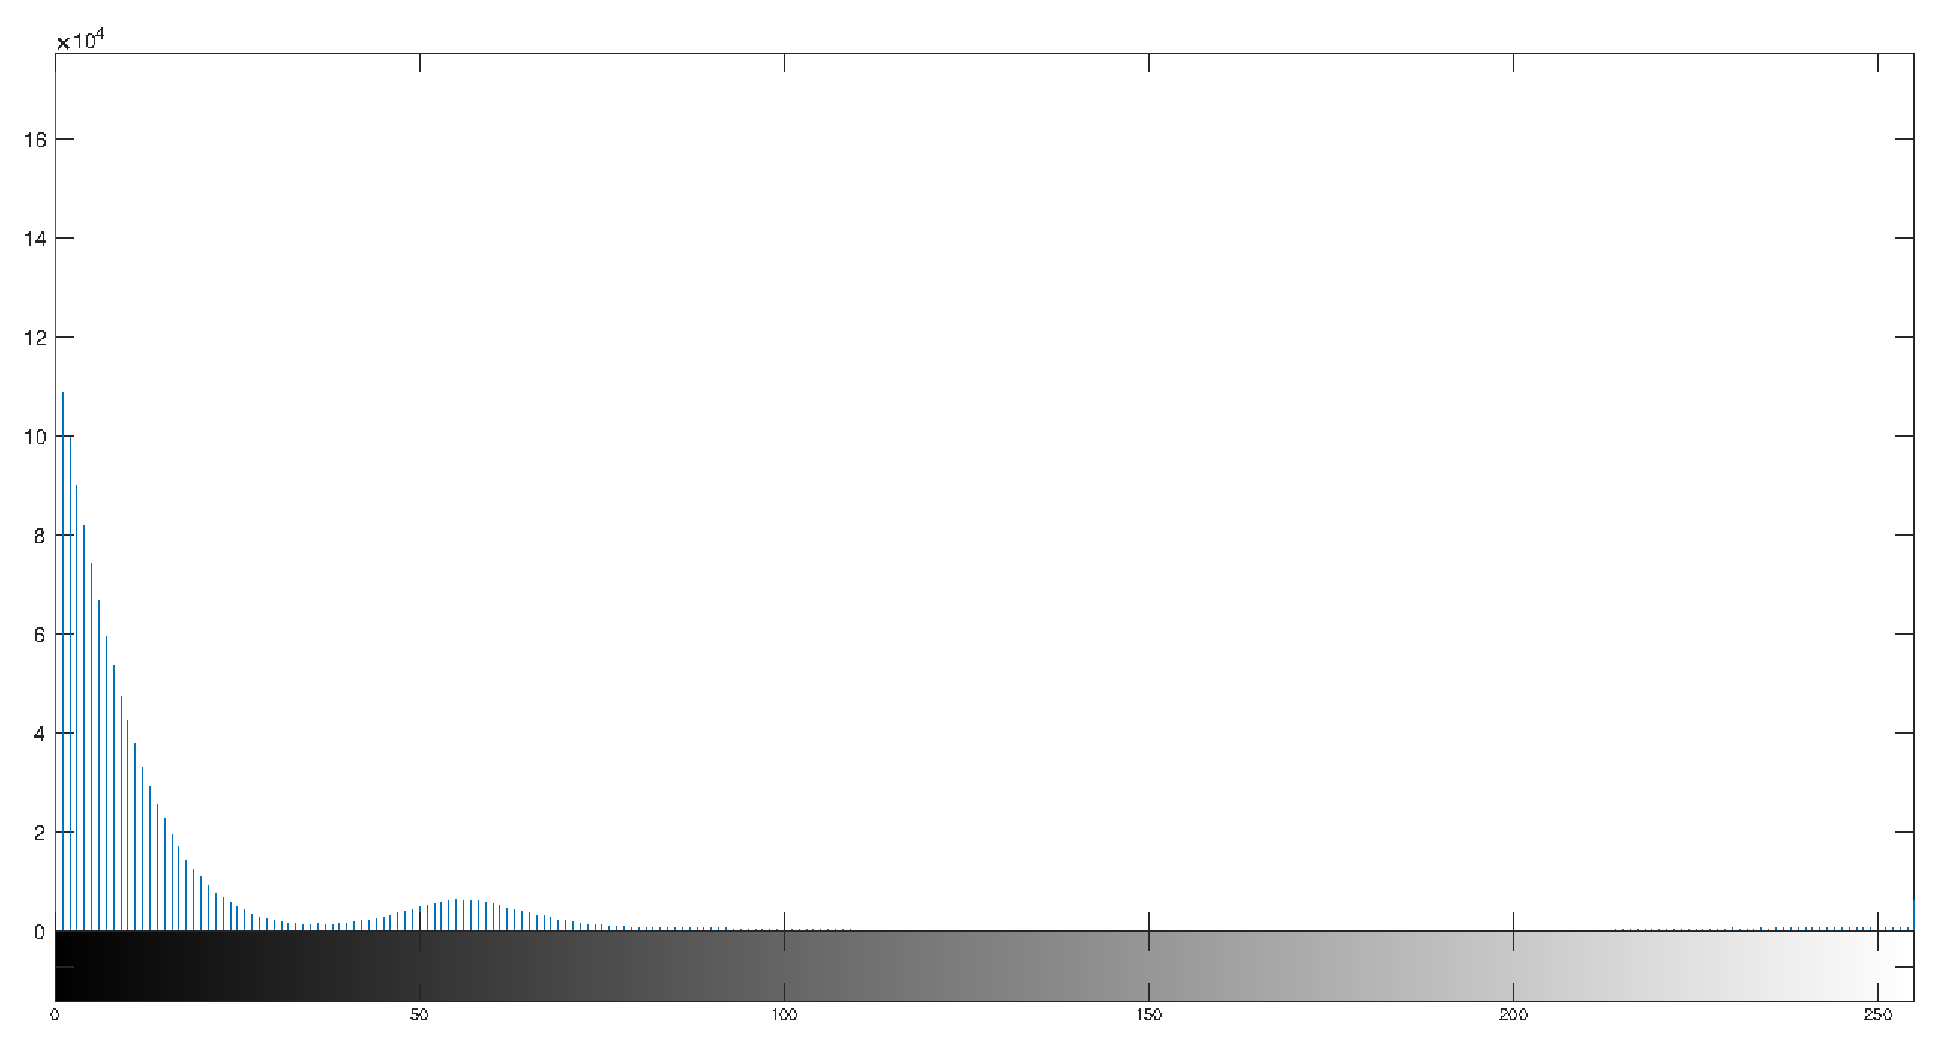
\includegraphics[width=0.45\textwidth]{gfx/comparison/comp1/4.eps}}
  \qquad
  \subfloat[Sobel image.]{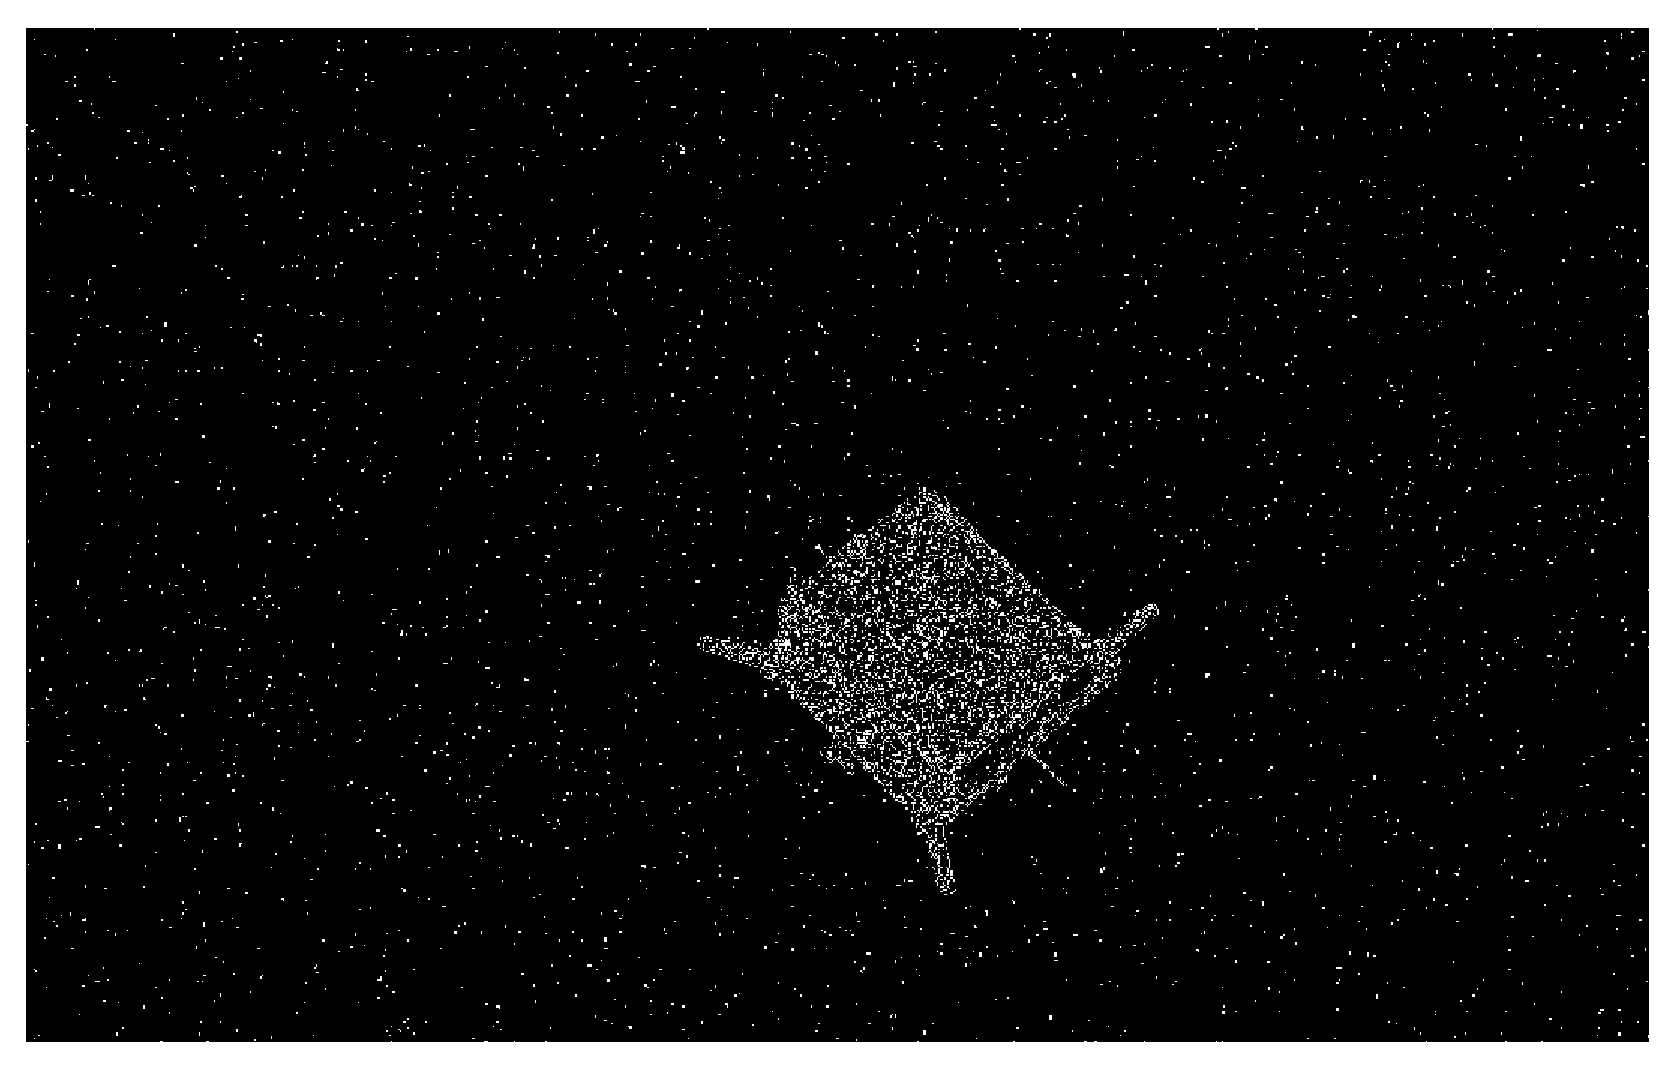
\includegraphics[width=0.45\textwidth]{gfx/comparison/comp1/5.eps}}
  \qquad
  \subfloat[Sobel image.]{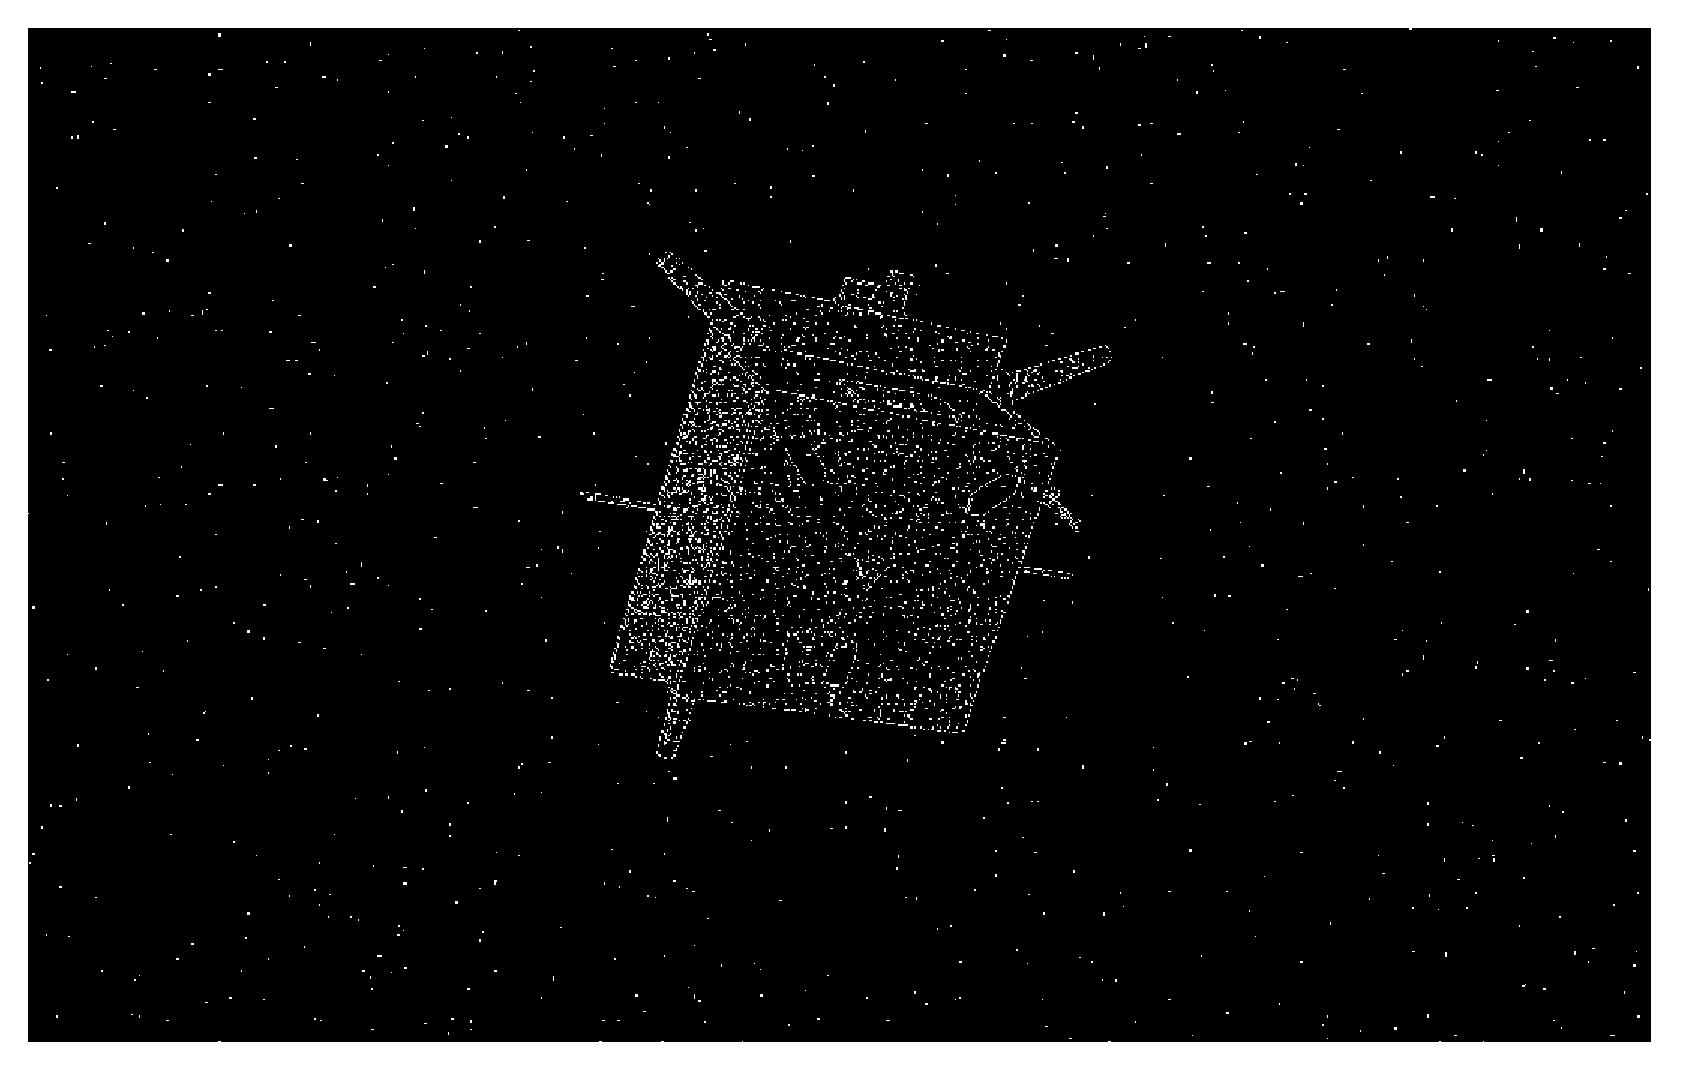
\includegraphics[width=0.45\textwidth]{gfx/comparison/comp1/6.eps}}
  \qquad
  \caption{Comparison between the SPEED data-set (left) and images generated using the toolbox presented in Chapter~\ref{chap:second-chapter} (right), (1).}
  \label{fig:comparison1}
\end{figure}

\begin{figure}[htbp]
  \centering
  \subfloat[Unfiltered image.]{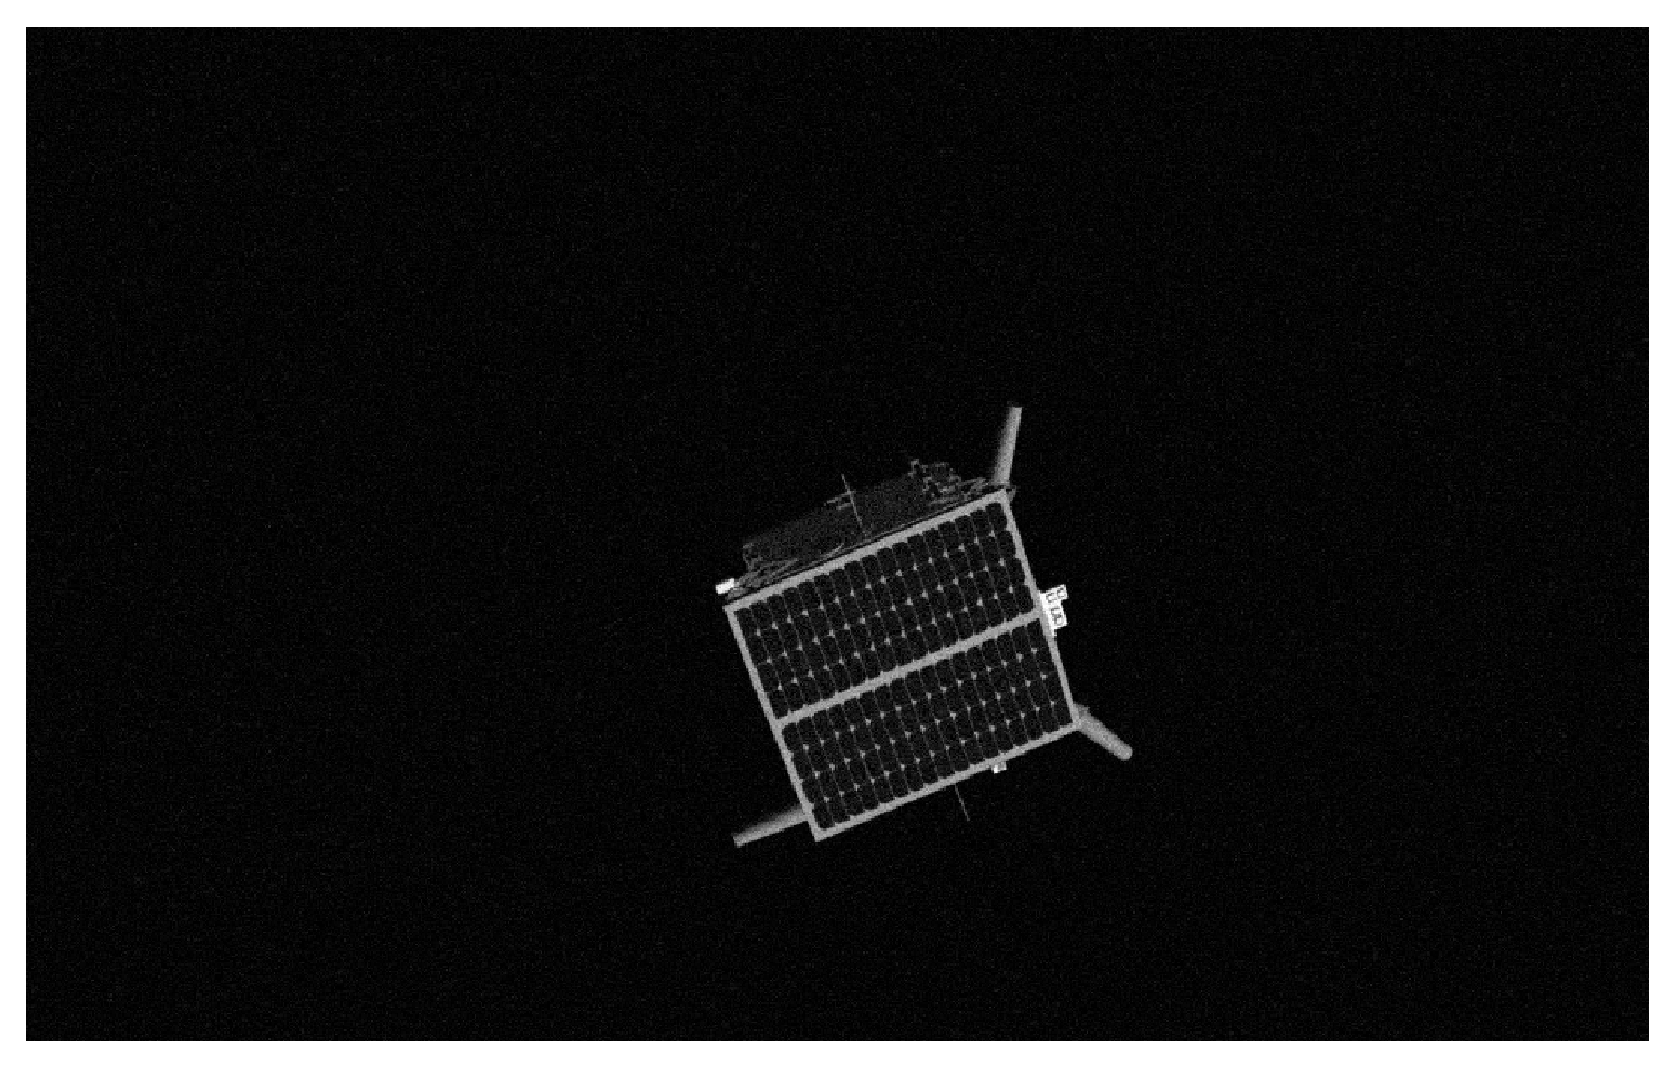
\includegraphics[width=0.45\textwidth]{gfx/comparison/comp2/1.eps}}
  \qquad
  \subfloat[Unfiltered image.]{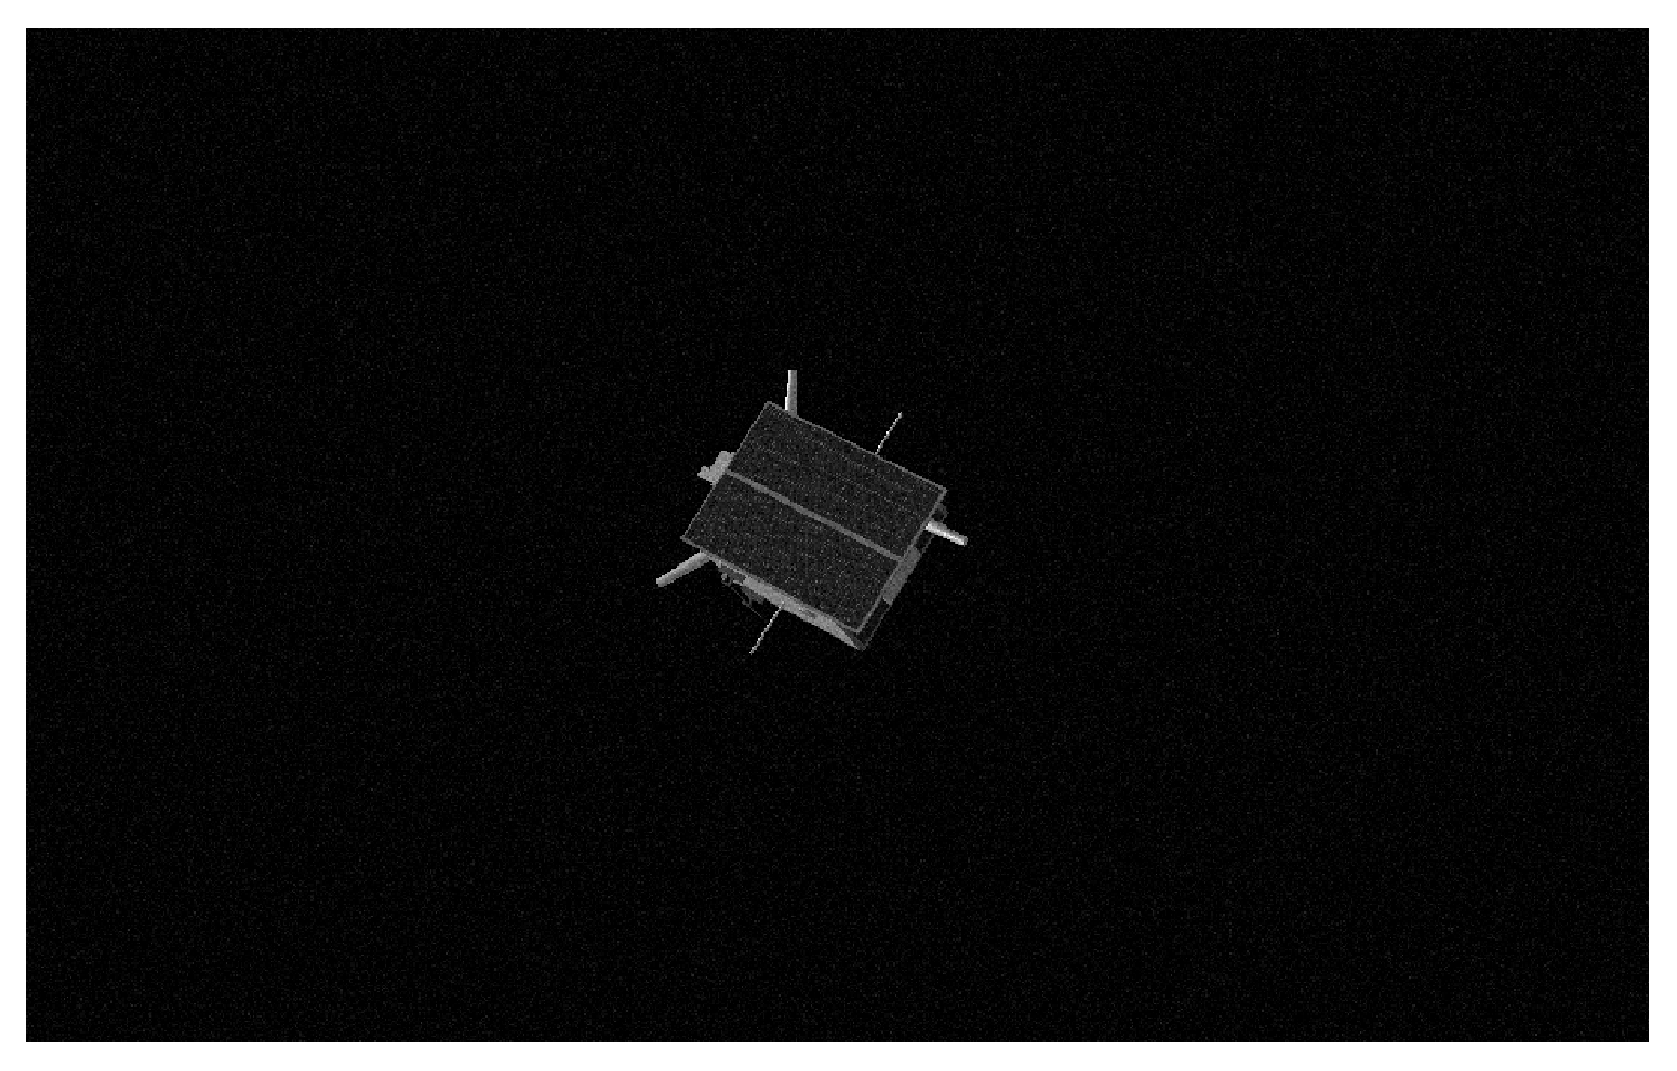
\includegraphics[width=0.45\textwidth]{gfx/comparison/comp2/2.eps}}
  \qquad
  \subfloat[Histogram.]{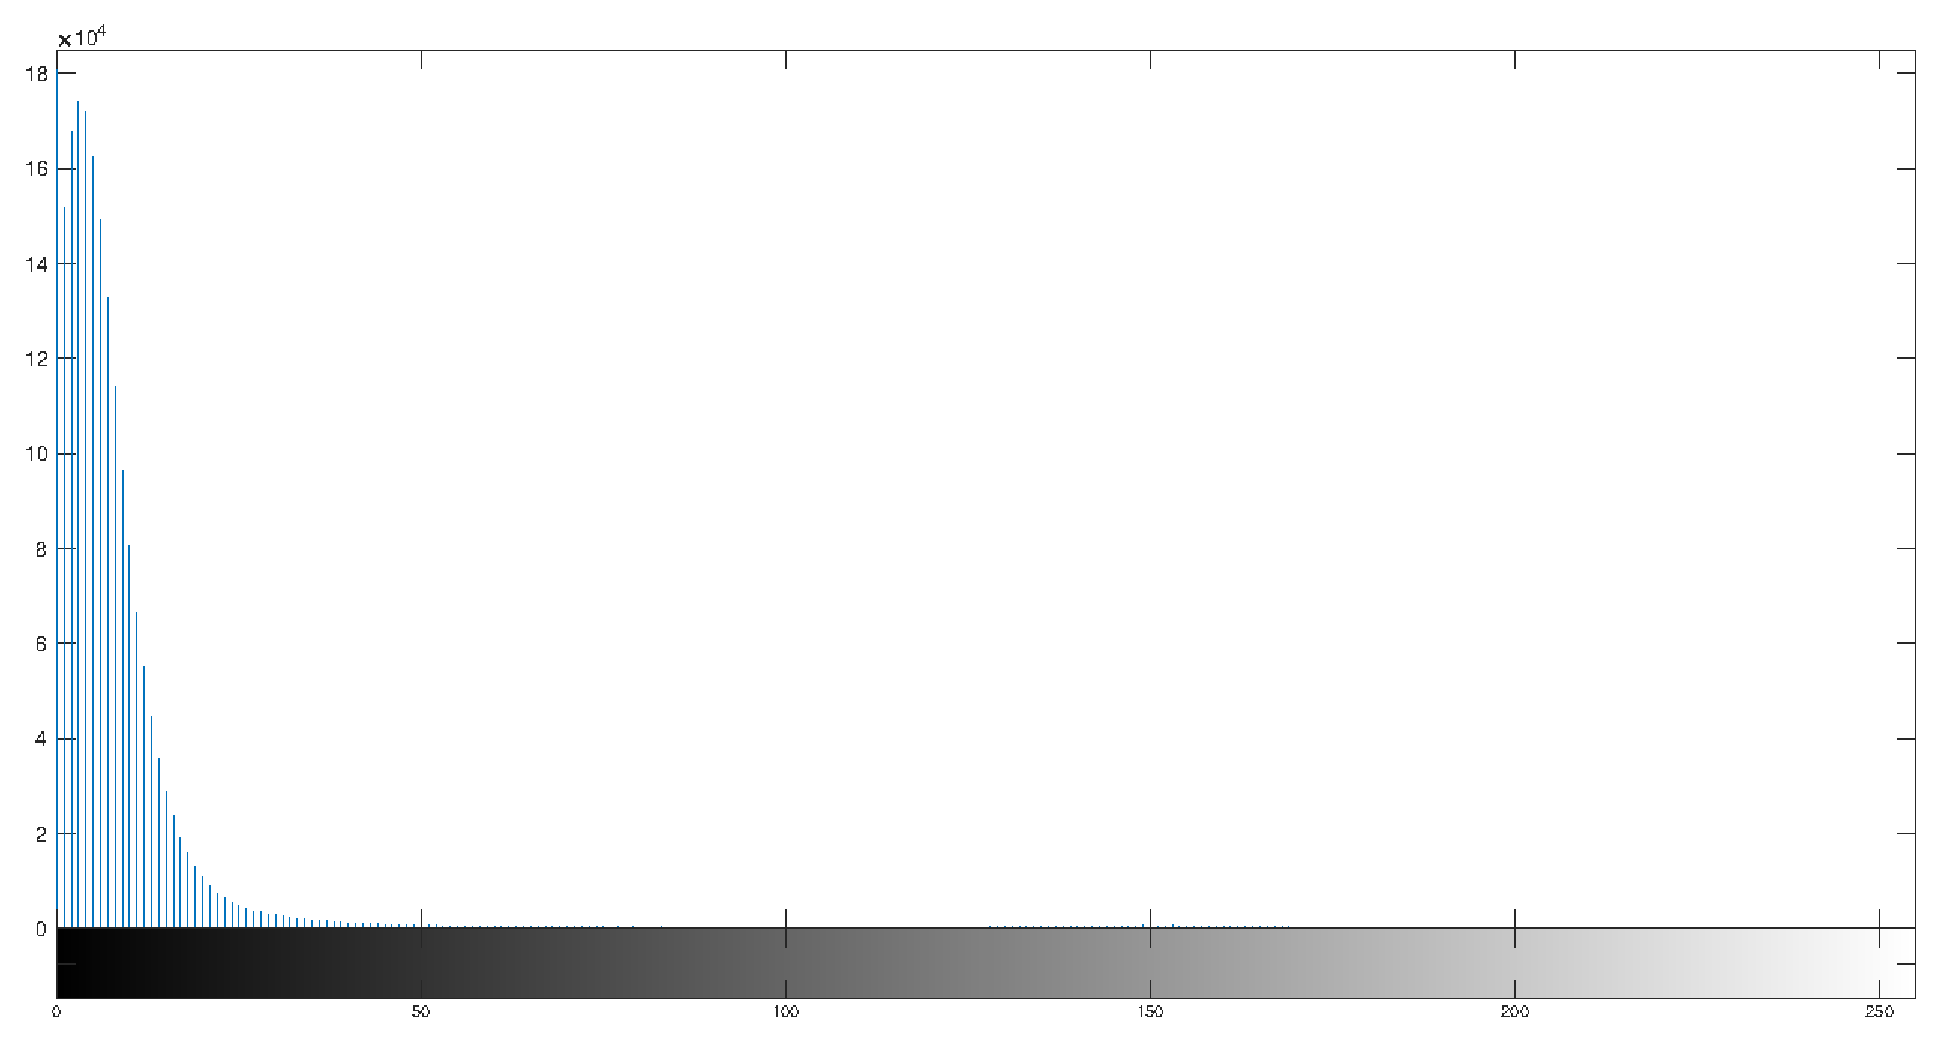
\includegraphics[width=0.45\textwidth]{gfx/comparison/comp2/3.eps}}
  \qquad
  \subfloat[Histogram.]{\includegraphics[width=0.45\textwidth]{gfx/comparison/comp2/4.eps}}
  \qquad
  \subfloat[Sobel image.]{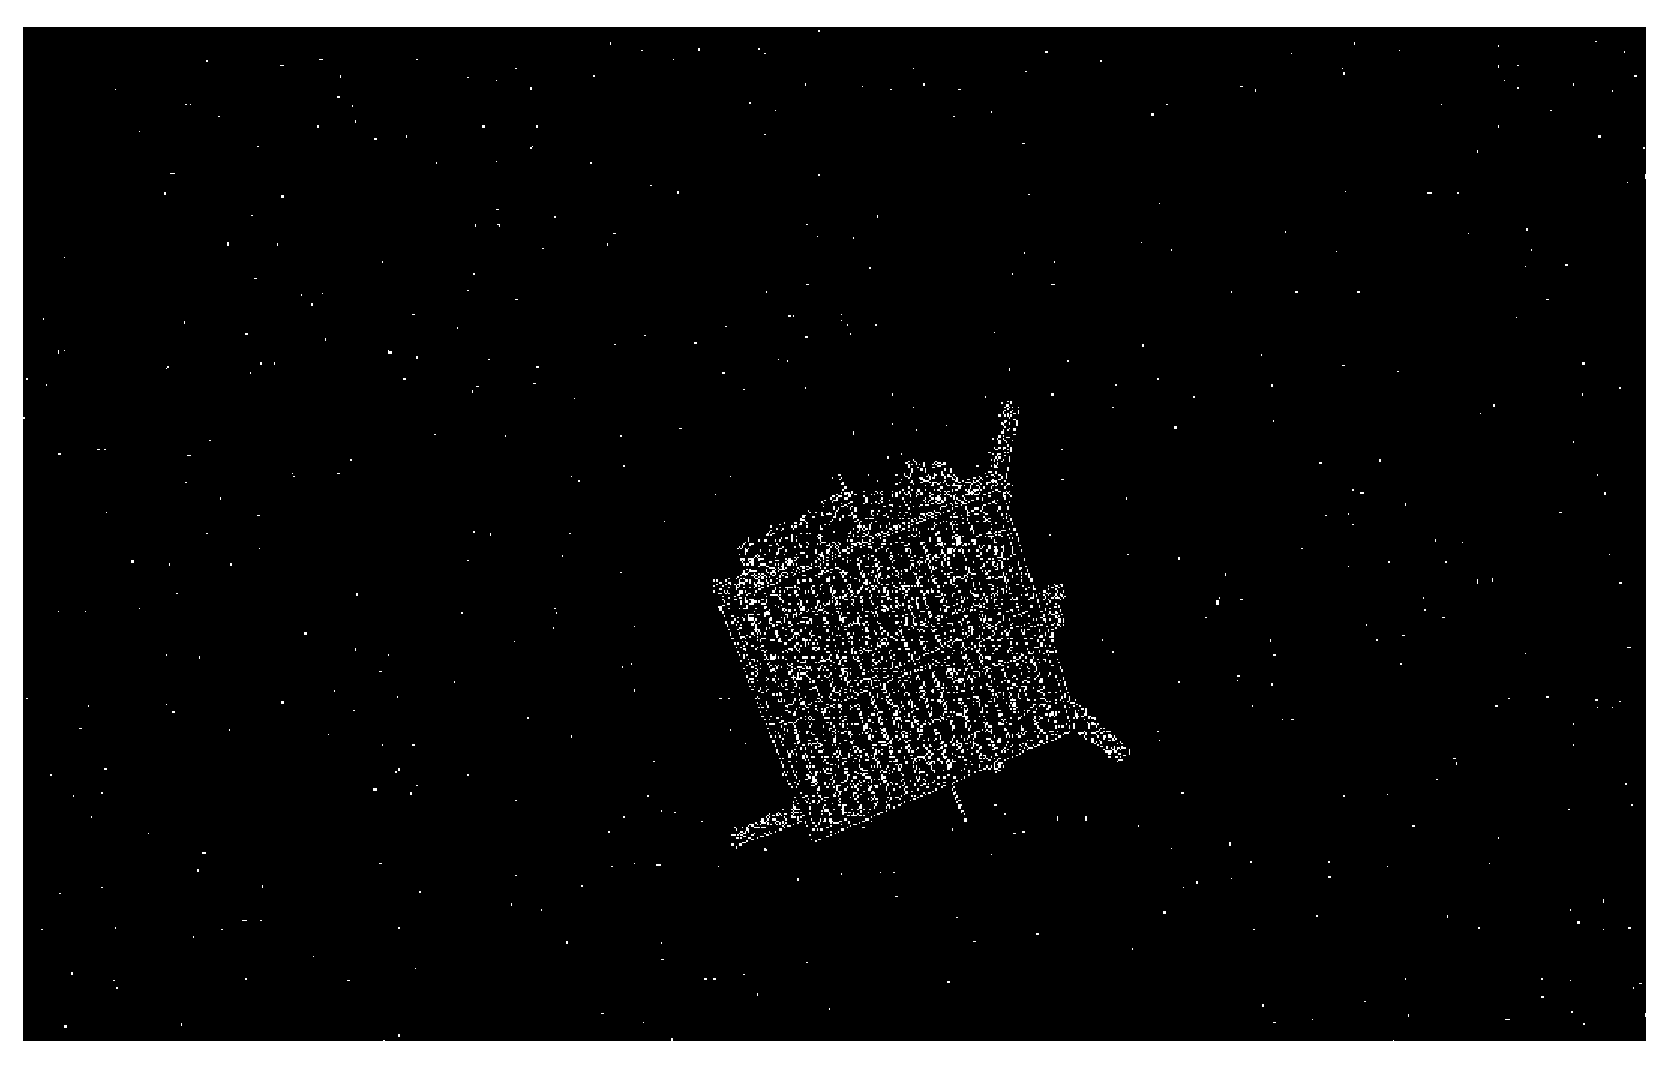
\includegraphics[width=0.45\textwidth]{gfx/comparison/comp2/5.eps}}
  \qquad
  \subfloat[Sobel image.]{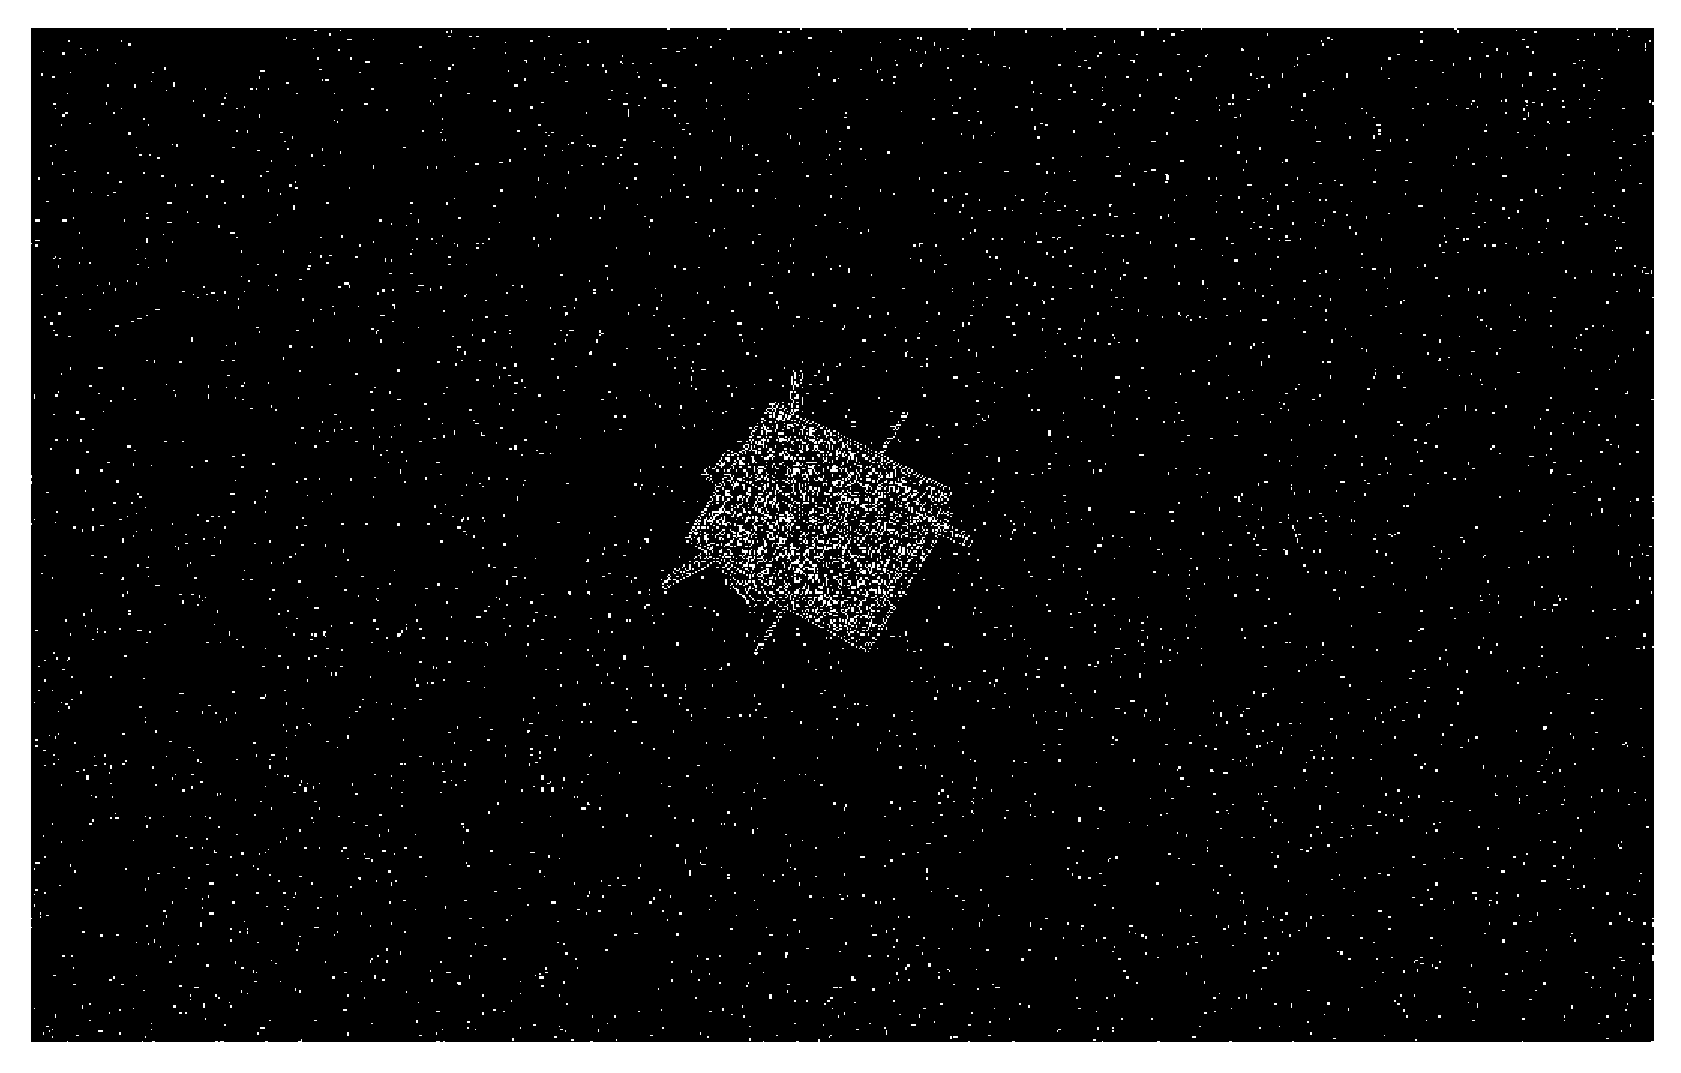
\includegraphics[width=0.45\textwidth]{gfx/comparison/comp2/6.eps}}
  \qquad
  \caption{Comparison between the SPEED data-set (left) and images generated using the toolbox presented in Chapter~\ref{chap:second-chapter} (right), (2).}
  \label{fig:comparison2}
\end{figure}

\begin{figure}[htbp]
  \centering
  \subfloat[Unfiltered image.]{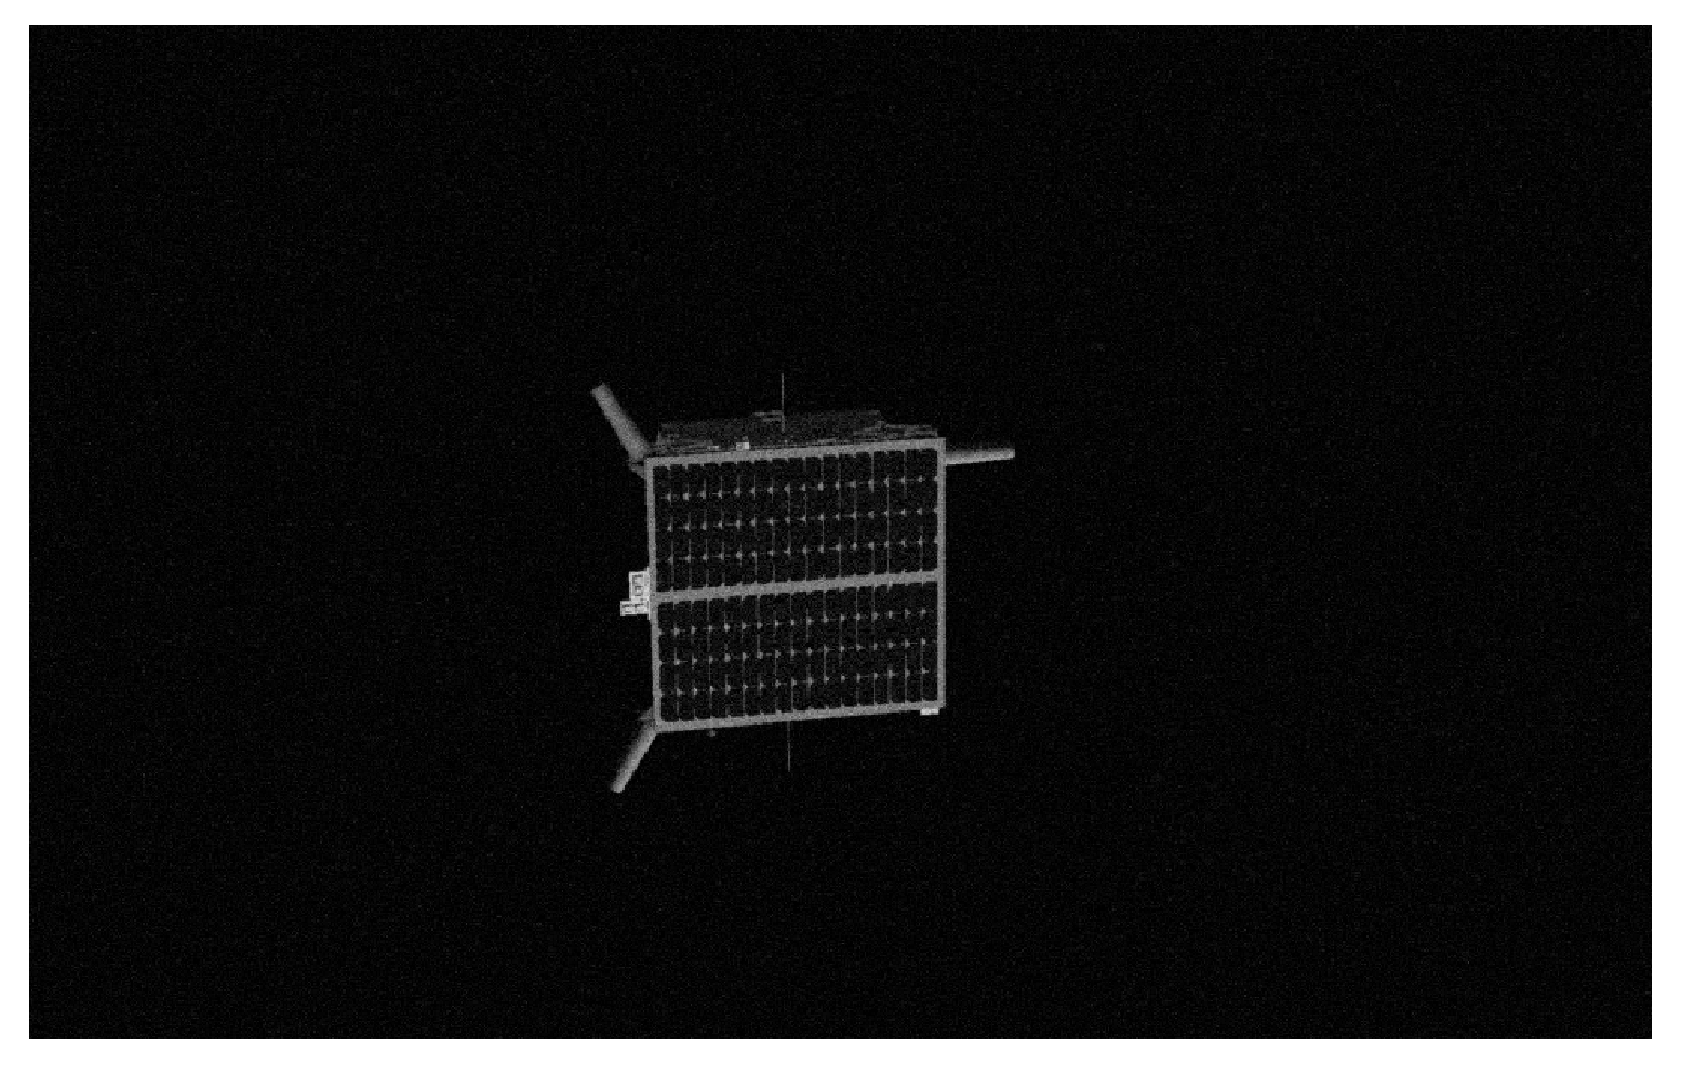
\includegraphics[width=0.45\textwidth]{gfx/comparison/comp3/1.eps}}
  \qquad
  \subfloat[Unfiltered image.]{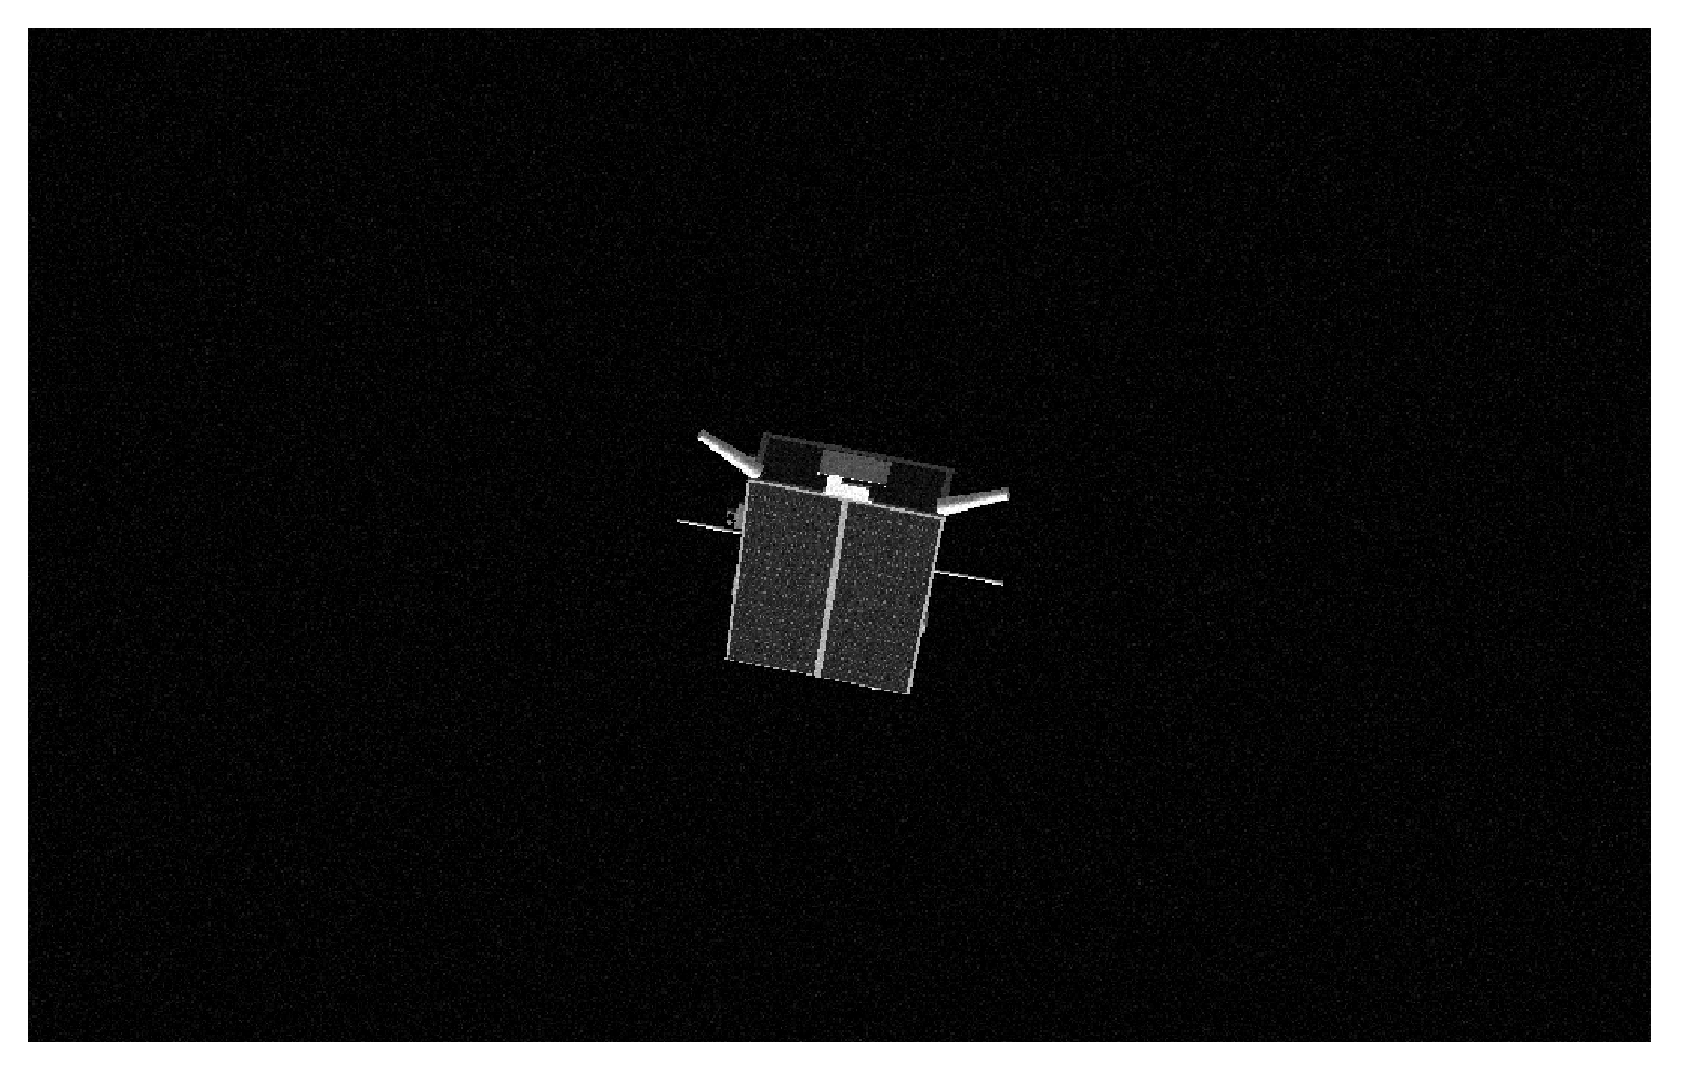
\includegraphics[width=0.45\textwidth]{gfx/comparison/comp3/2.eps}}
  \qquad
  \subfloat[Histogram.]{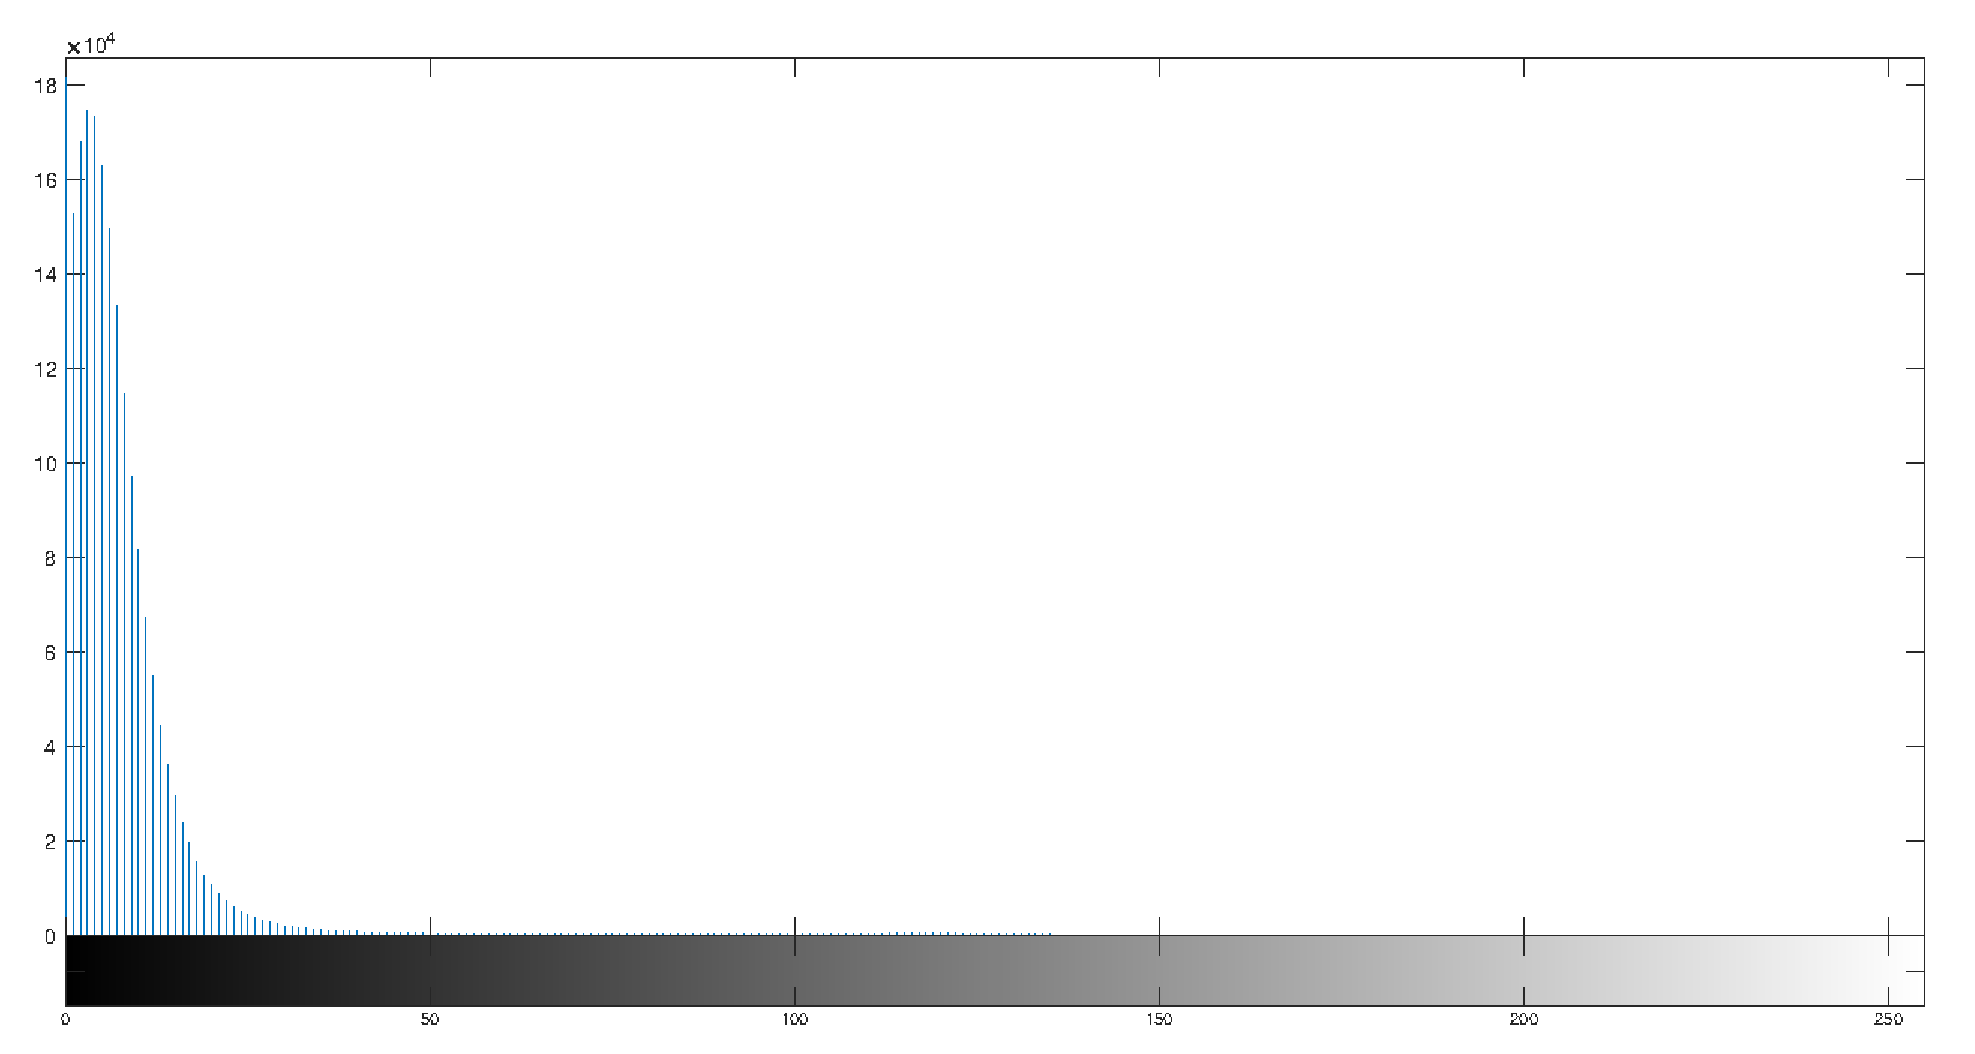
\includegraphics[width=0.45\textwidth]{gfx/comparison/comp3/3.eps}}
  \qquad
  \subfloat[Histogram.]{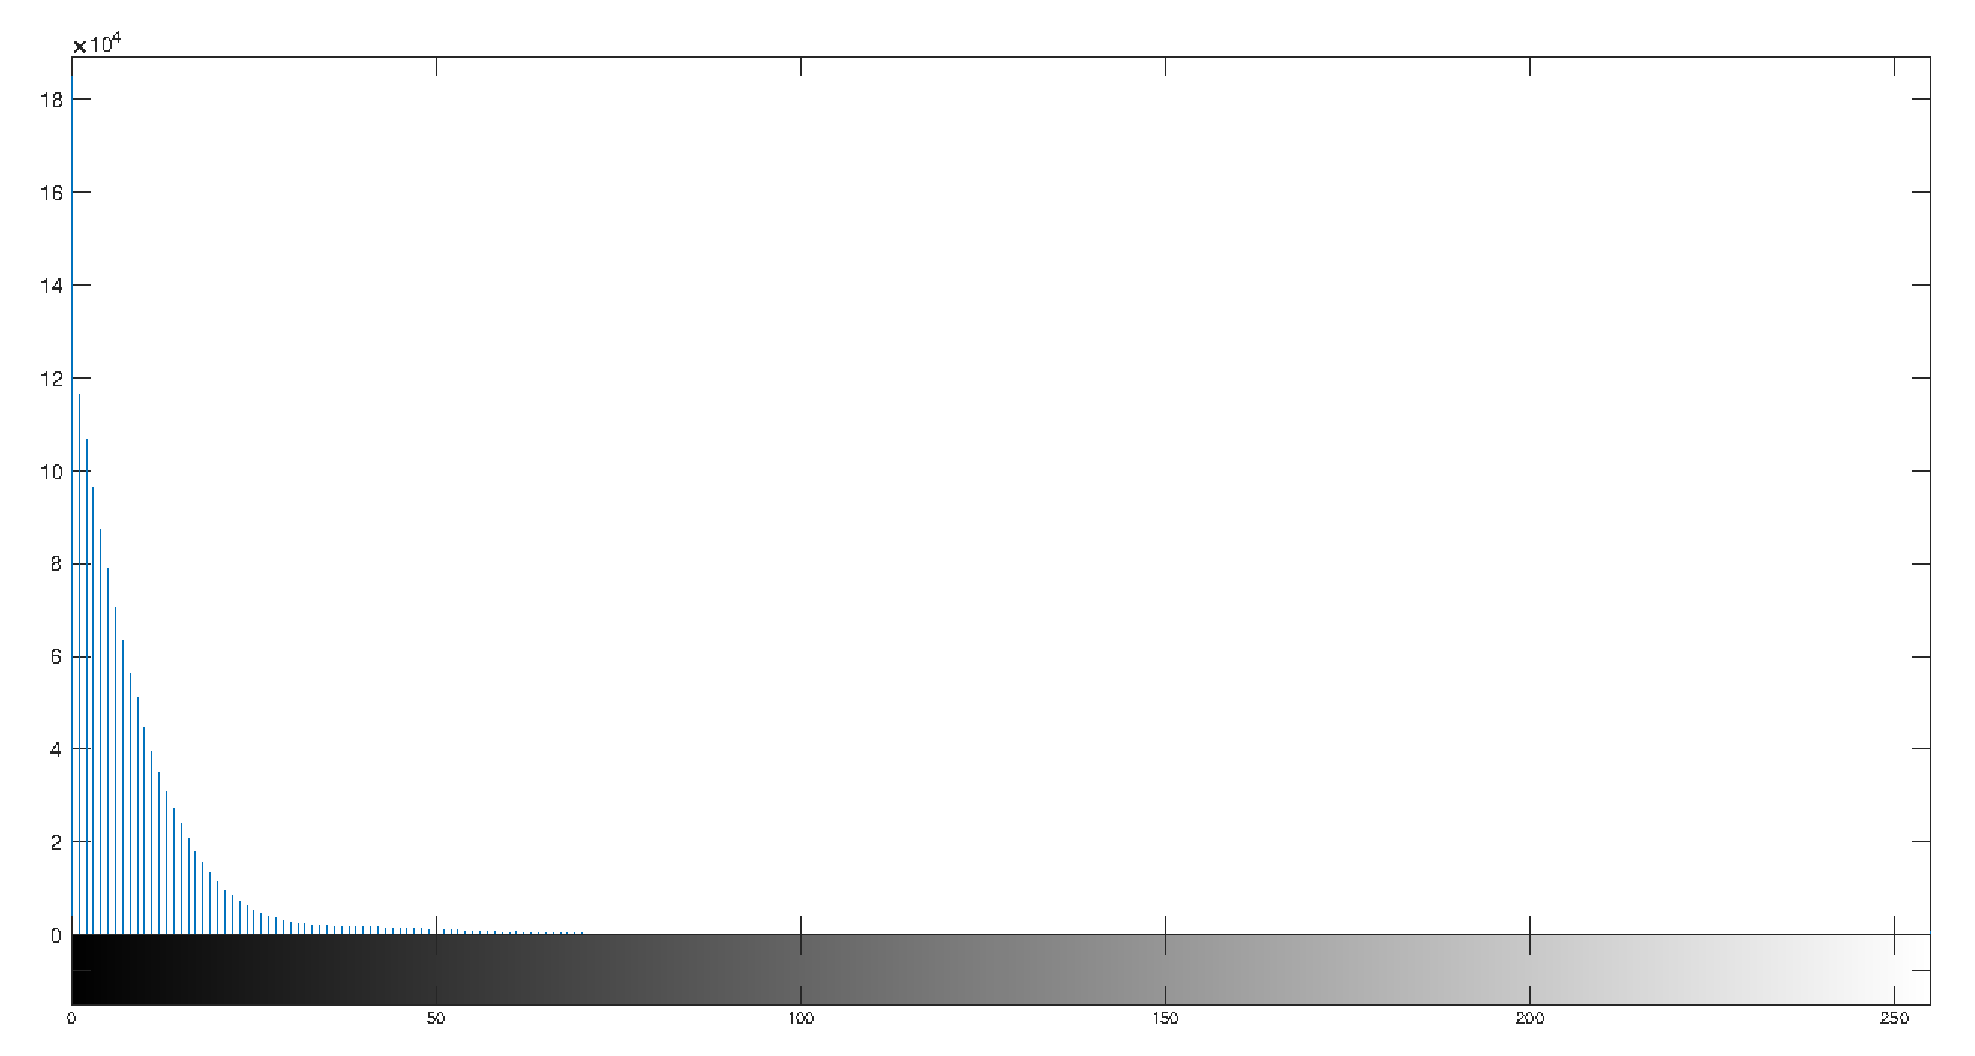
\includegraphics[width=0.45\textwidth]{gfx/comparison/comp3/4.eps}}
  \qquad
  \subfloat[Sobel image.]{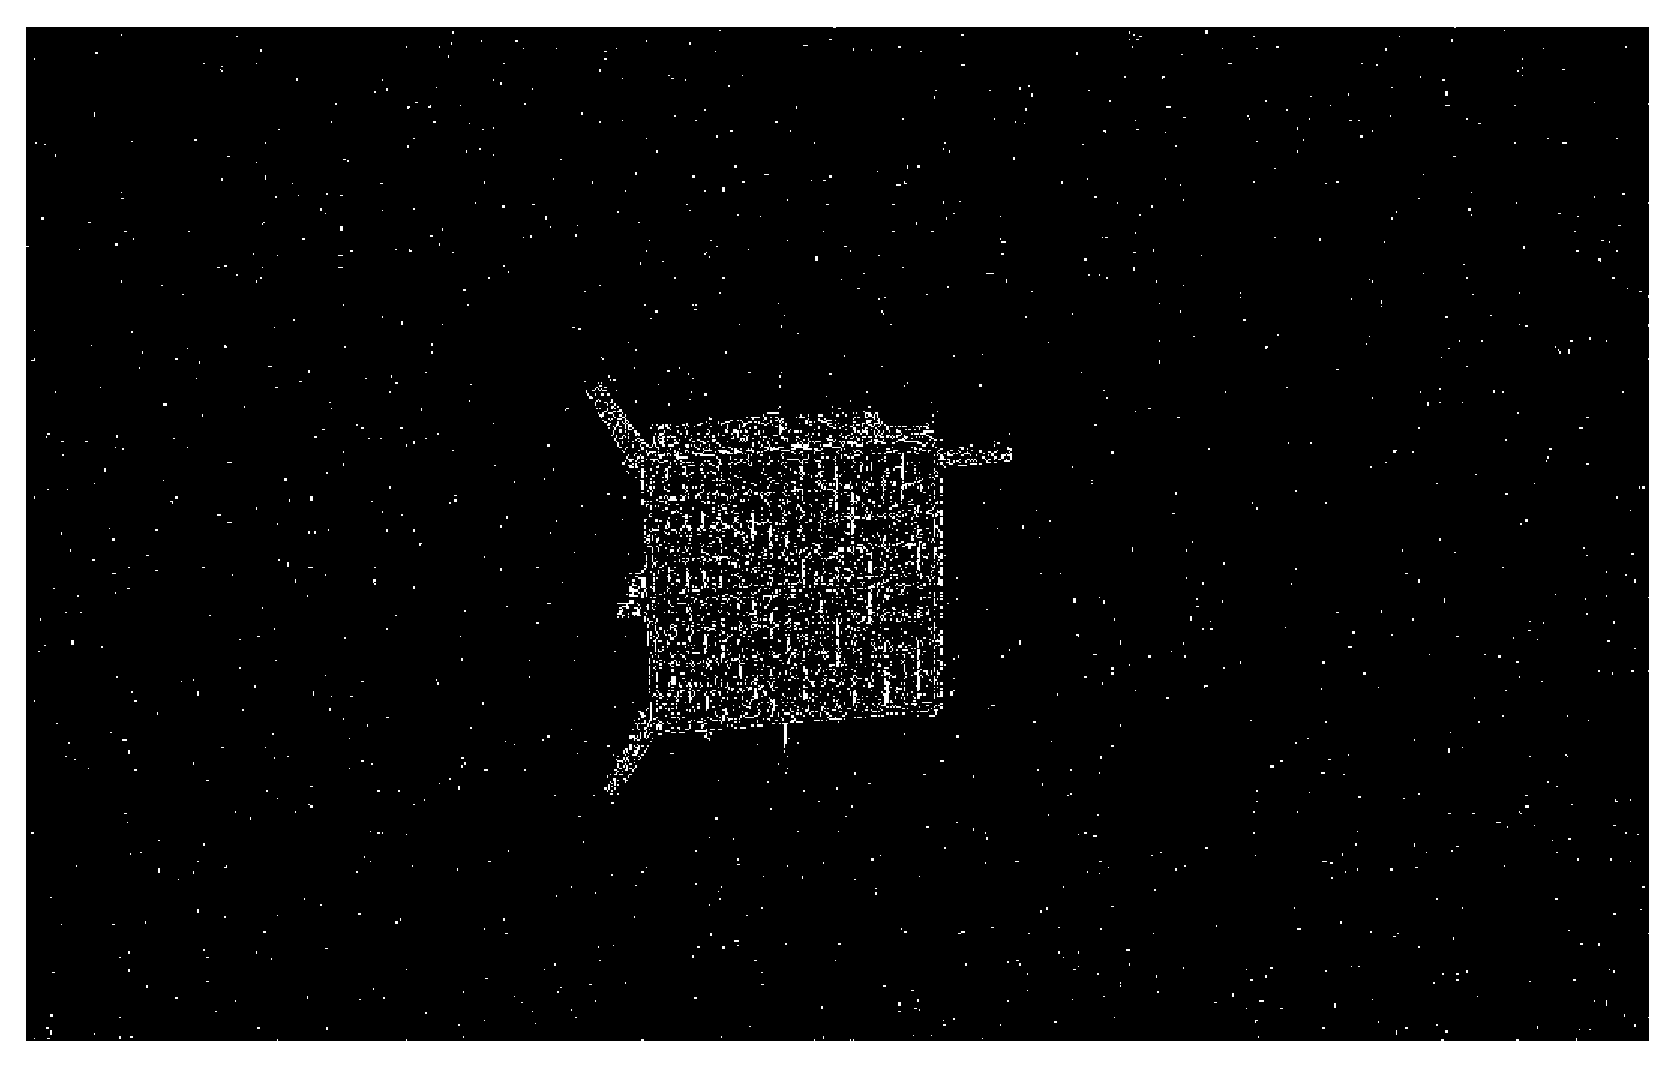
\includegraphics[width=0.45\textwidth]{gfx/comparison/comp3/5.eps}}
  \qquad
  \subfloat[Sobel image.]{\includegraphics[width=0.45\textwidth]{gfx/comparison/comp3/6.eps}}
  \qquad
  \caption{Comparison between the SPEED data-set (left) and images generated using the toolbox presented in Chapter~\ref{chap:second-chapter} (right), (3).}
  \label{fig:comparison3}
\end{figure}

\begin{figure}[htbp]
  \centering
  \subfloat[Unfiltered image.]{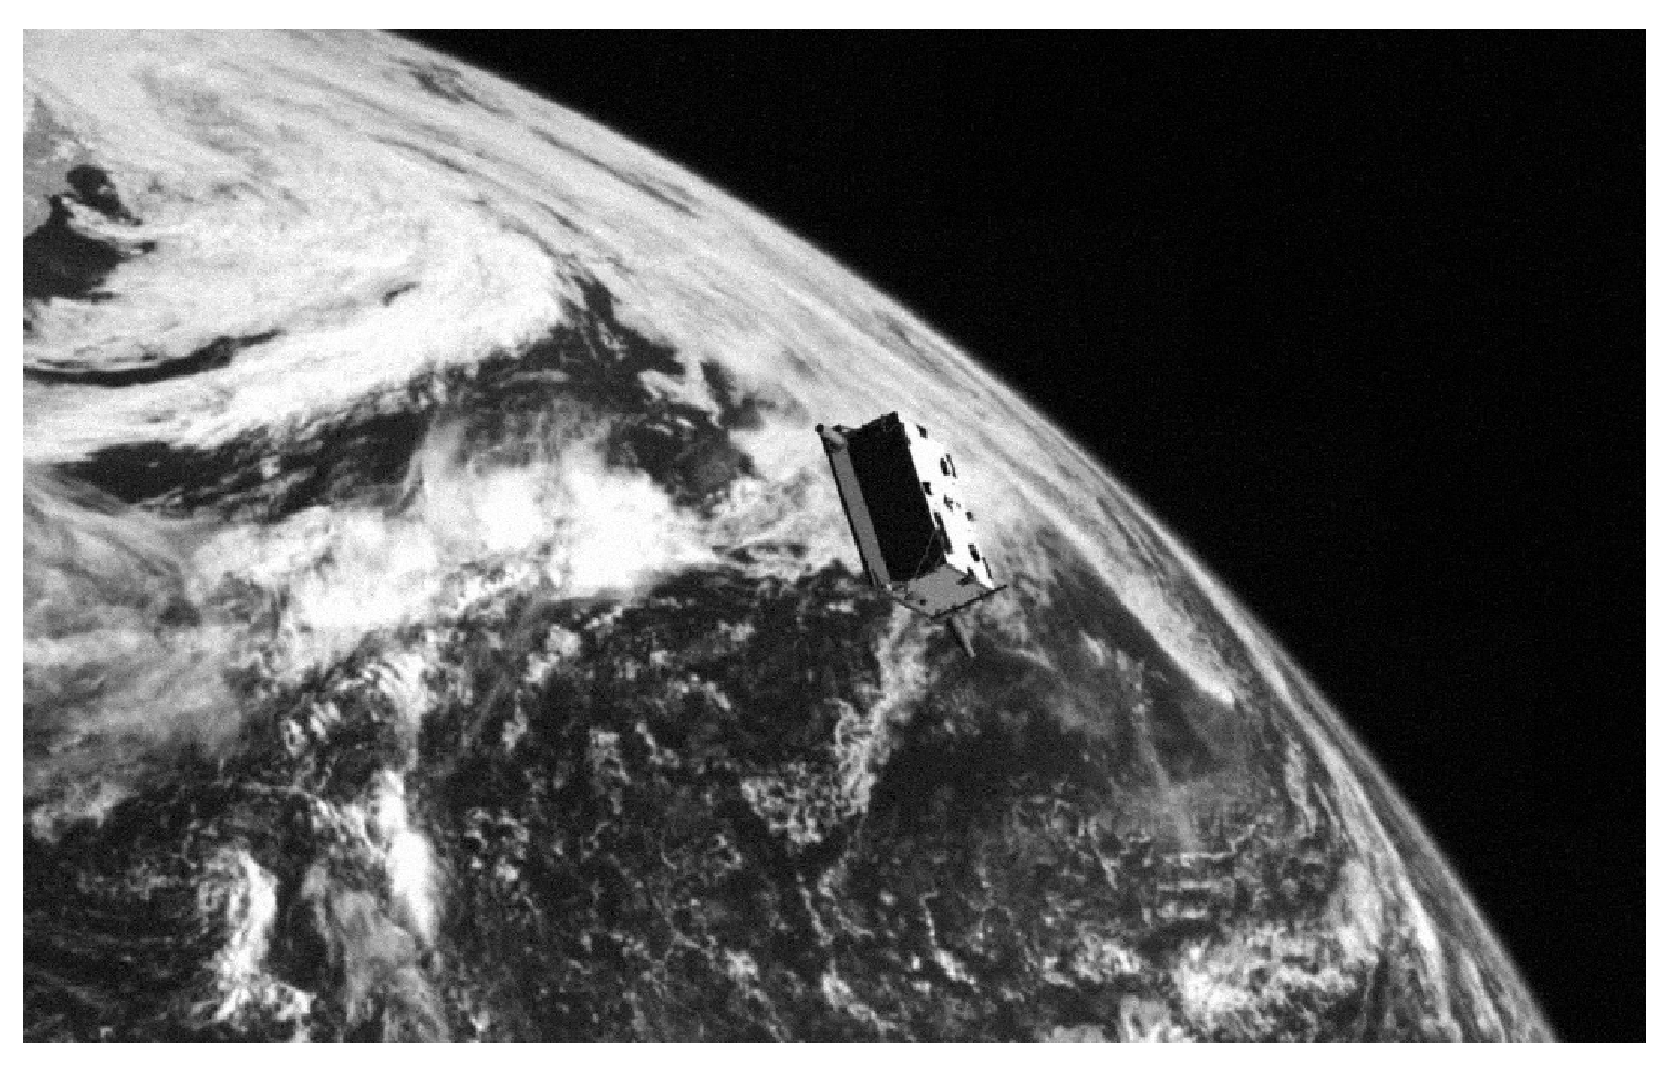
\includegraphics[width=0.45\textwidth]{gfx/comparison/comp4/1.eps}}
  \qquad
  \subfloat[Unfiltered image.]{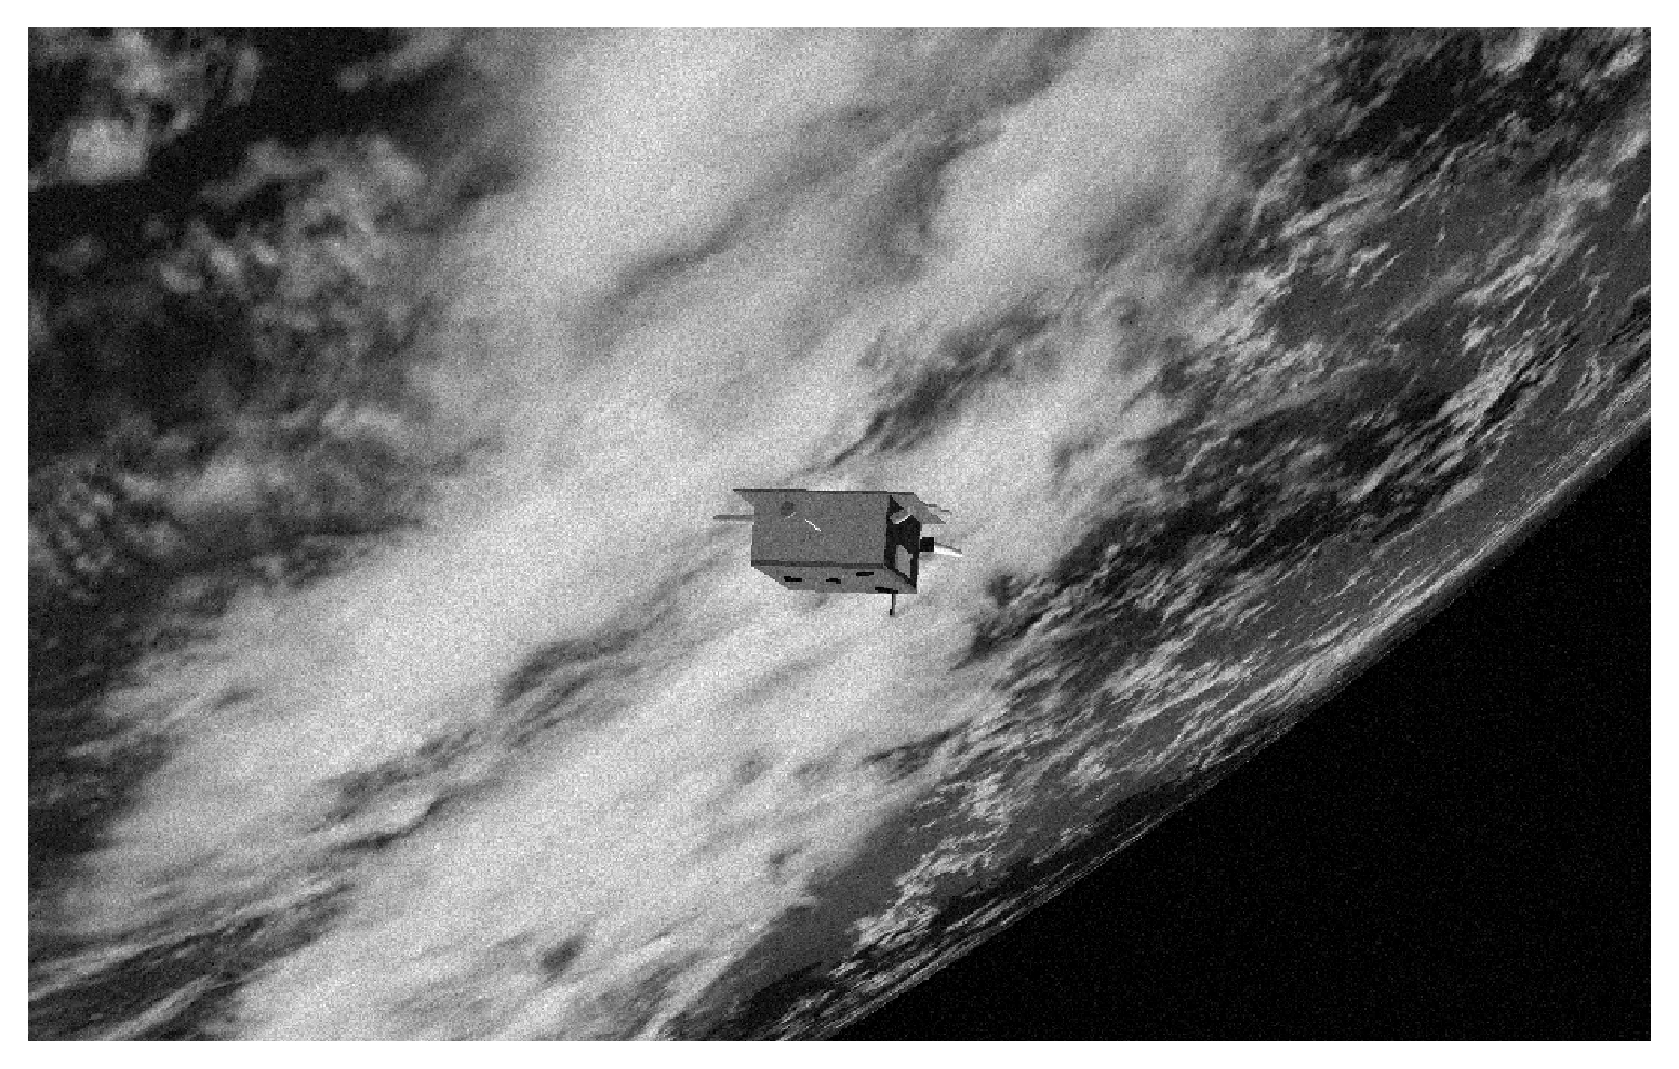
\includegraphics[width=0.45\textwidth]{gfx/comparison/comp4/2.eps}}
  \qquad
  \subfloat[Histogram.]{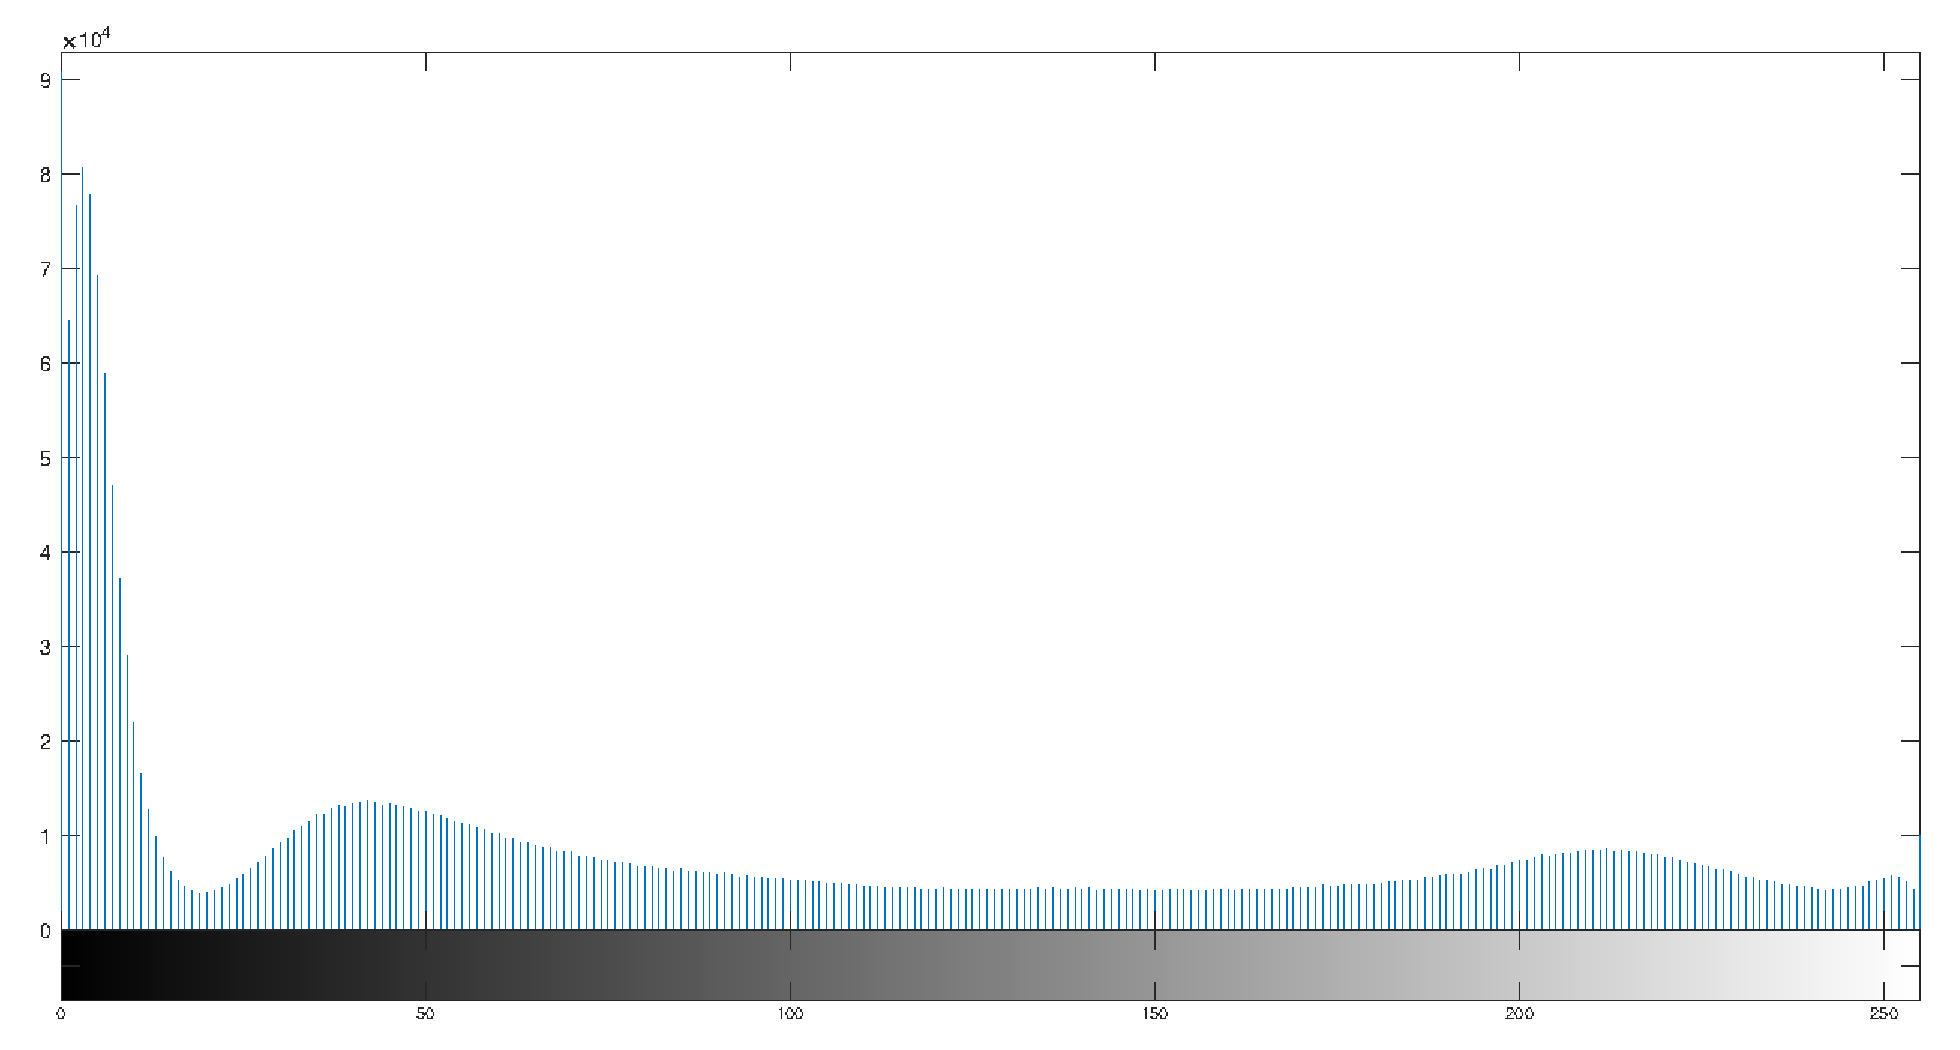
\includegraphics[width=0.45\textwidth]{gfx/comparison/comp4/3.eps}}
  \qquad
  \subfloat[Histogram.]{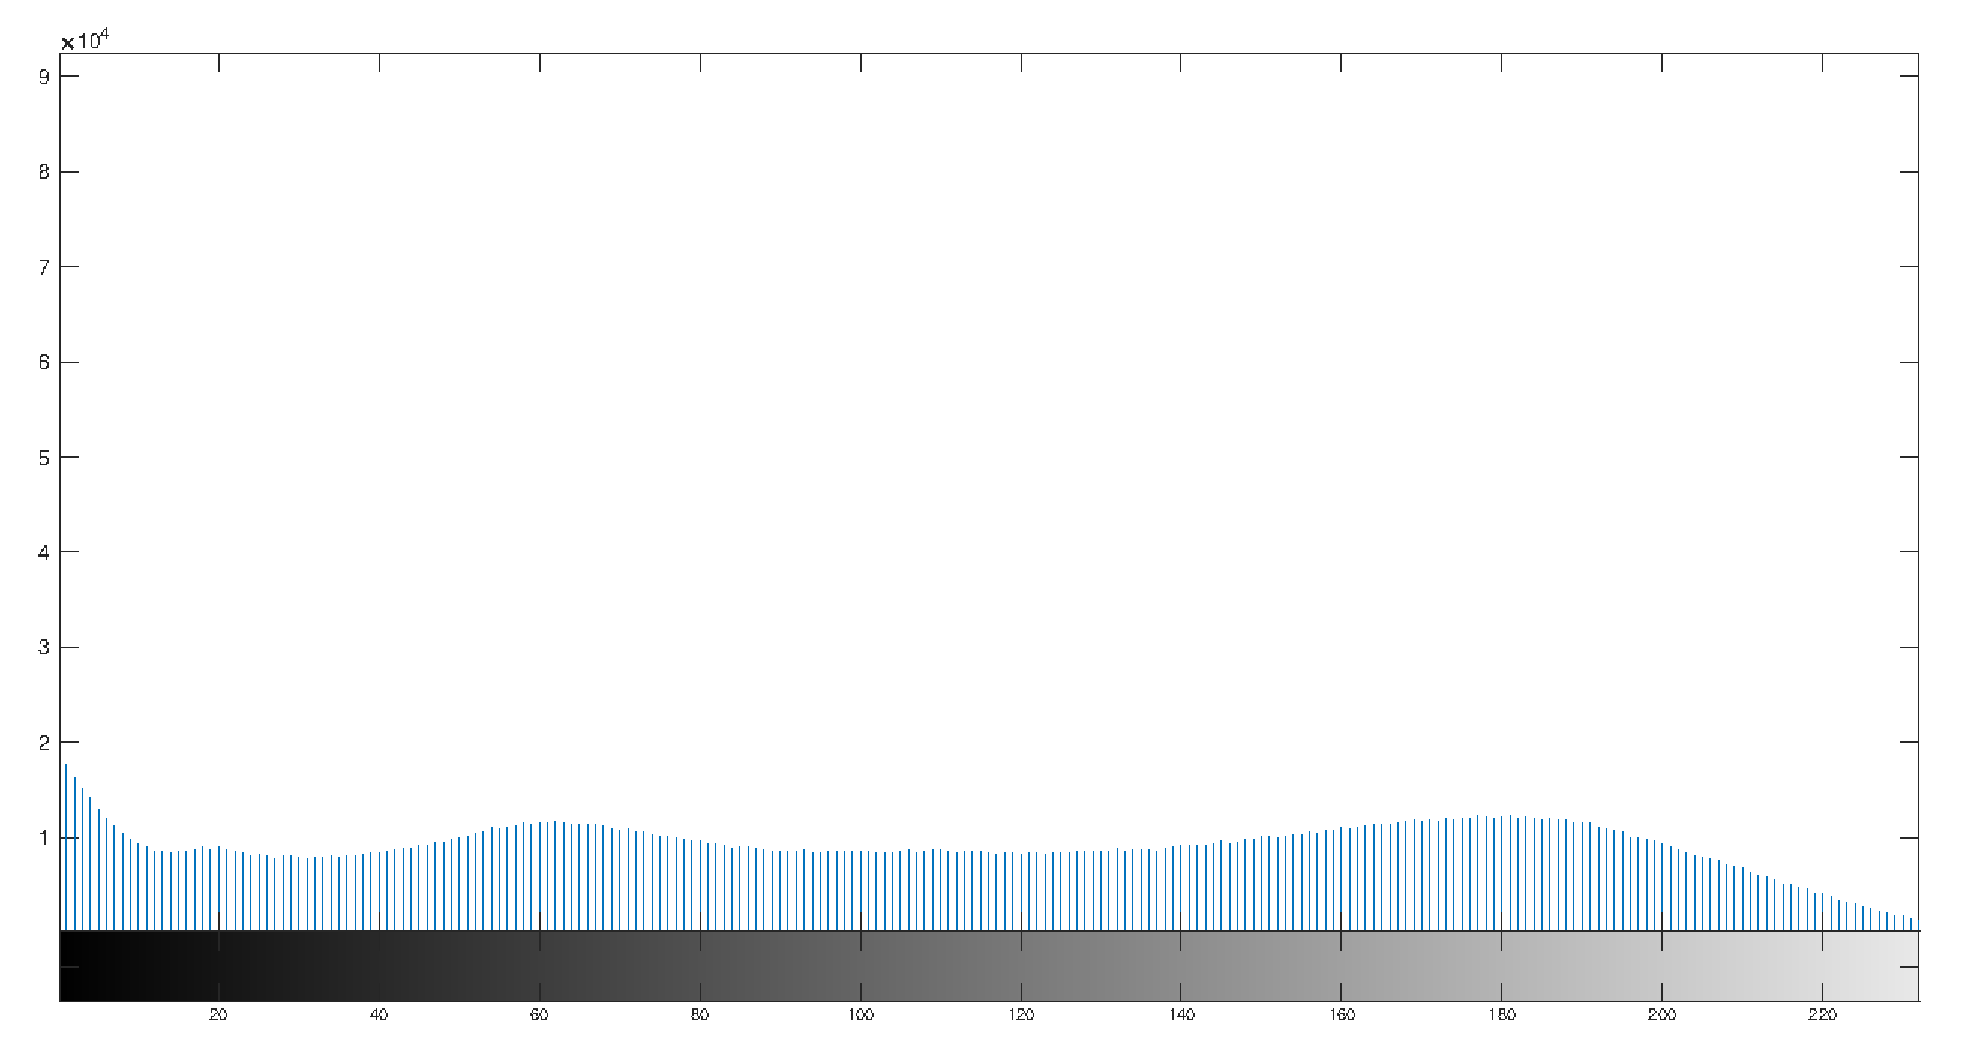
\includegraphics[width=0.45\textwidth]{gfx/comparison/comp4/4.eps}}
  \qquad
  \subfloat[Sobel image.]{\includegraphics[width=0.45\textwidth]{gfx/comparison/comp4/5.eps}}
  \qquad
  \subfloat[Sobel image.]{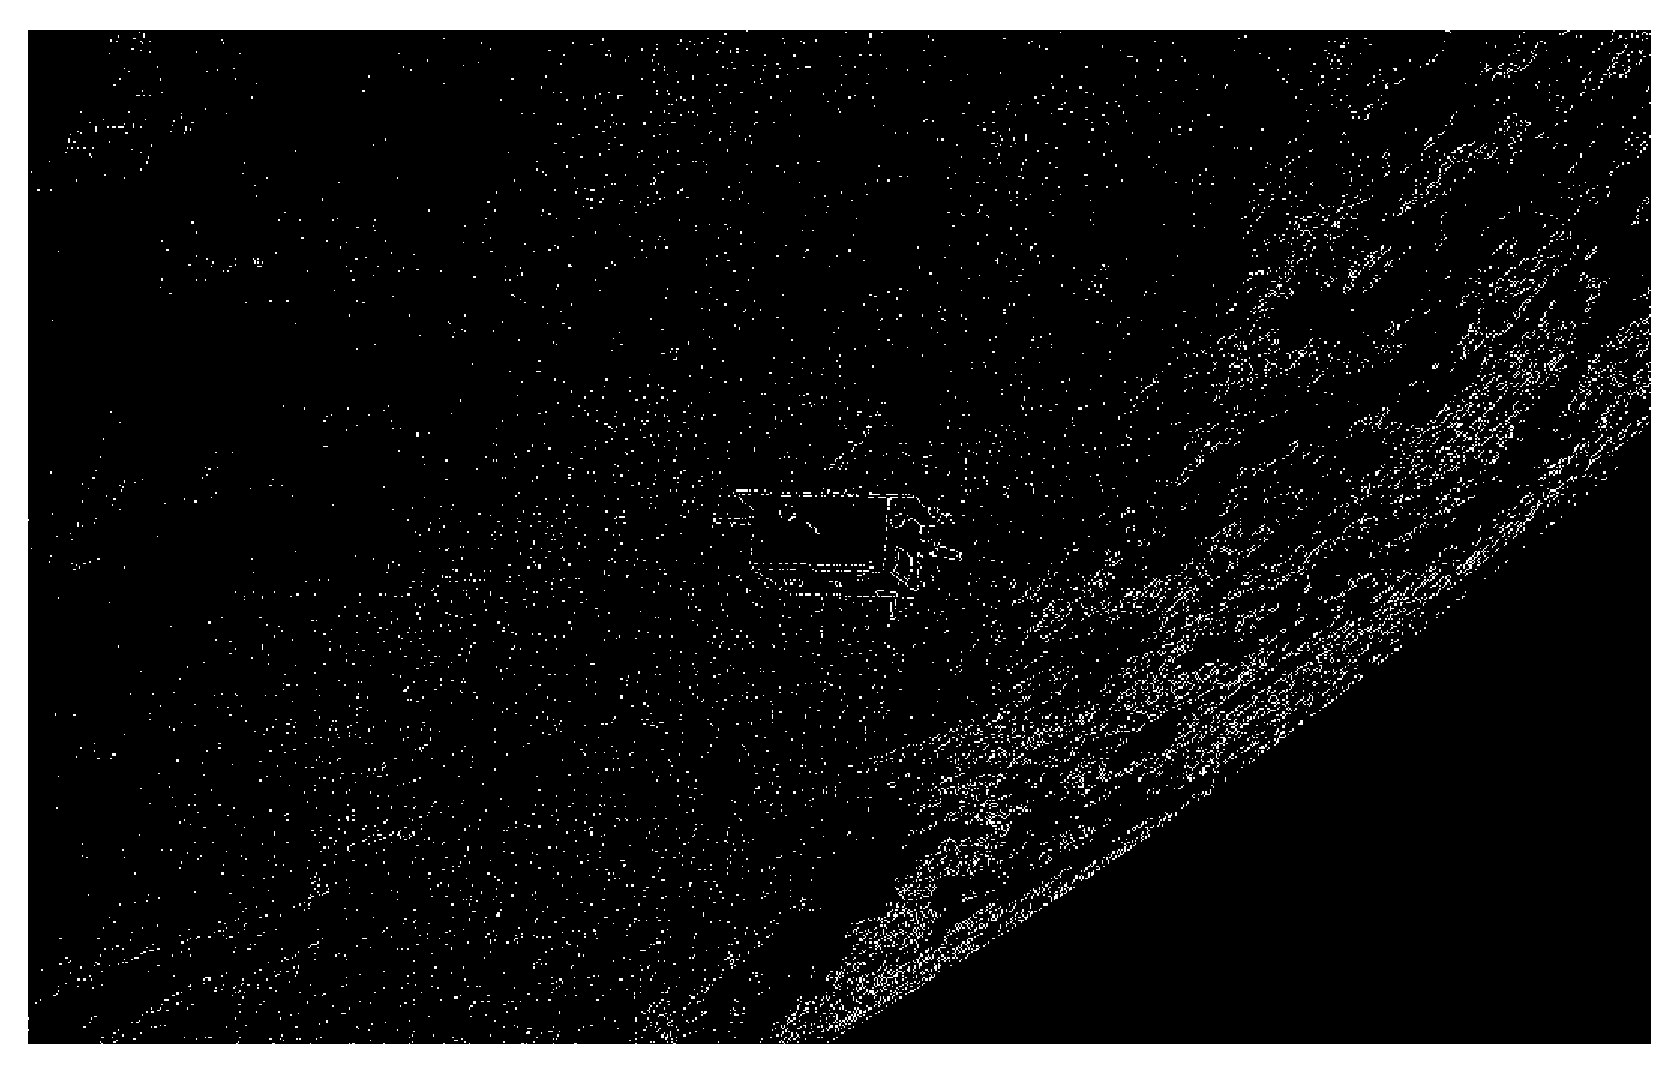
\includegraphics[width=0.45\textwidth]{gfx/comparison/comp4/6.eps}}
  \qquad
  \caption{Comparison between the SPEED data-set (left) and images generated using the toolbox presented in Chapter~\ref{chap:second-chapter} (right), (4).}
  \label{fig:comparison4}
\end{figure}

In Figures~\ref{fig:comparison1}, \ref{fig:comparison2}, \ref{fig:comparison3} are presented three simulated images of the Tango \acrshort{sc} on a black background.
Overall, it is possible to recognize that the images belonging to the SPEED shows a better representation of the external look of the \acrshort{sc}, for both the solar panels, the external appendages and the external structures. This is not an issue of the technique used to render the images by itself, but merely depends from the availability of adequate textures to render the \acrshort{sc}. Usually, the manufacturer makes available textures of the external look of the whole \acrshort{sc}. For this project unfortunately, due to the unavailability of said textures, the whole look of had to be recreated by hand, doing several experiments and comparisons. This is particularly visible when looking at solar panels, where the SPEED images are of an order of magnitude superior in terms of accuracy and realness of what is being represented.
Despite said issues however, by looking at the forms of the histograms it is possible to recognize that histograms belonging to the SPEED images and histograms belonging to the images used though this project are essentially similar. They both shows the same exponential behavior. The images belonging to the SPEED data-set shows an overall greater concentration of dark values with respect to the ones generated with the toolbox presented in Chapter~\ref{chap:second-chapter}. This is likely to be due to slightly different scenes being represented in terms of illumination conditions and shadows.
The Sobel edge images are also very similar. The images generated for this project presents a slightly higher level of noise (recognizable by the more presence of little white pixels). This can be due to different $\sigma^2$ value used to add Gaussian white noise to the image during the post-processing phase. As said for the textures, this is not an issue of the technique employed to render the image. Usually the amount of noise to add to the image during the post-processing phase depends on the intrinsic characteristics of the camera which is being simulated. For this work has been decided to mimic as much as possible the behavior of the SPEED data-set, but in general, the amount of noise to add is a parameter which can be tuned to obtain the desired result.
Lastly, in Figure~\ref{fig:comparison4} is showed a comparison were the Earth is in the background. As it can be clearly seen by the reader, the Earth is represented more accurately in the SPEED data-set, but this is simply due to the fact that for the SPEED data-set the Earth images comes from actually real space imagery. As described in \cite{Sharma2019}, the Earth images used for the SPEED data-set are composed by 72 actual images of the Earth captured by the Himawari-8 geostationary meteorological satellite. The 72 images each provide a \num{100e6} pixels resolution disk-view of the Earth and were taken 10 minutes apart from each other over a period of 12 hours. The quality the Earth has in the images generated with the toolbox developed during this work can be enhanced by using a texture with an higher resolution, however this comes at the cost of long rendering times and greater RAM usage for rendering the single image. Generating one single image where the Earth is present in the background takes approximately \SI{3}{\s} and occupy \textit{circa} $2$ Gb of RAM on an Intel Core i7-4500U CPU when using mercator images rescaled to $21600 \times 10800$ pixel resolution. Better results can be achieved using the full $43200 \times 21600$ pixel original mercator images but rendering times as well as RAM usage would grow too much for the generation of a data-set of hundreds of images on the previously mentioned H/W. Obviously, this limit can be overcome by employing a more suitable workstation.

\section{\acrshort{svd} Architecture Tests}
A further validation of the generated data-set can be obtained by analyzing the synthetic images using a \acrshort{cv} algorithm. In fact, if the quality of the generated images is poor, where for poor it is intended not being photorealistic, the \acrshort{cv} algorithm will not work consistently. Among all state-of-the-art \acrshort{cv} algorithms available, the \acrshort{svd} algorithm has been selected because of its simplicity and effectiveness. The identification of a correct \acrshort{roi} is of vital importance since the edge detection process as well as the merging edges block depends on geometrical parameters which are set as multiplicative constants of the diagonal length of the \acrshort{roi}. From a first batch of tests realized using the images generated with the toolbox presented in Chapter~\ref{chap:second-chapter}, the \acrshort{roi} detection performances of the \acrshort{wge} technique are consistent with what found in \cite{Sharma2018} and \cite{fracchio2019}. When the image has a black or nearly black background, the results of the \acrshort{wge} are very good, and in almost all cases it's capable of identifying the correct \acrshort{roi}. However, the presence of a composite background, such as it is Earth, in some cases negatively affects the performances of the \acrshort{wge} technique. This is due to the fact that the presence of the Earth produces spurious element in the gradient image, which are not eliminated by the filtering procedure. This particular behavior can be observed for example in Figures~\ref{fig:roiResults1}a, \ref{fig:roiResults1}h and \ref{fig:roiResults2}e.

\begin{figure}[htpb]
  \centering
  \subfloat[]{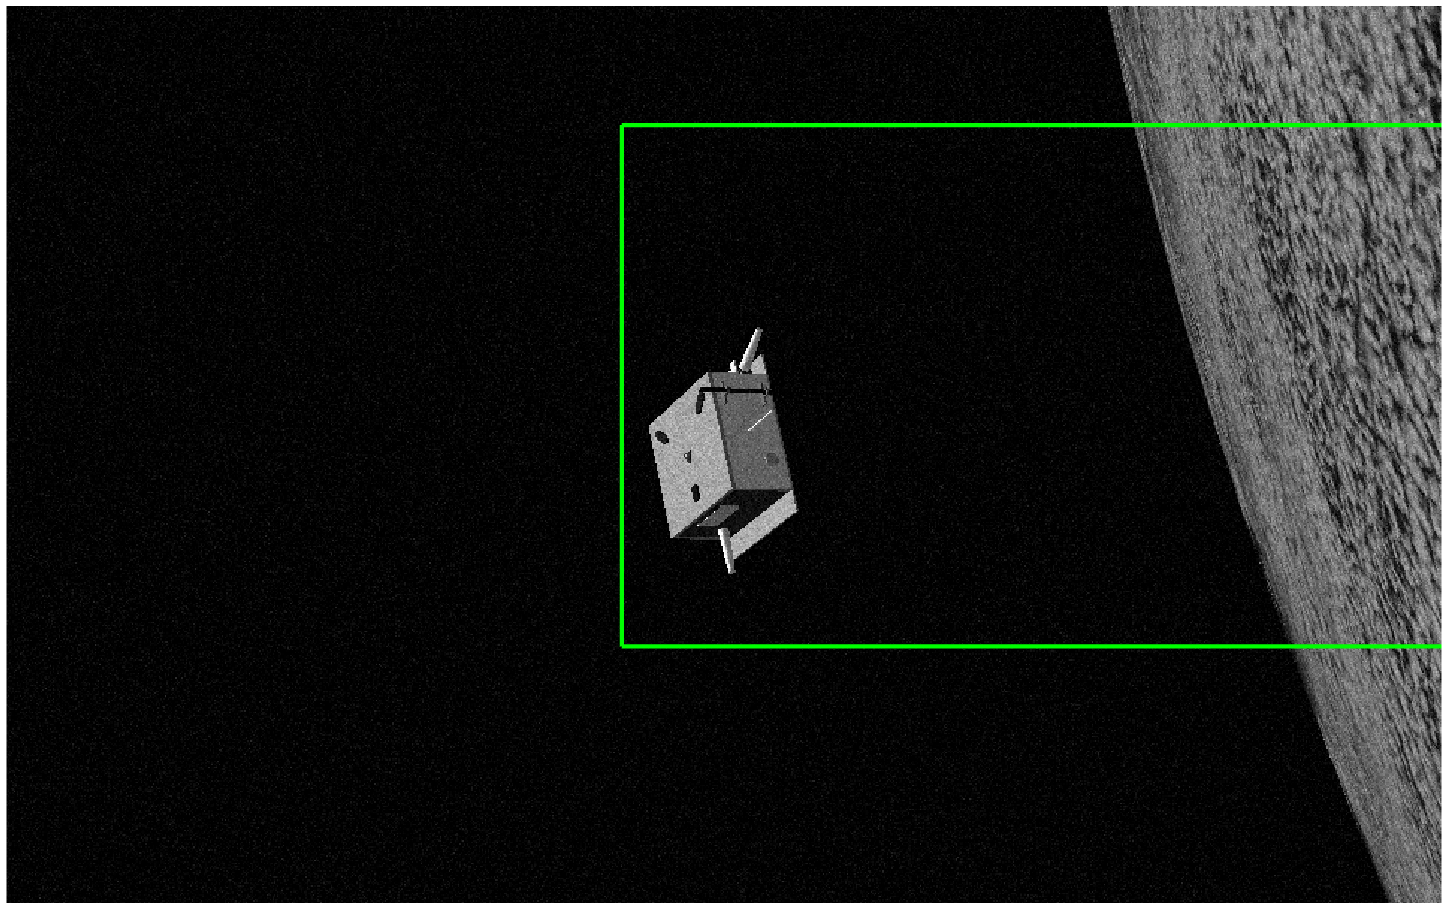
\includegraphics[width=0.47\textwidth]{gfx/results/prisma/101/9.png}}
  \qquad
  \subfloat[]{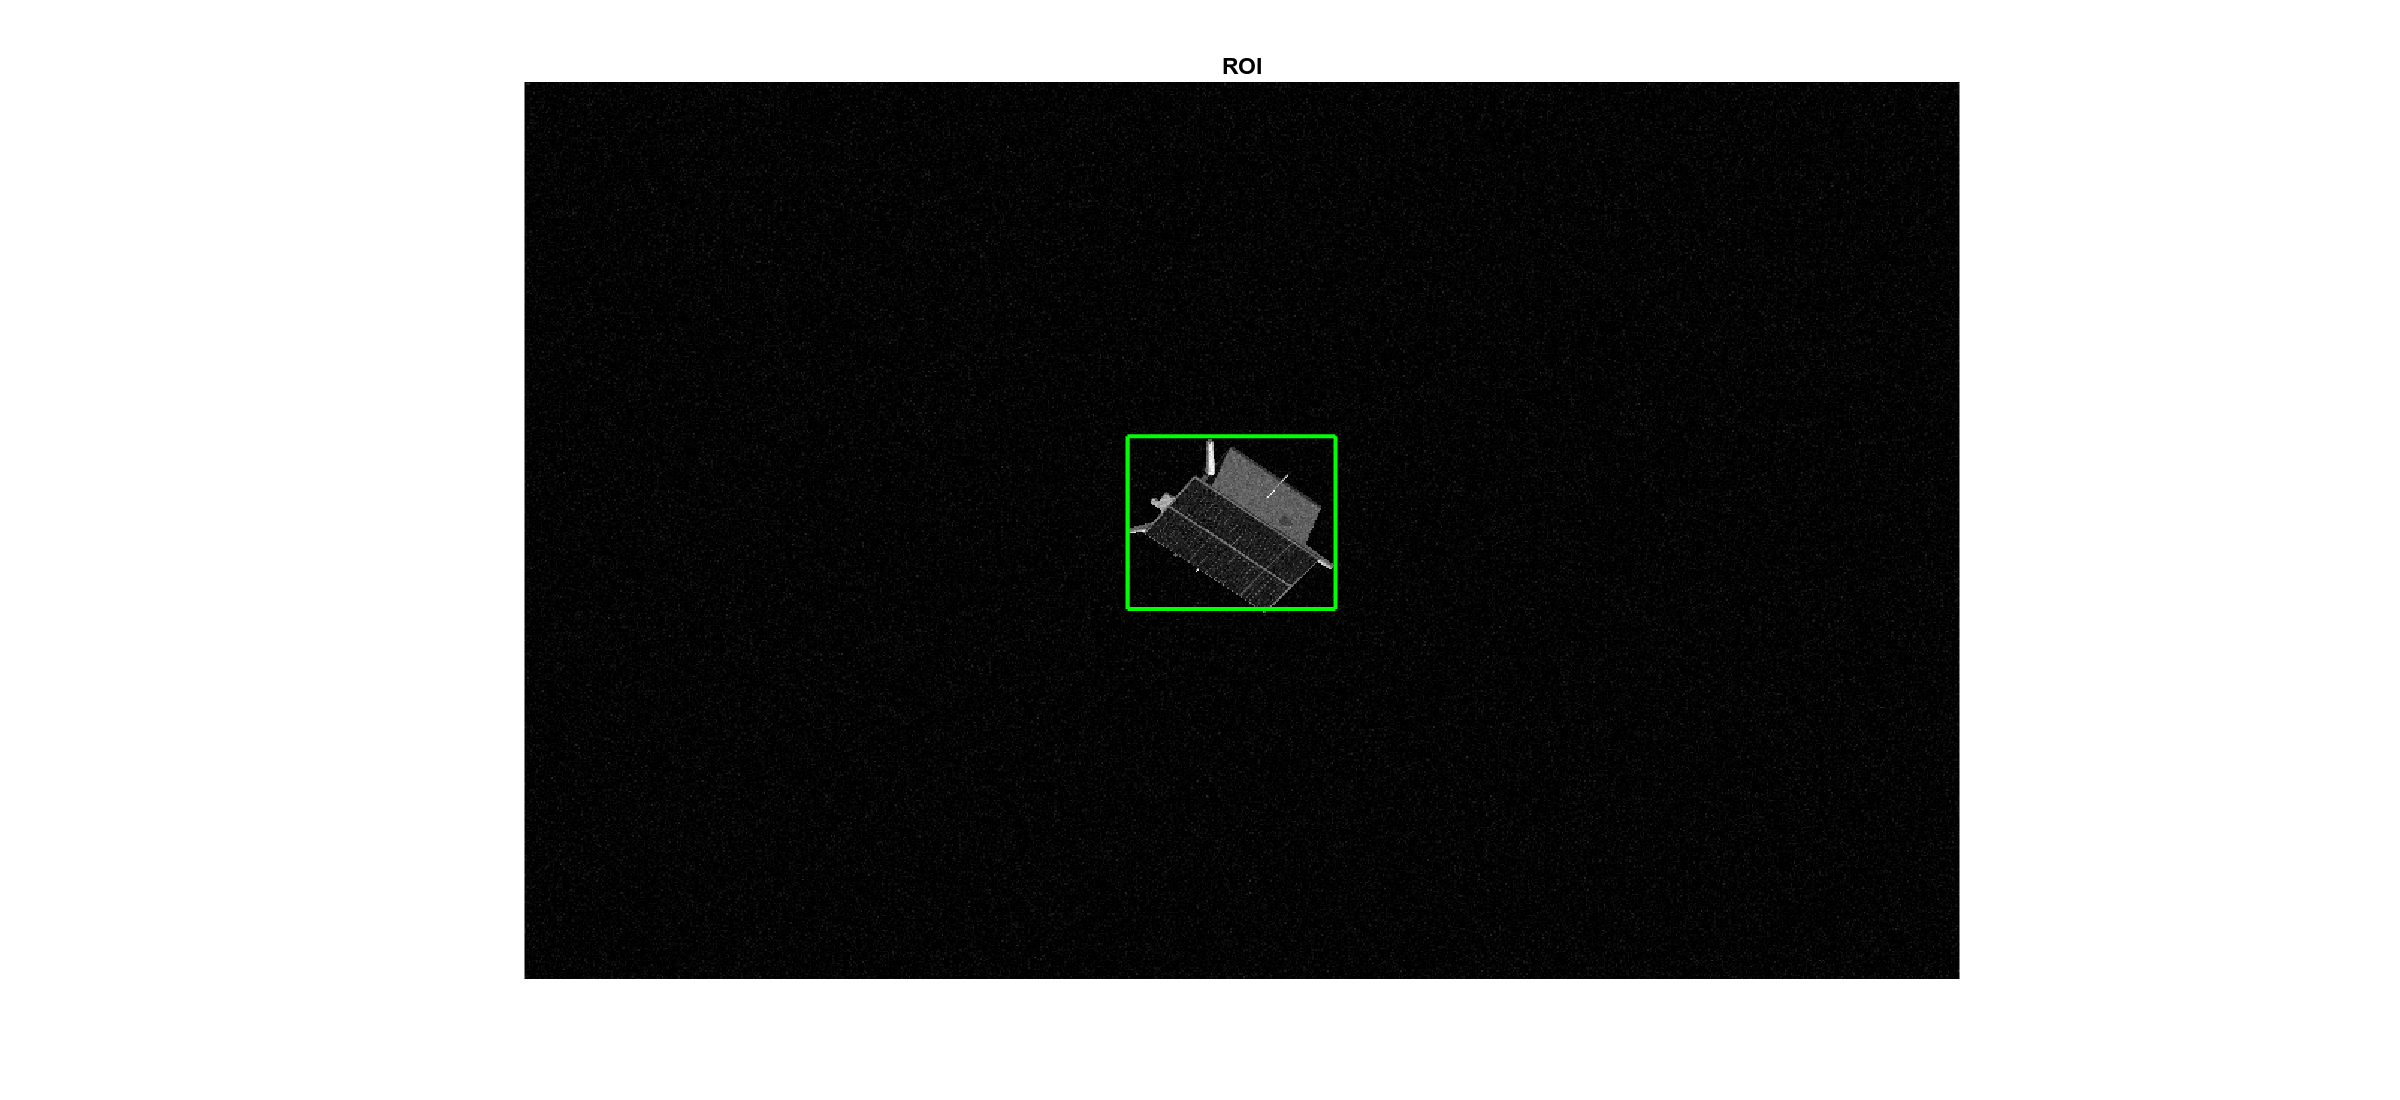
\includegraphics[width=0.47\textwidth]{gfx/results/prisma/111/9.png}}
  \qquad
  \subfloat[]{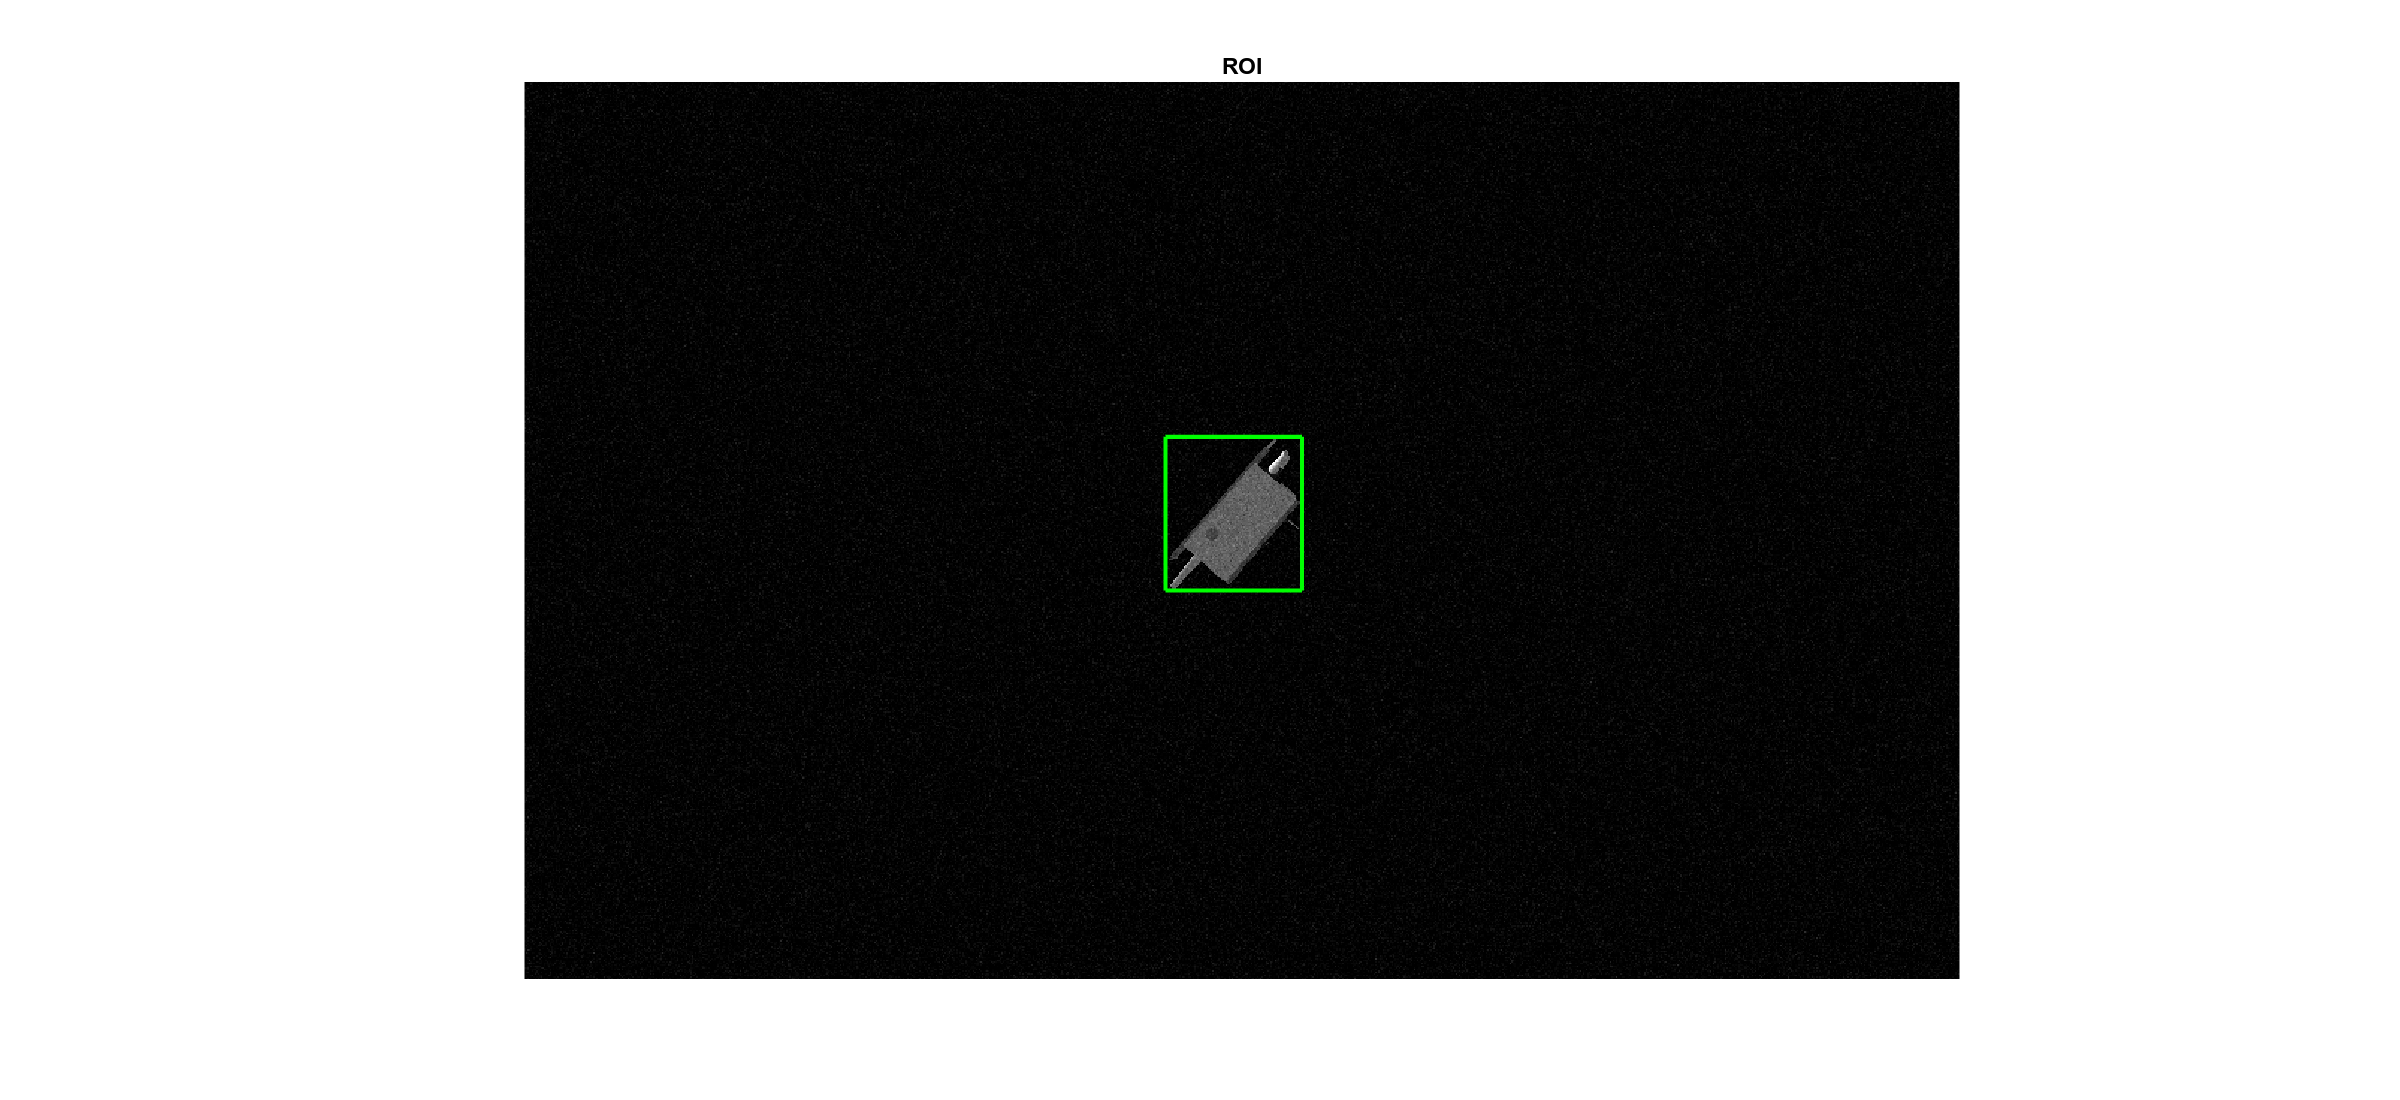
\includegraphics[width=0.47\textwidth]{gfx/results/prisma/112/9.png}}
  \qquad
  \subfloat[]{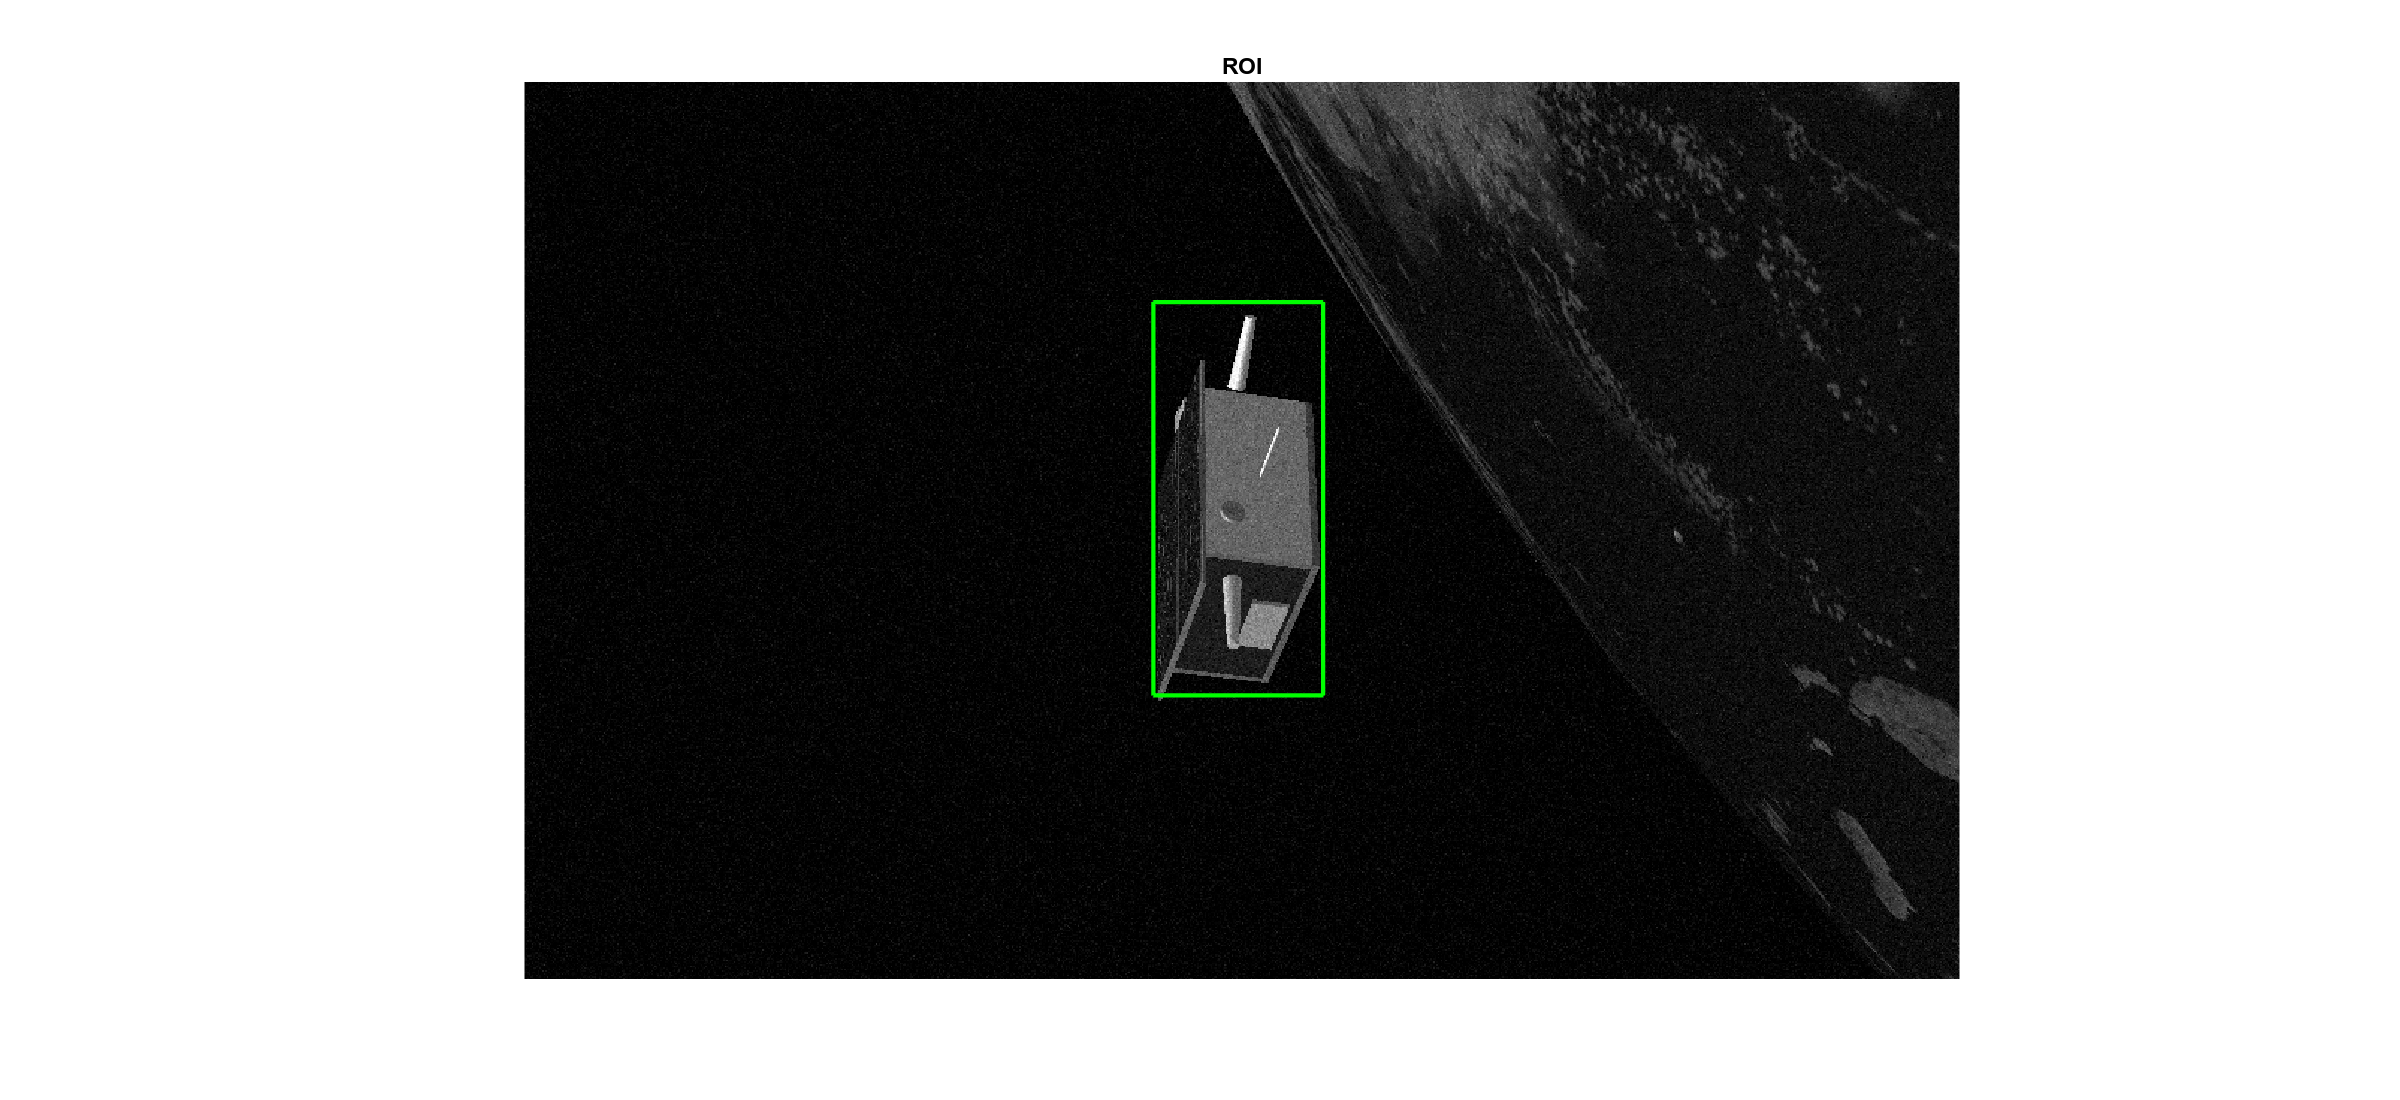
\includegraphics[width=0.47\textwidth]{gfx/results/prisma/113/9.png}}
  \qquad
  \subfloat[]{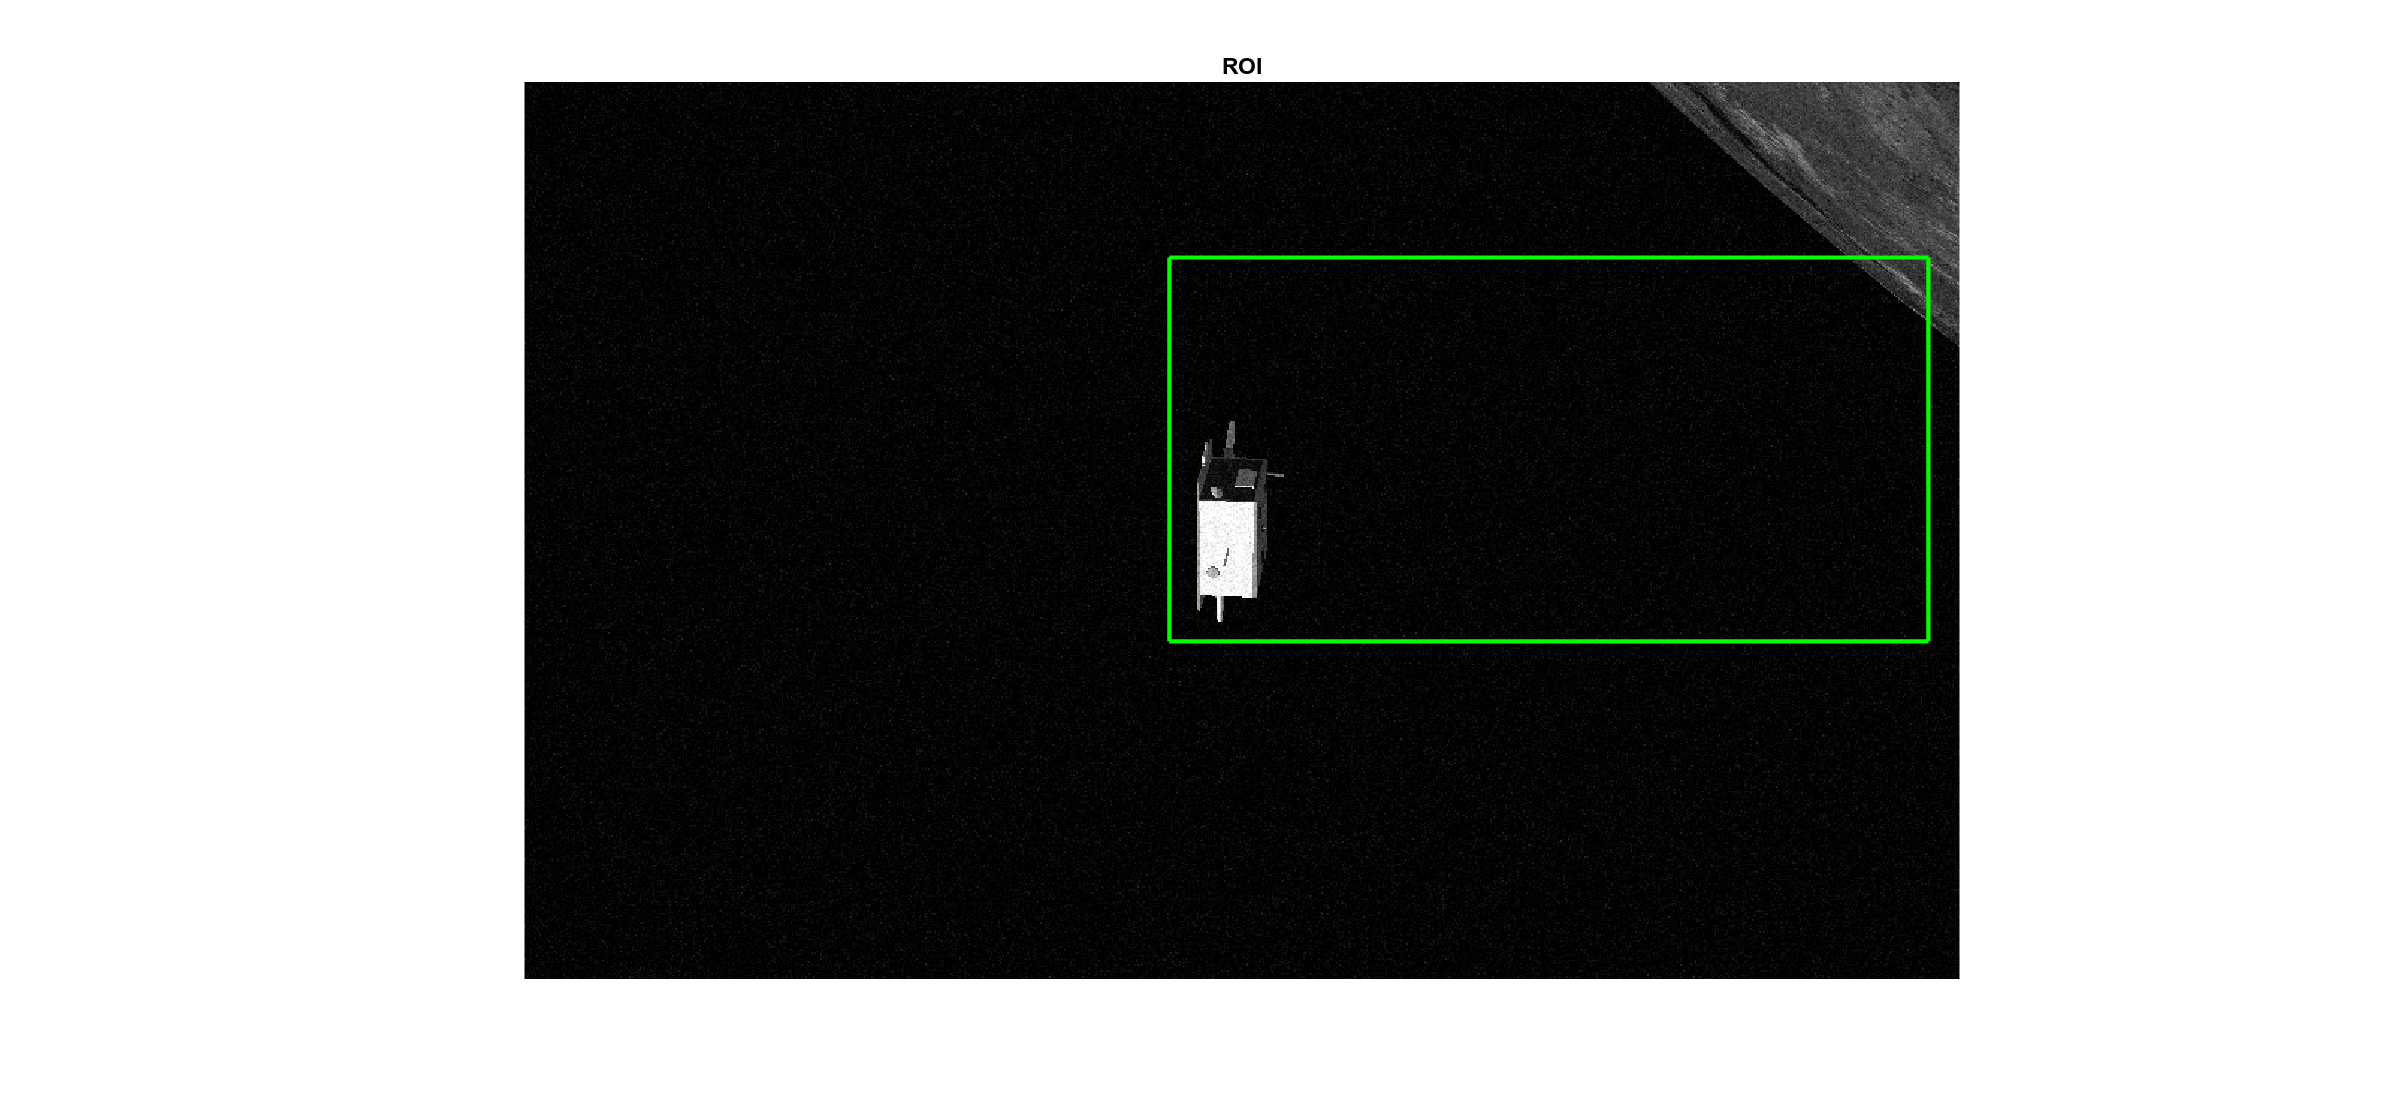
\includegraphics[width=0.47\textwidth]{gfx/results/prisma/114/9.png}}
  \qquad
  \subfloat[]{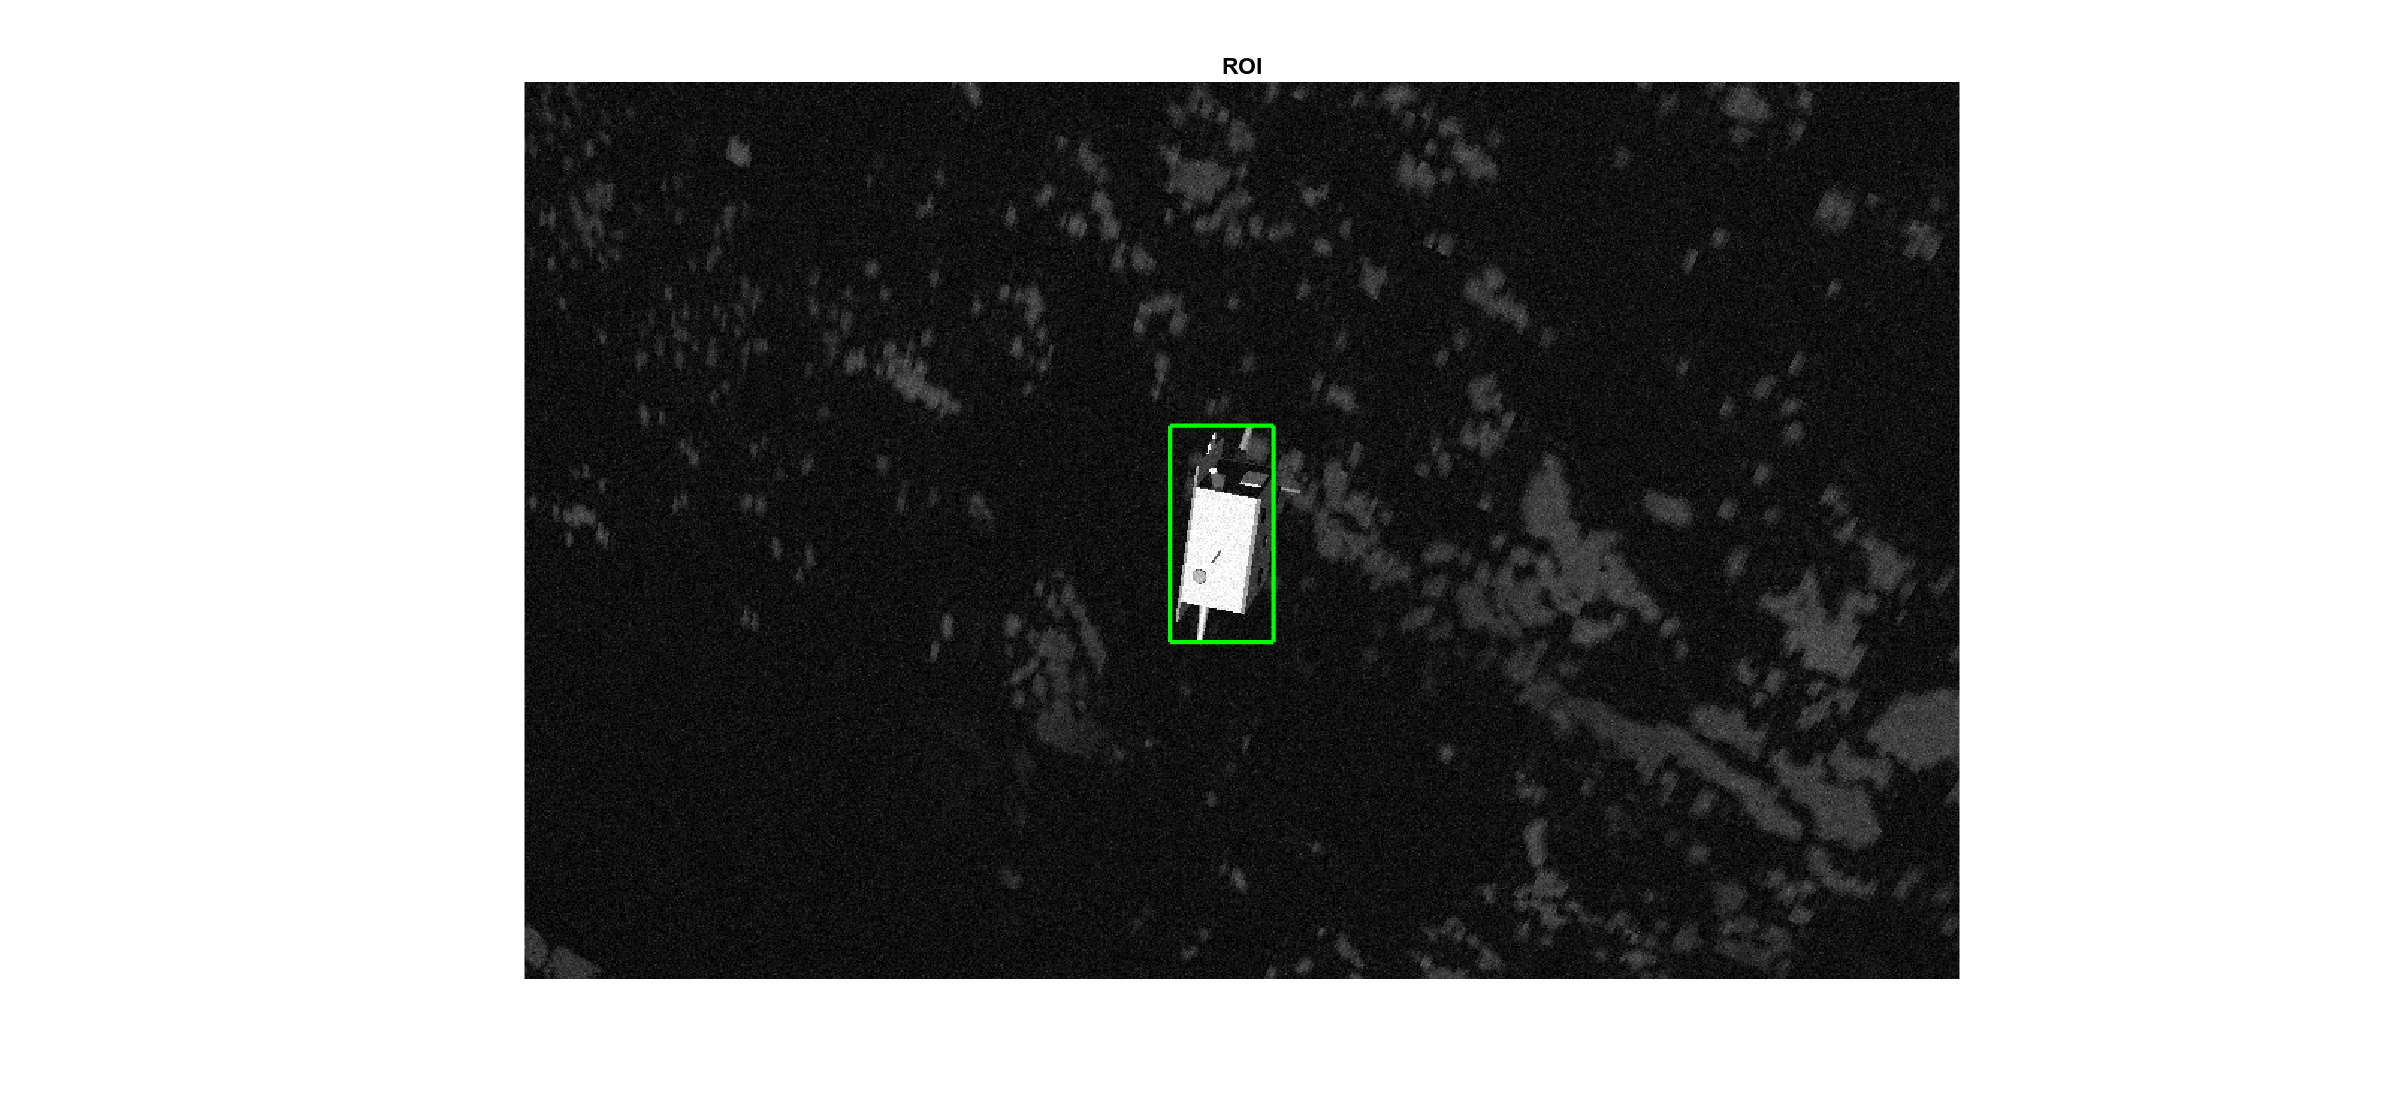
\includegraphics[width=0.47\textwidth]{gfx/results/prisma/115/9.png}}
  \qquad
  \subfloat[]{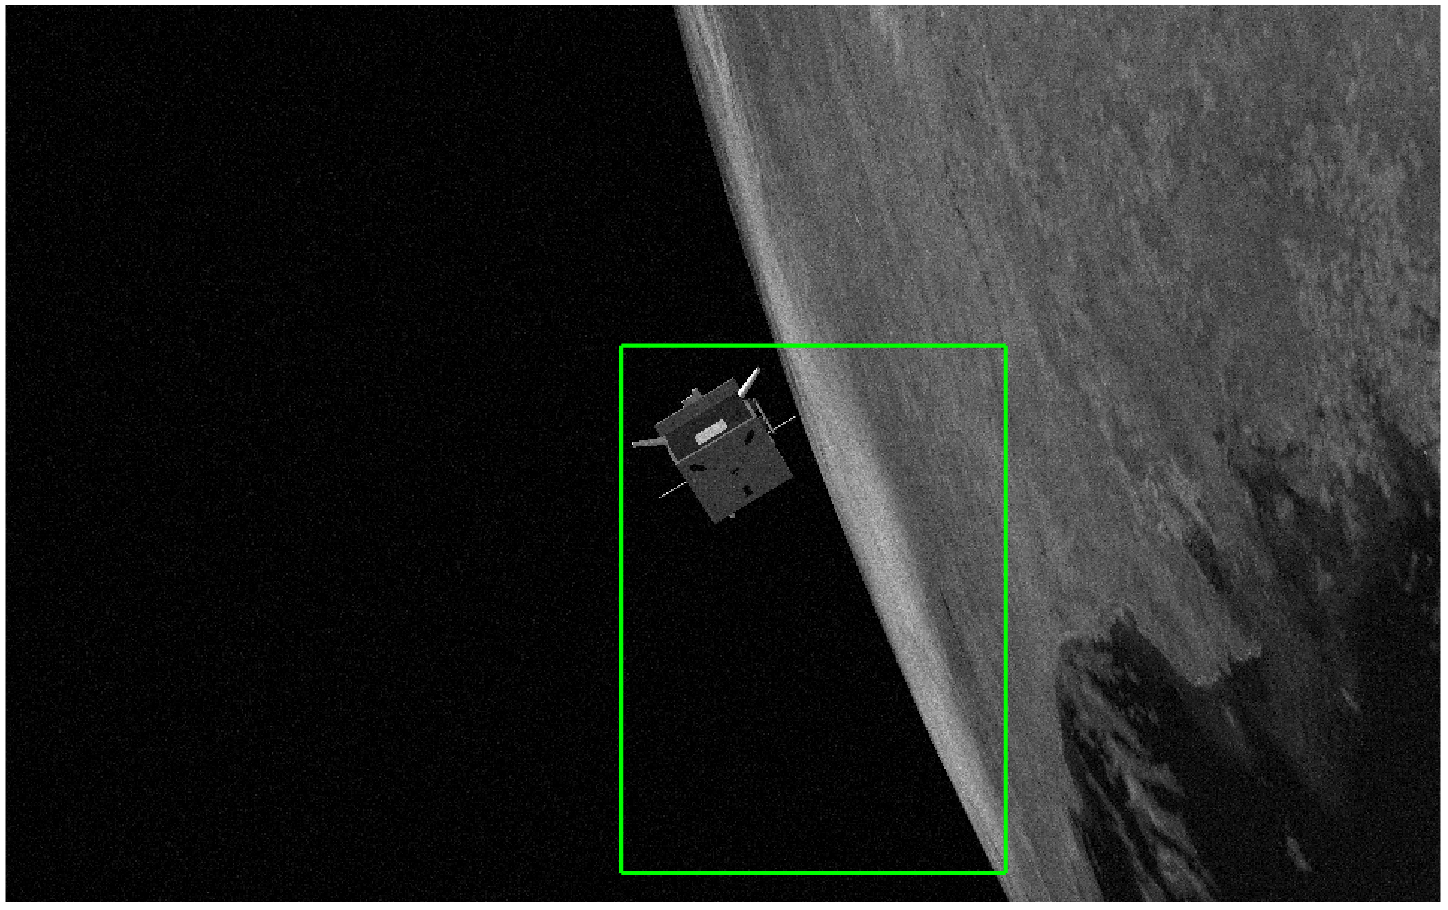
\includegraphics[width=0.47\textwidth]{gfx/results/prisma/116/9.png}}
  \qquad
  \subfloat[]{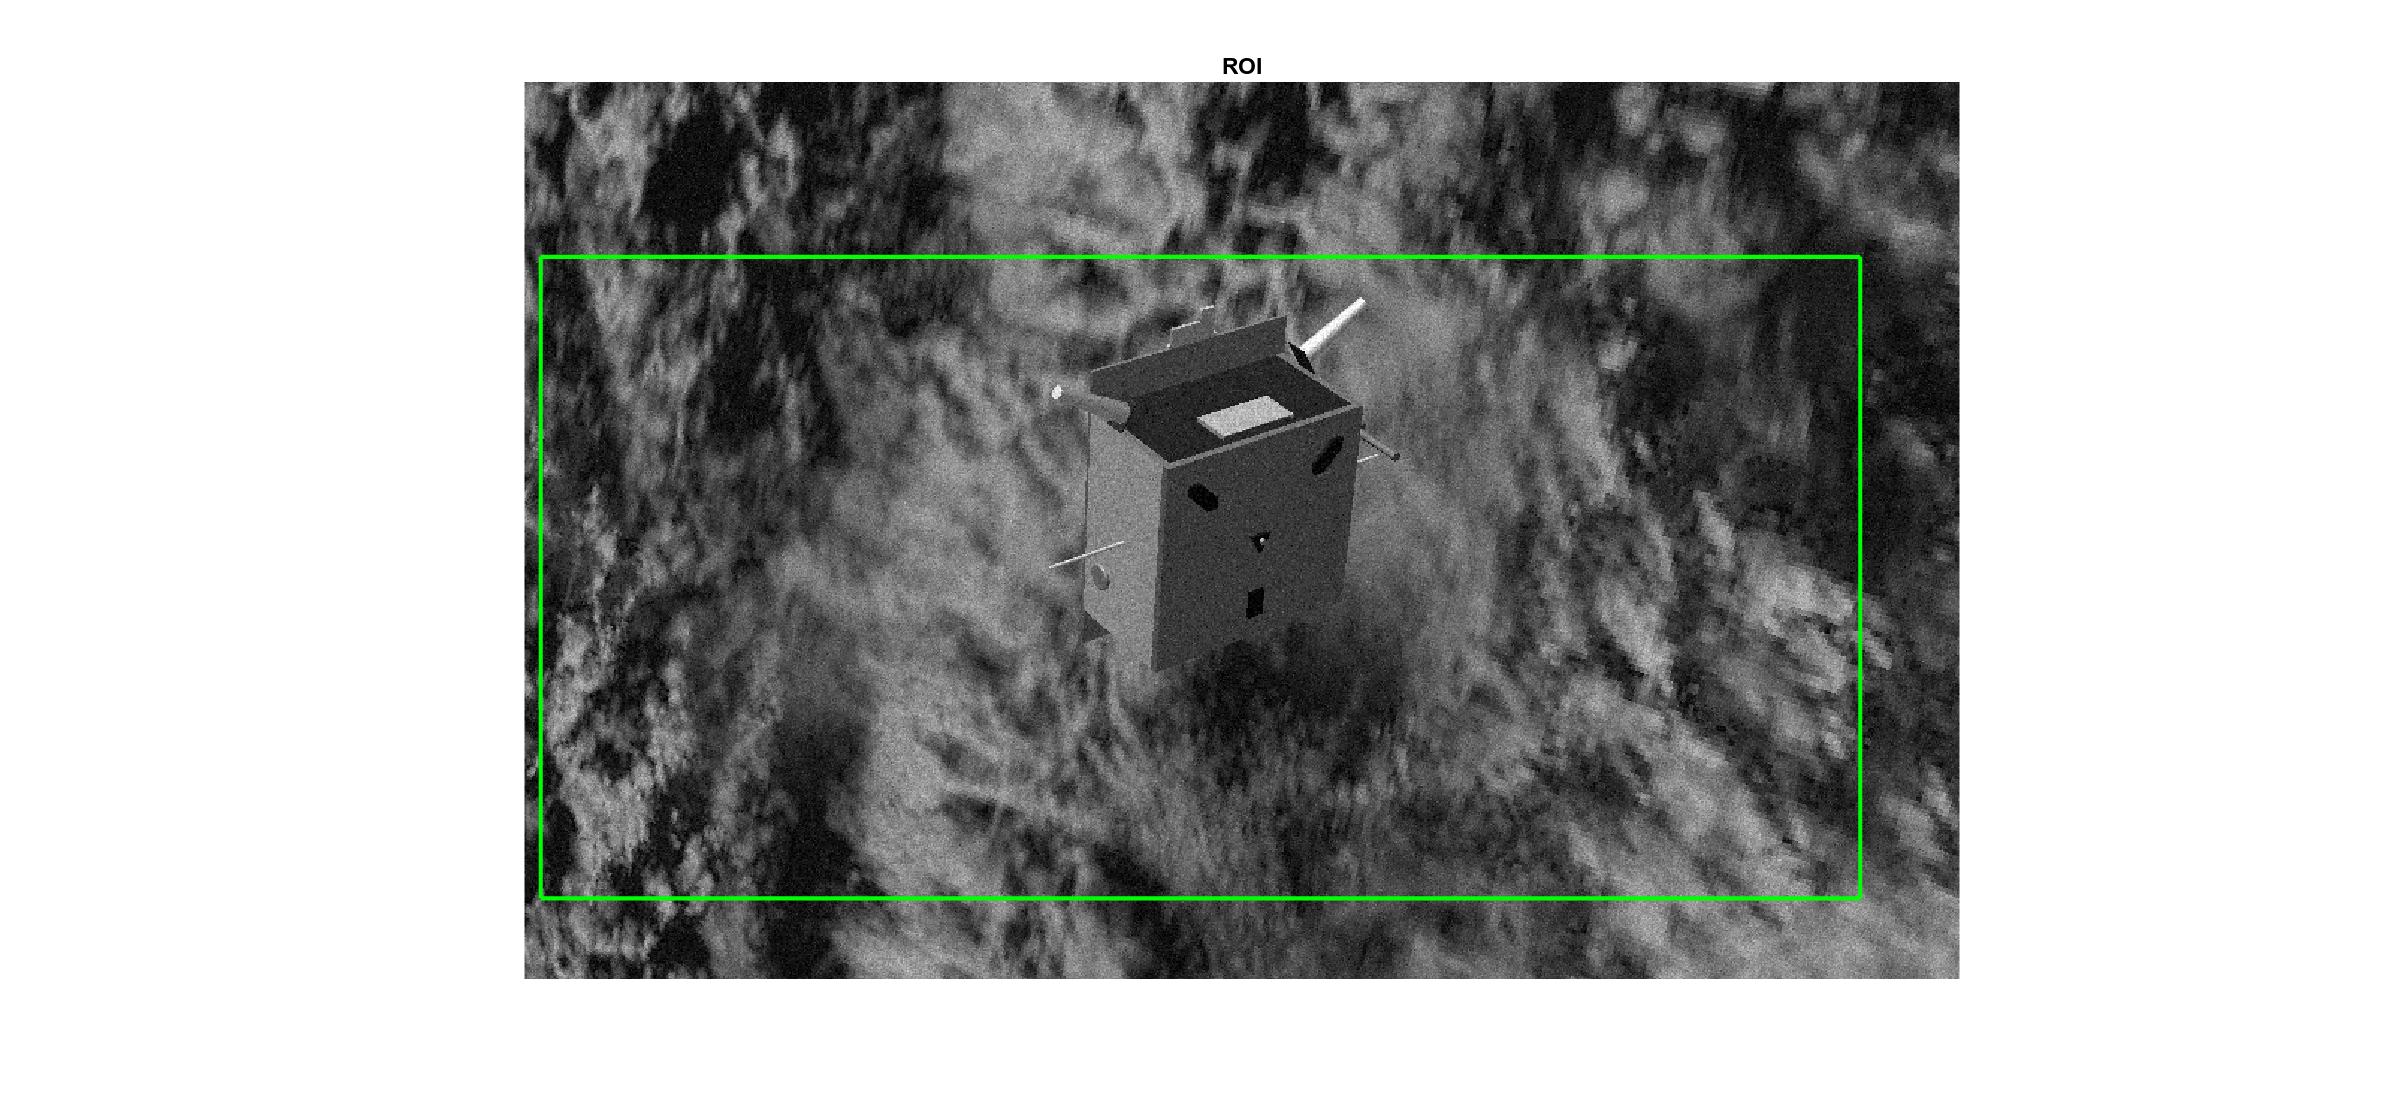
\includegraphics[width=0.47\textwidth]{gfx/results/prisma/117/9.png}}
  \qquad
  \caption{ROI detection tests.}
  \label{fig:roiResults1}
\end{figure}

\begin{figure}[htpb]
  \centering
  \subfloat[]{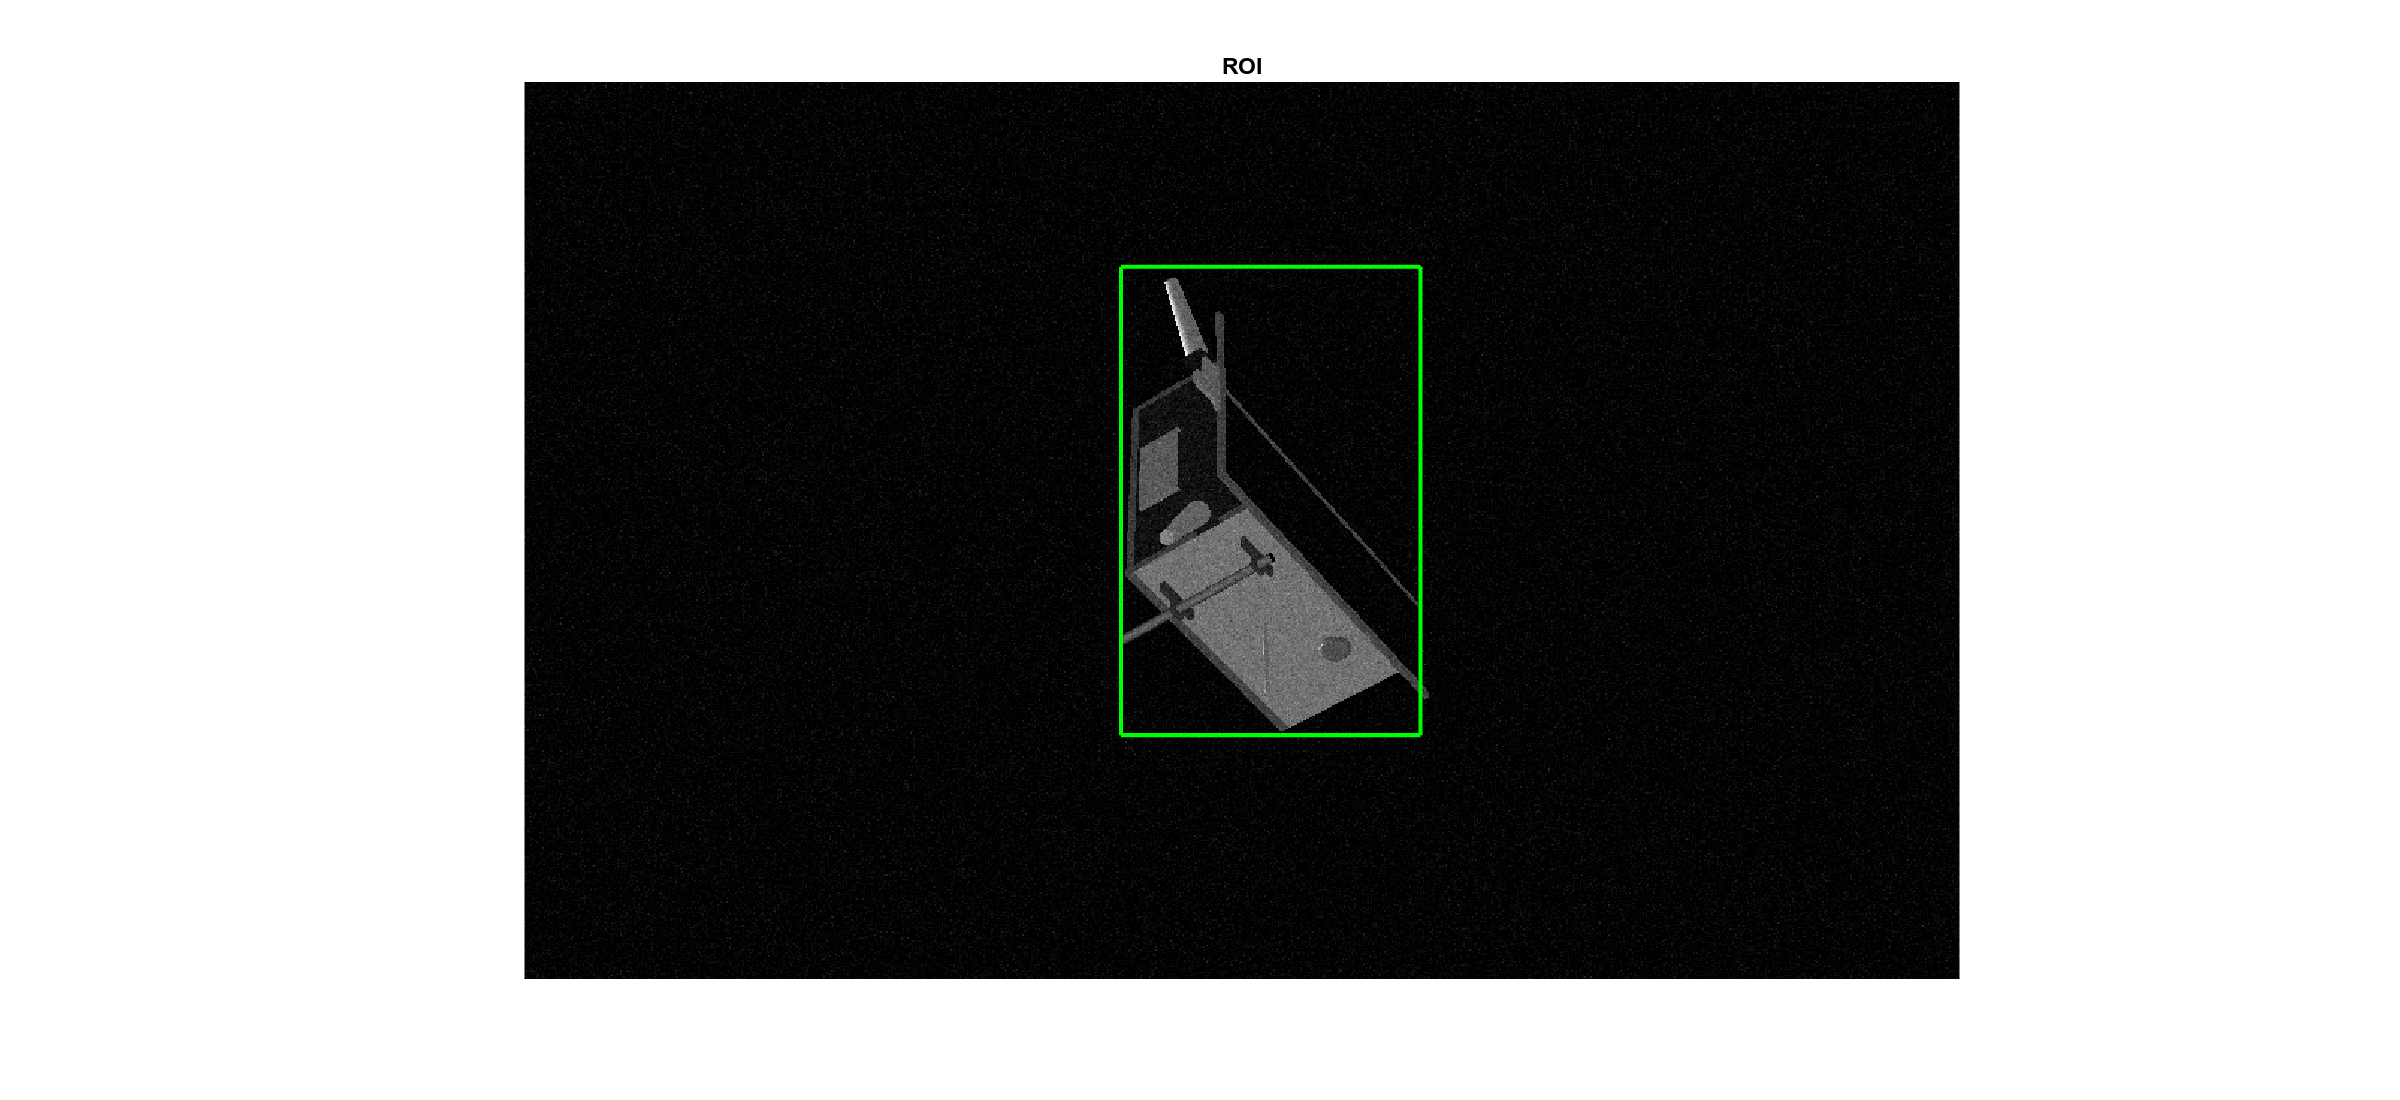
\includegraphics[width=0.47\textwidth]{gfx/results/prisma/104/9.png}}
  \qquad
  \subfloat[]{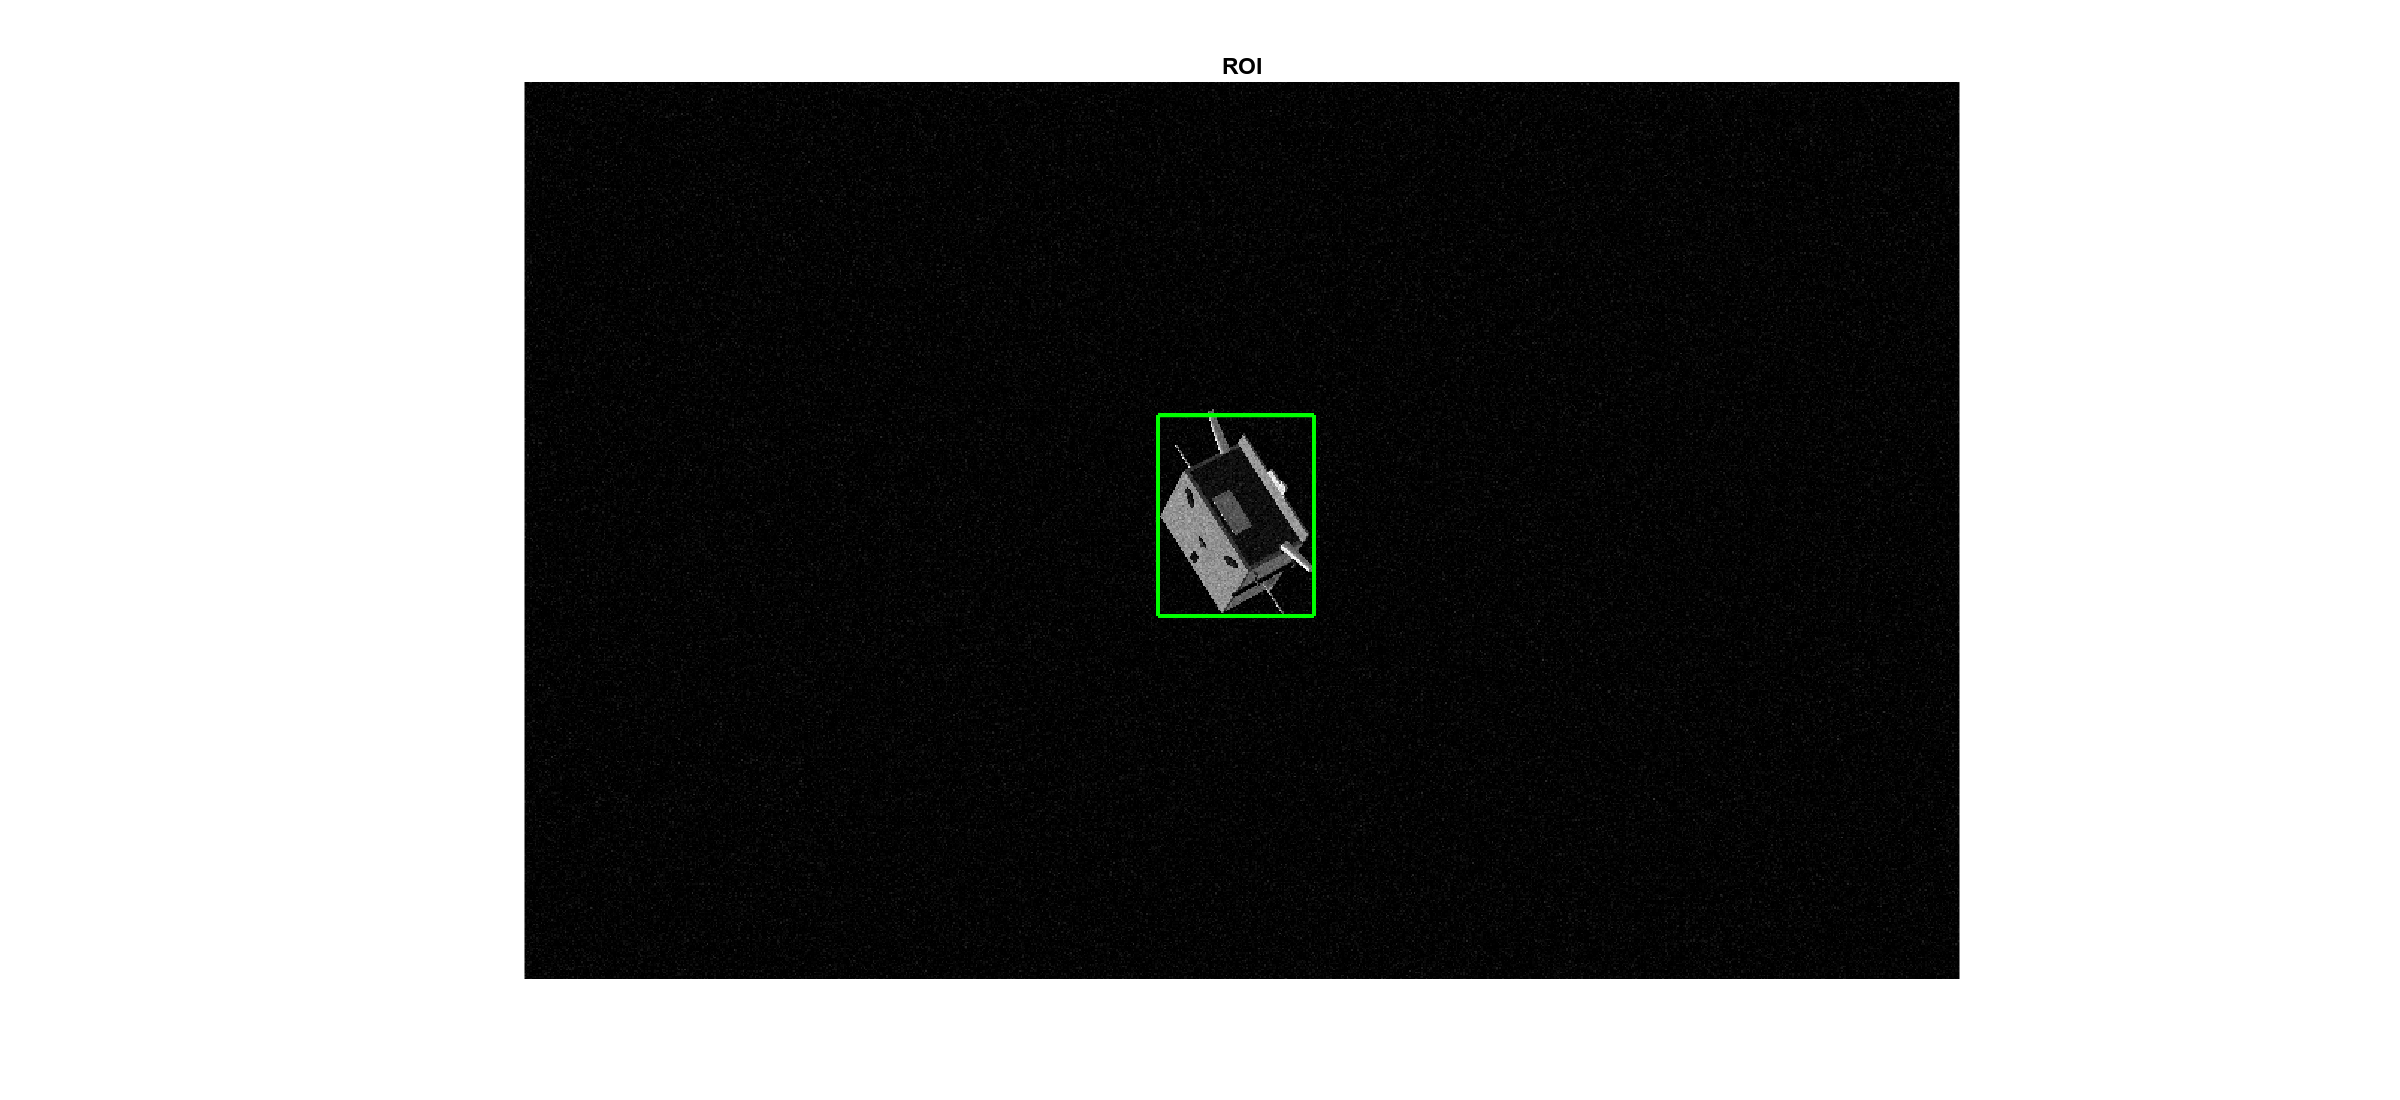
\includegraphics[width=0.47\textwidth]{gfx/results/prisma/161/9.png}}
  \qquad
  \subfloat[]{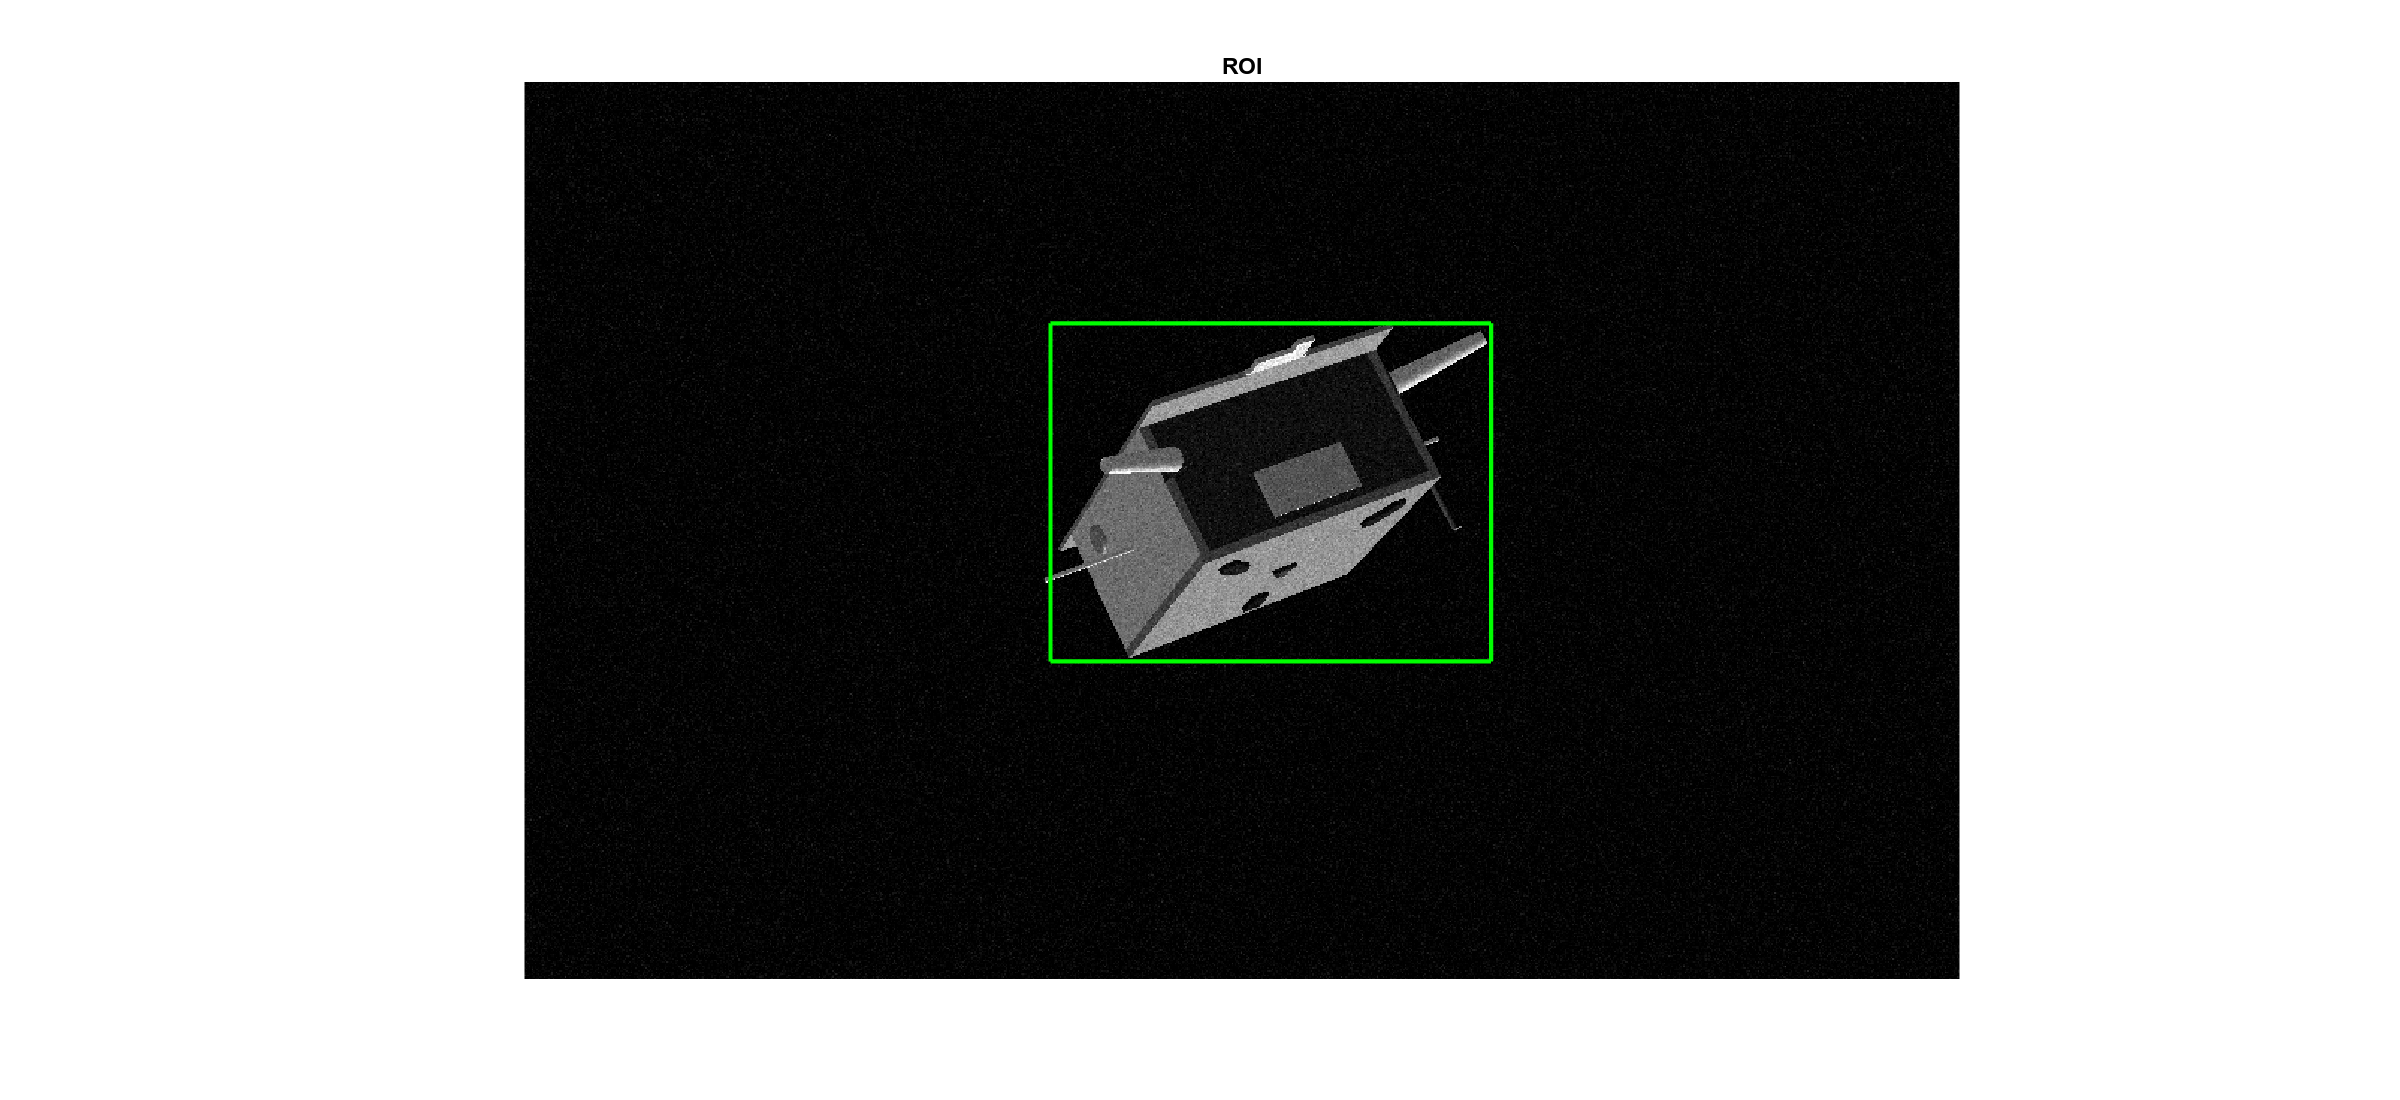
\includegraphics[width=0.47\textwidth]{gfx/results/prisma/162/9.png}}
  \qquad
  \subfloat[]{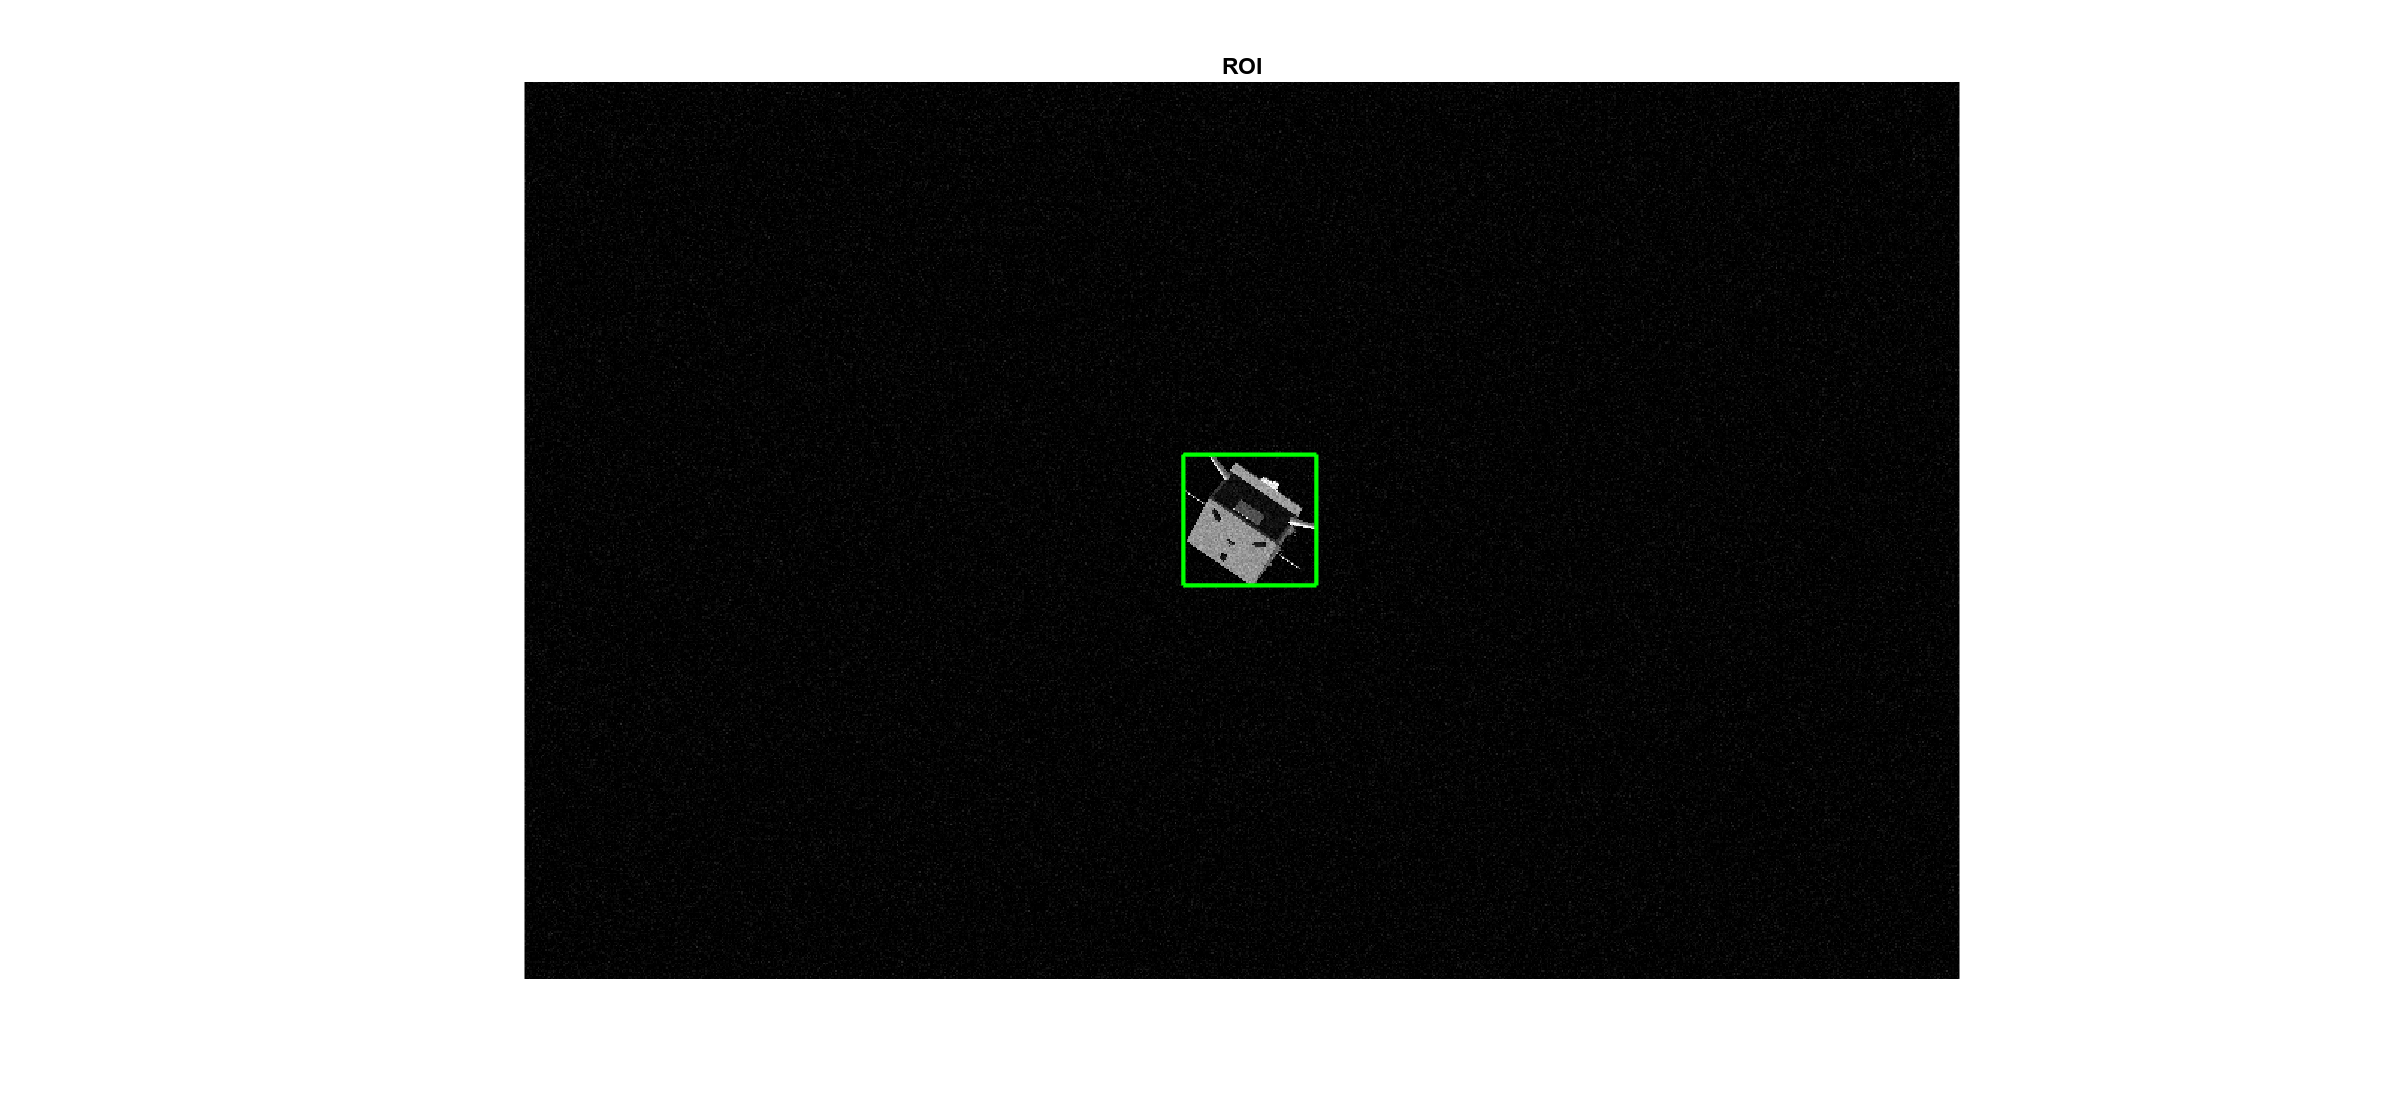
\includegraphics[width=0.47\textwidth]{gfx/results/prisma/163/9.png}}
  \qquad
  \subfloat[]{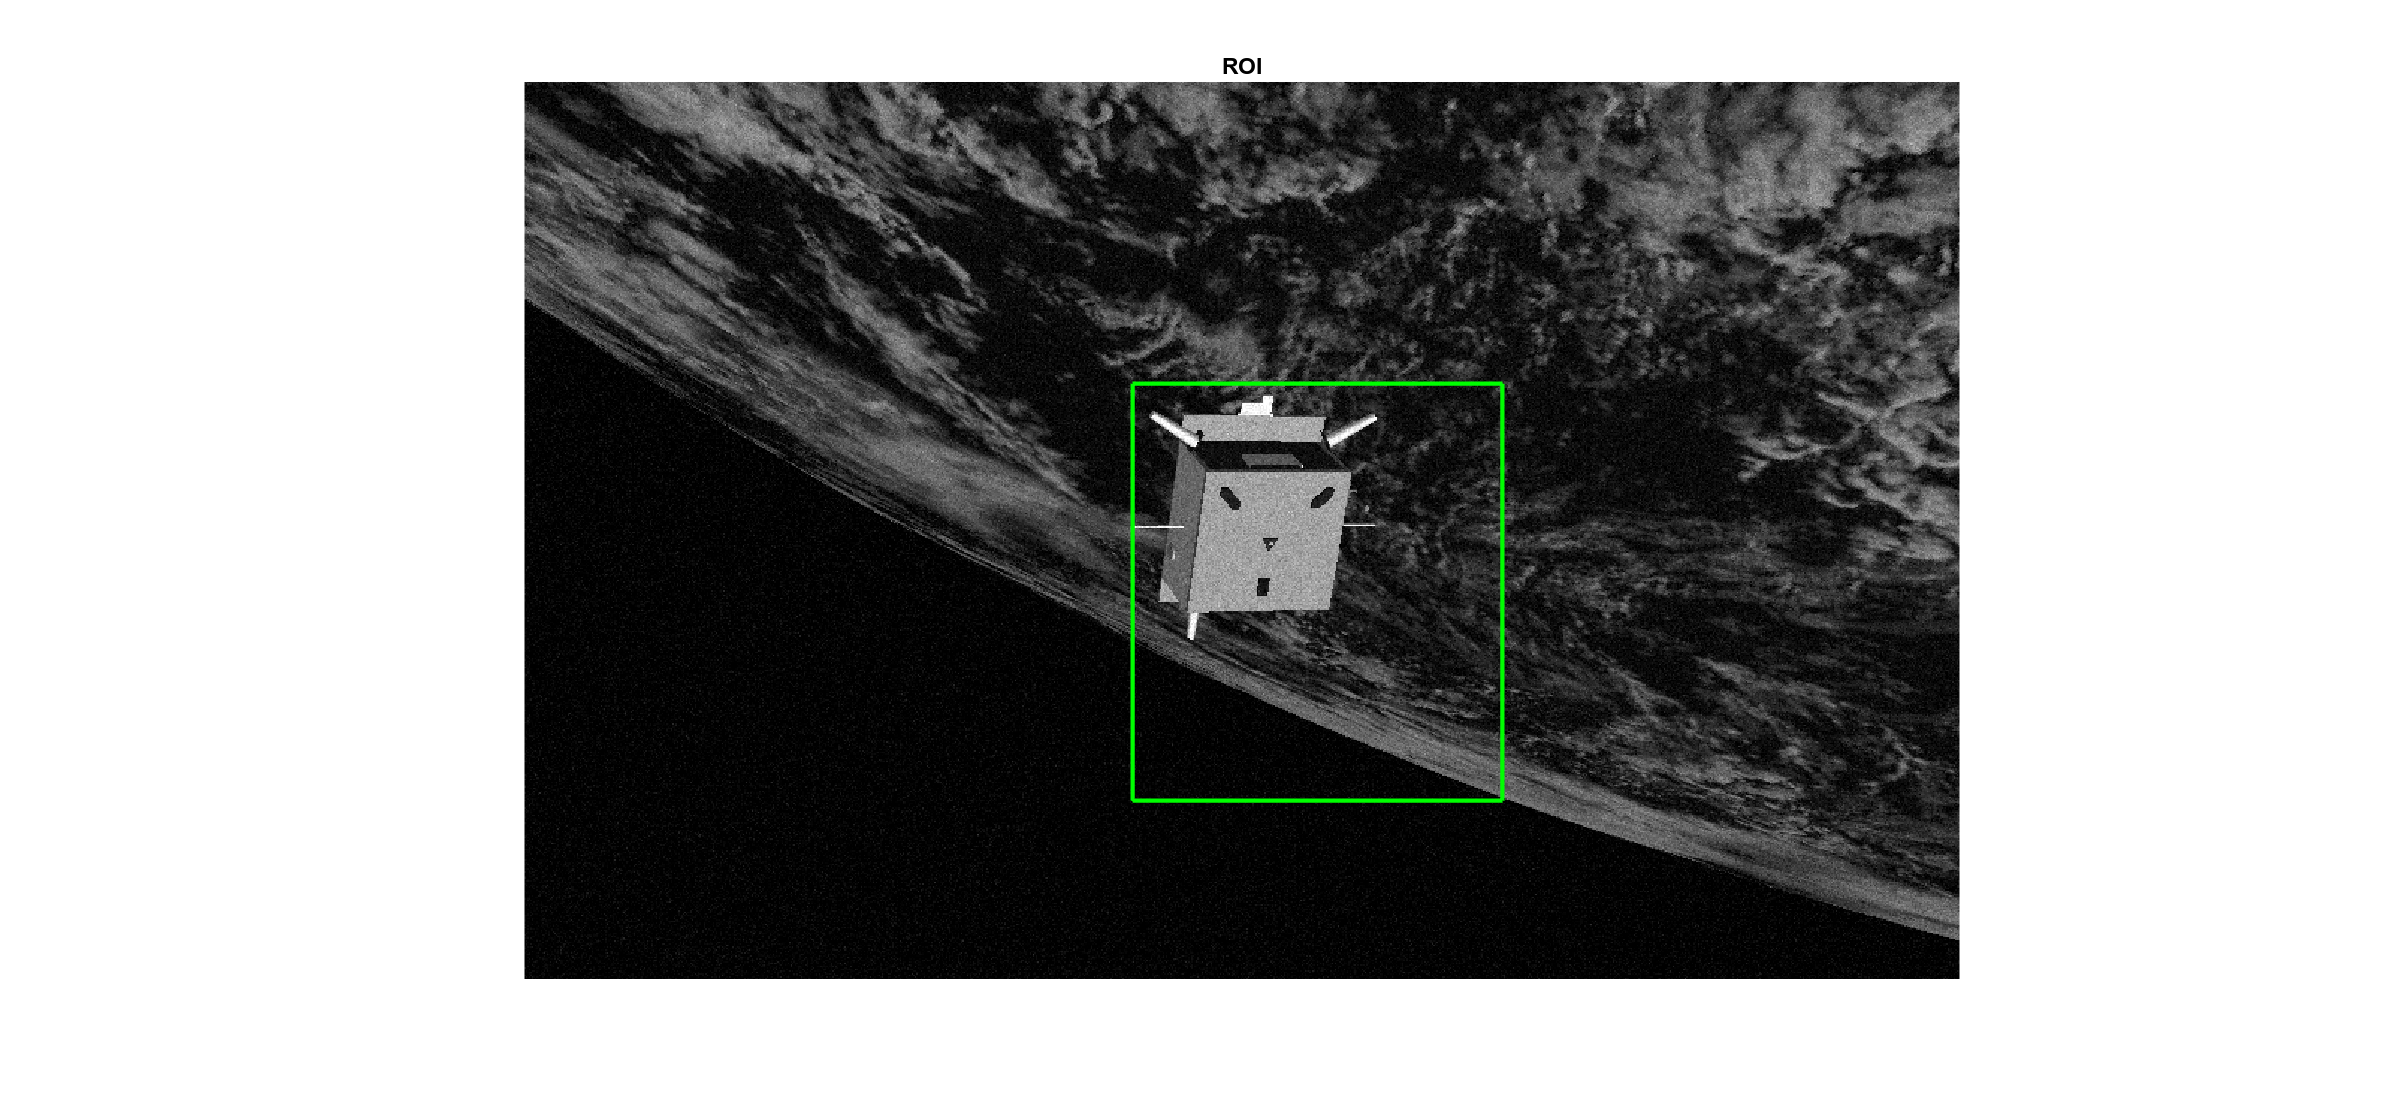
\includegraphics[width=0.47\textwidth]{gfx/results/prisma/164/9.png}}
  \qquad
  \subfloat[]{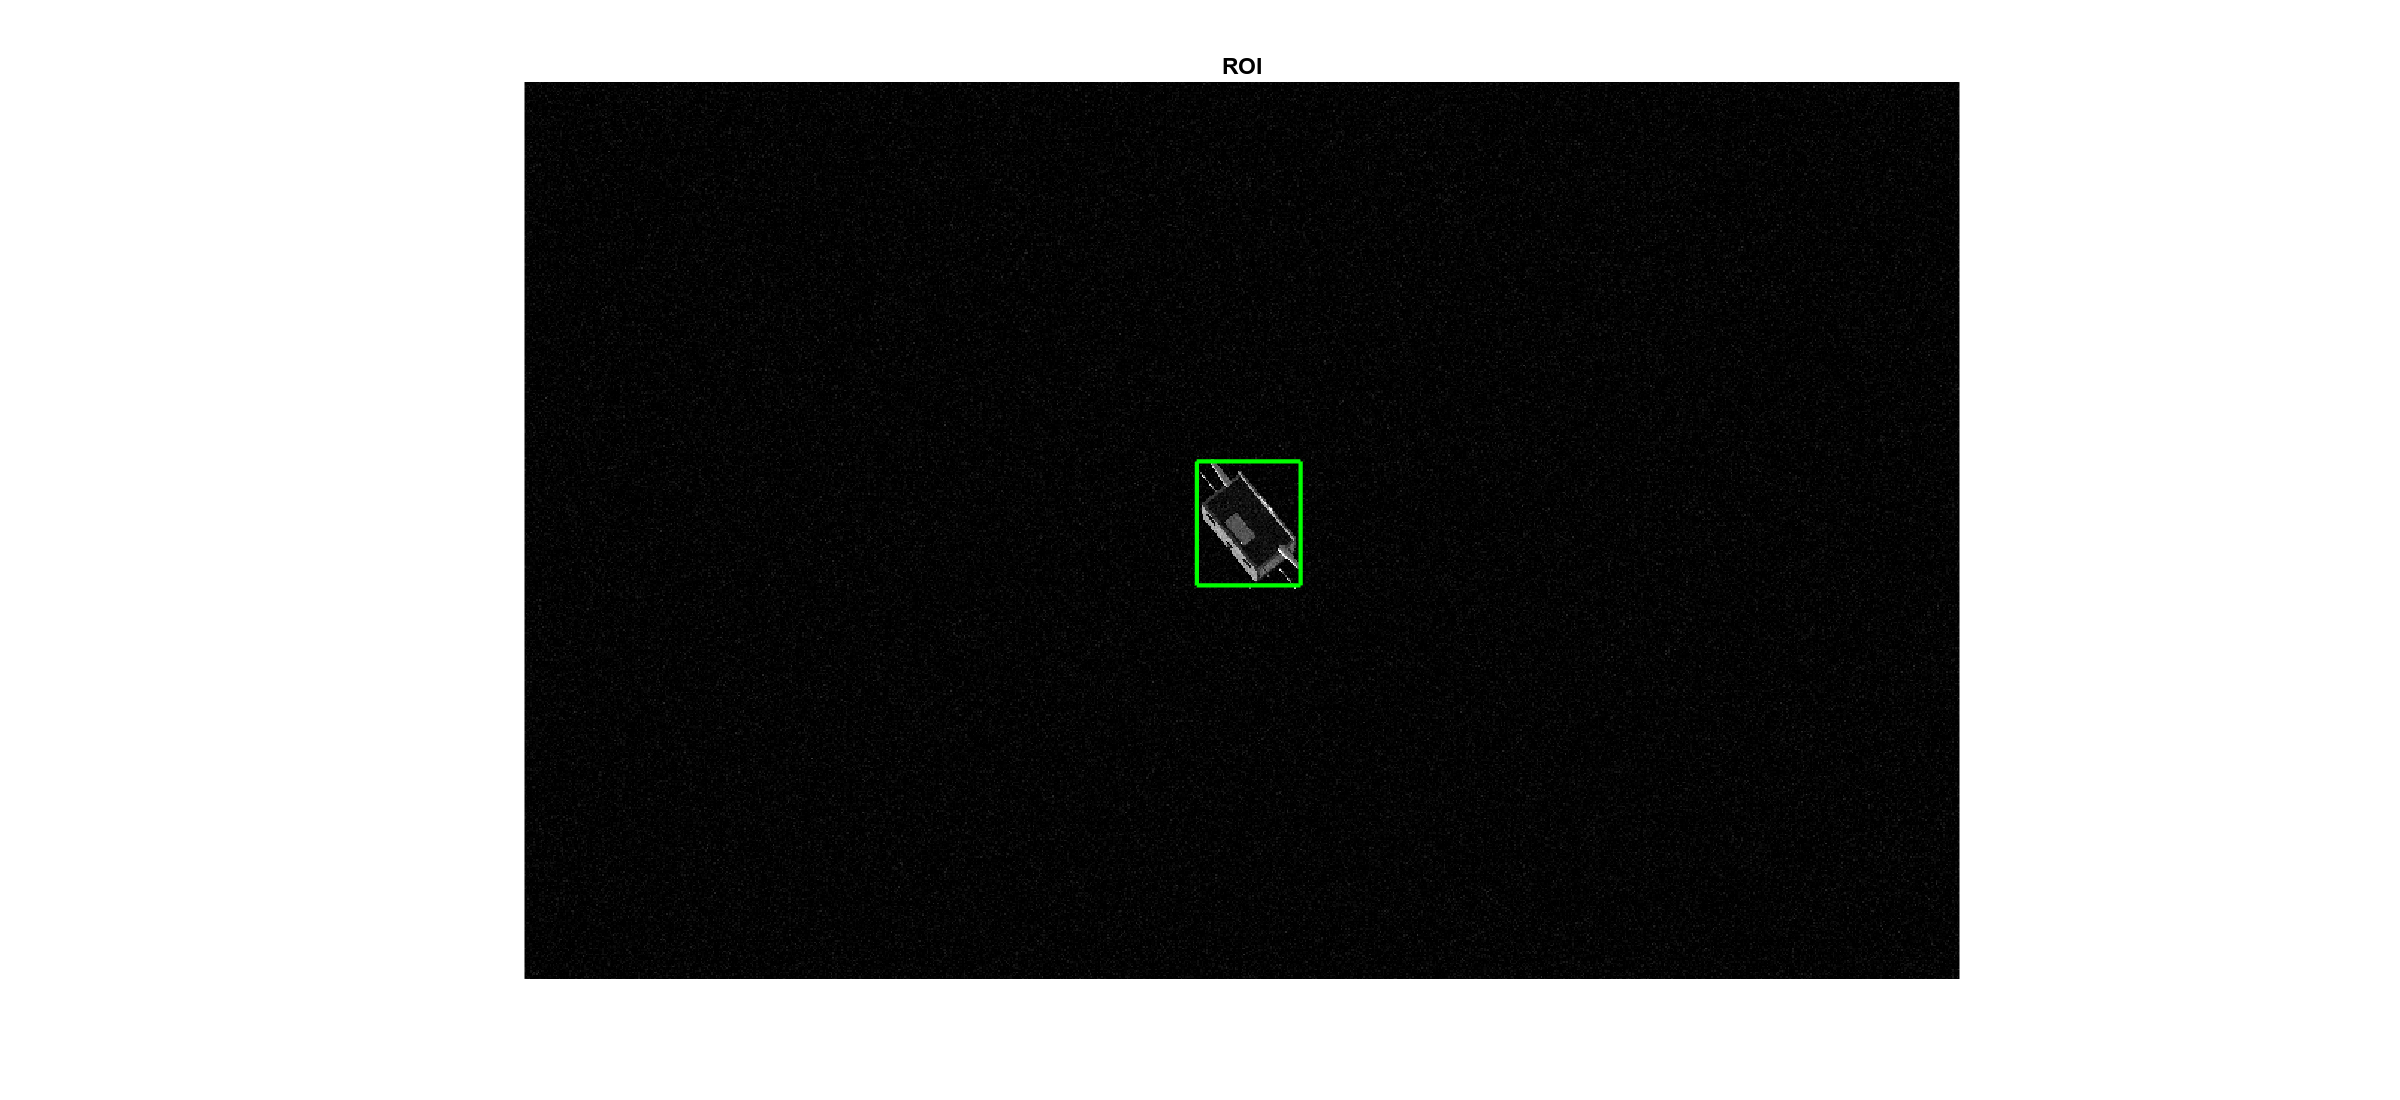
\includegraphics[width=0.47\textwidth]{gfx/results/prisma/165/9.png}}
  \qquad
  \subfloat[]{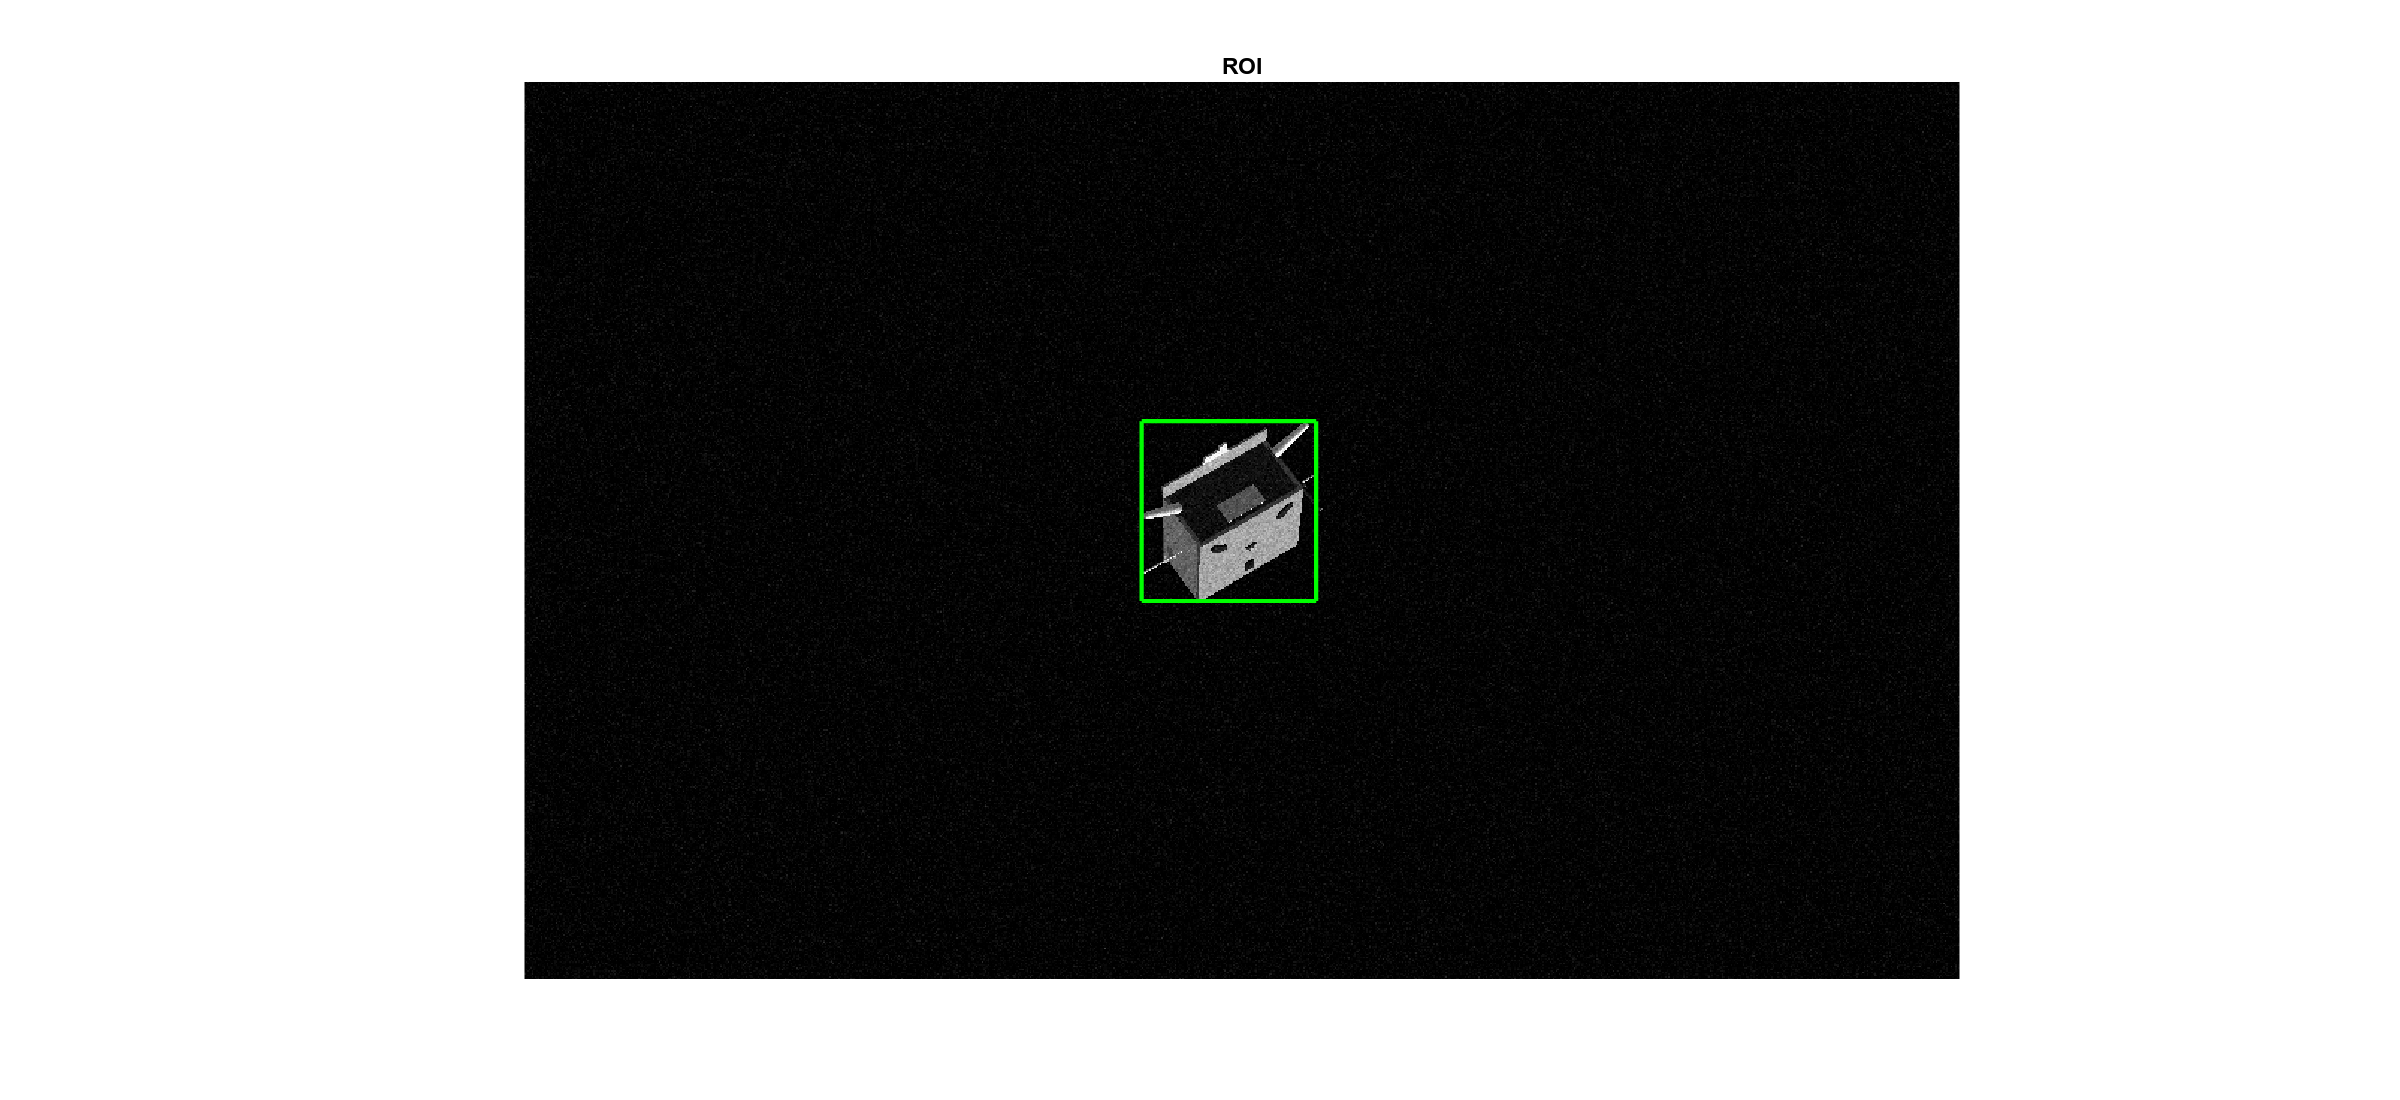
\includegraphics[width=0.47\textwidth]{gfx/results/prisma/166/9.png}}
  \qquad
  \subfloat[]{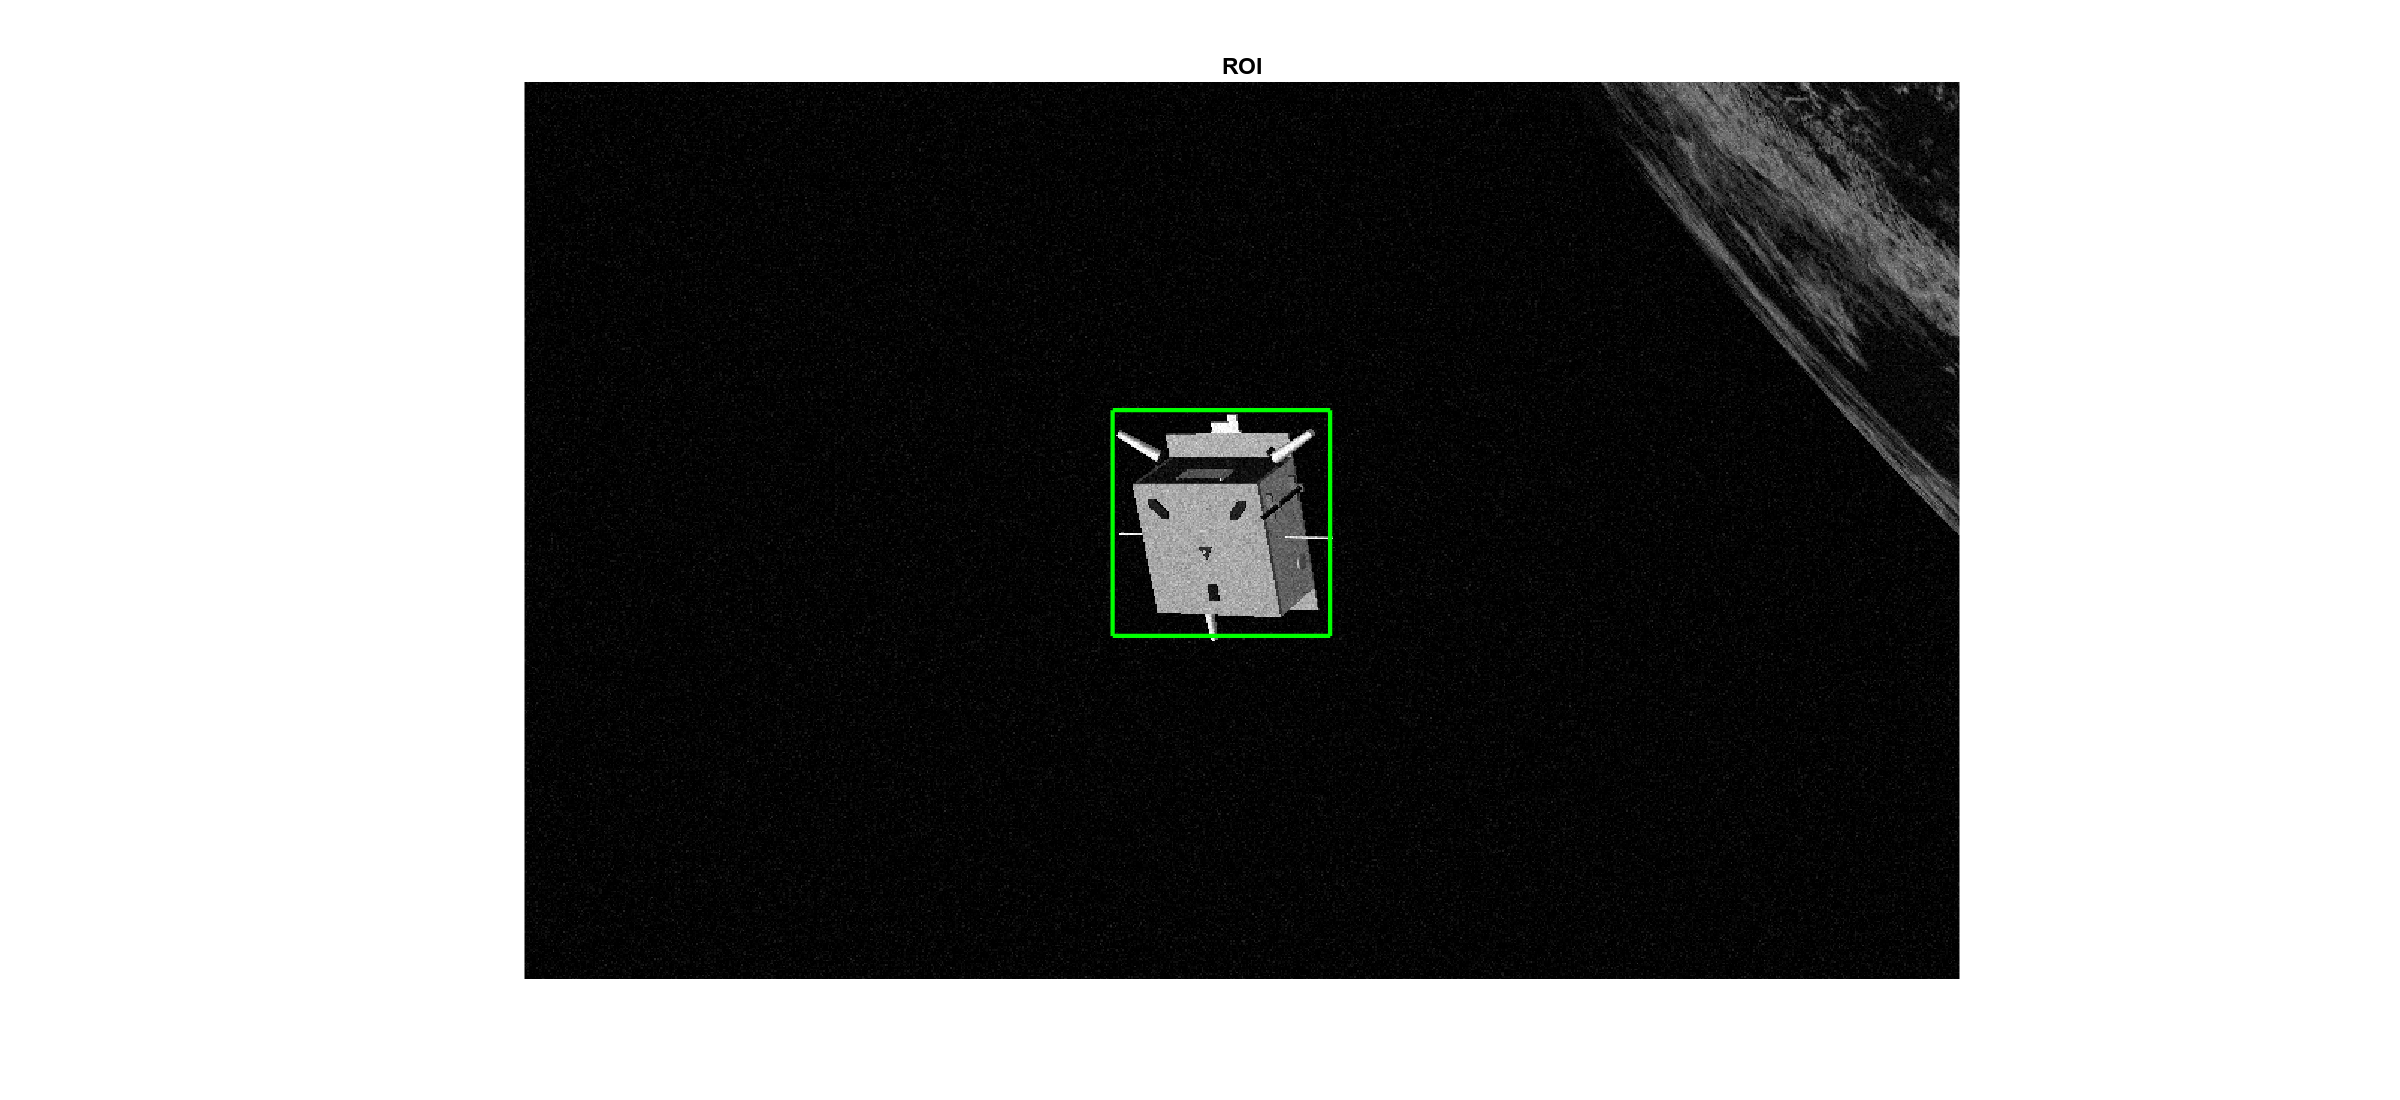
\includegraphics[width=0.47\textwidth]{gfx/results/prisma/169/9.png}}
  \qquad
  \caption{ROI detection tests.}
  \label{fig:roiResults2}
\end{figure}

\begin{figure}[htpb]
  \centering
  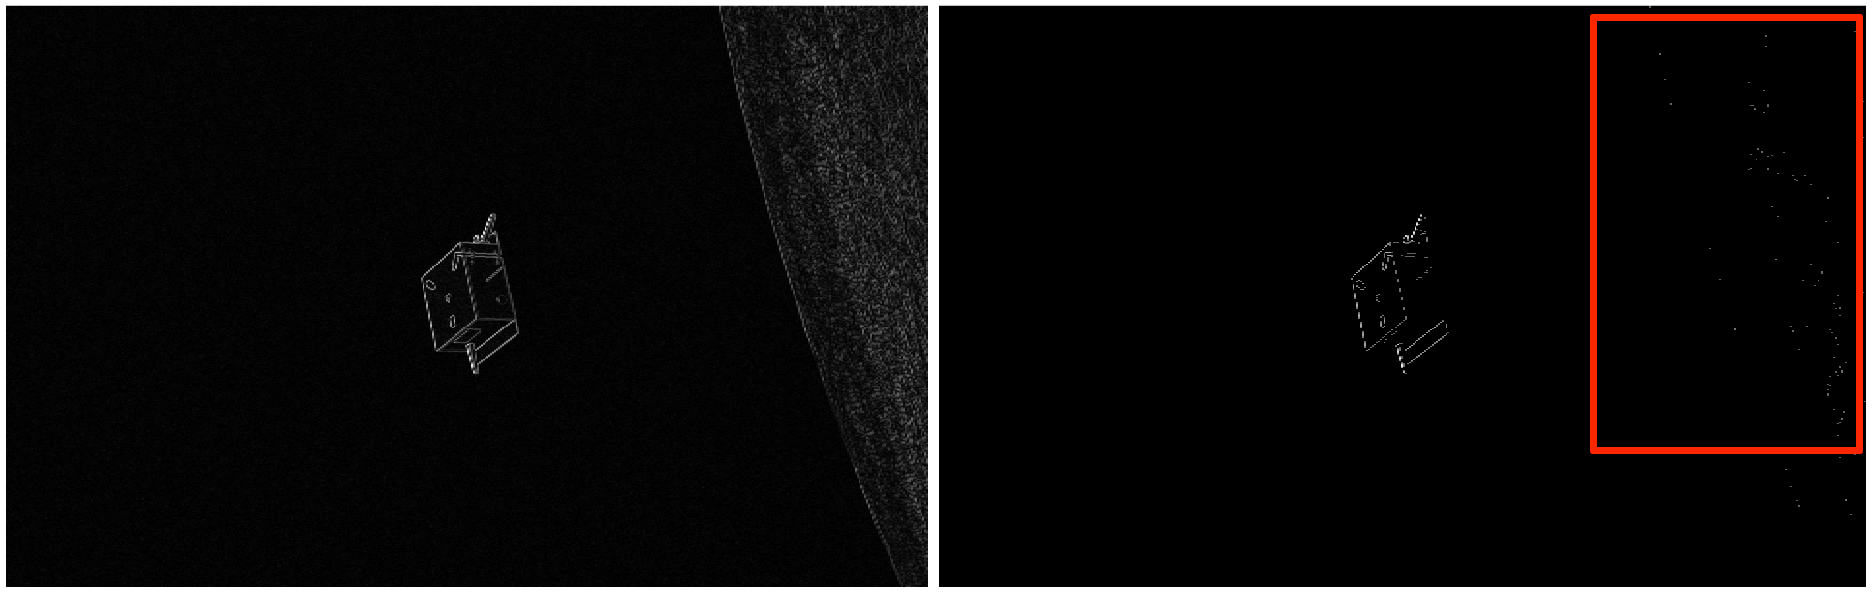
\includegraphics[width=1.0\textwidth]{gfx/results/prisma/101/8Select.png}
  \caption{Gradient image of Figure~\ref{fig:roiResults1}a. Left is normalized gradient, right is normalized gradient after tresholding. The spurious points not filtered by the \acrshort{wge} technique are enclosed in the red box.}
\end{figure}

\begin{figure}[htpb]
  \centering
  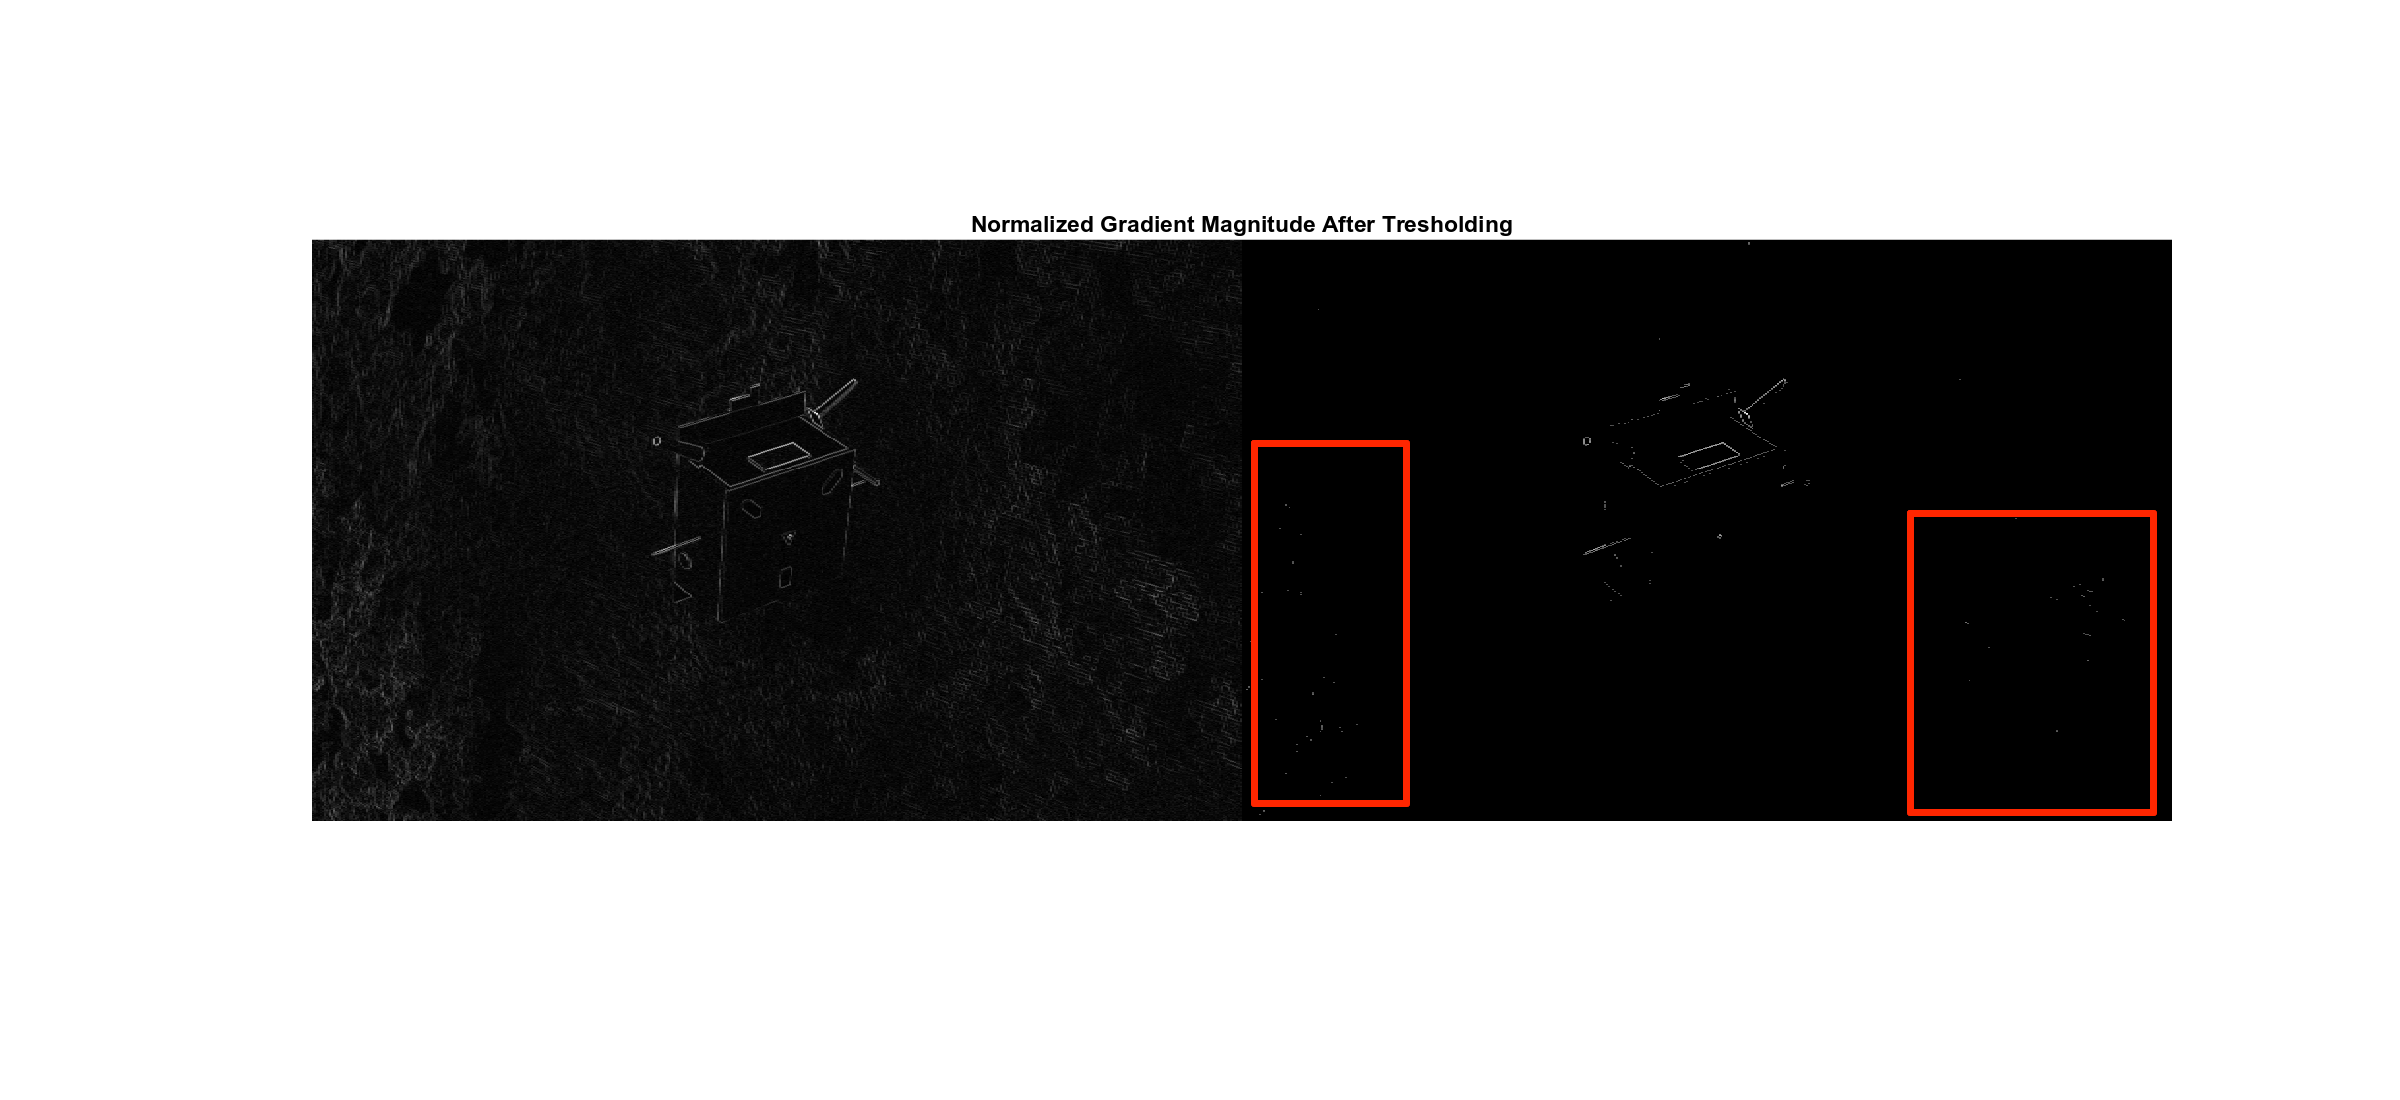
\includegraphics[width=1.0\textwidth]{gfx/results/prisma/117/8Select.png}
  \caption{Gradient image of Figure~\ref{fig:roiResults1}h. Left is normalized gradient, right is normalized gradient after tresholding. The spurious points not filtered by the \acrshort{wge} technique are enclosed in the red box.}
\end{figure}

\begin{figure}[htpb]
  \centering
  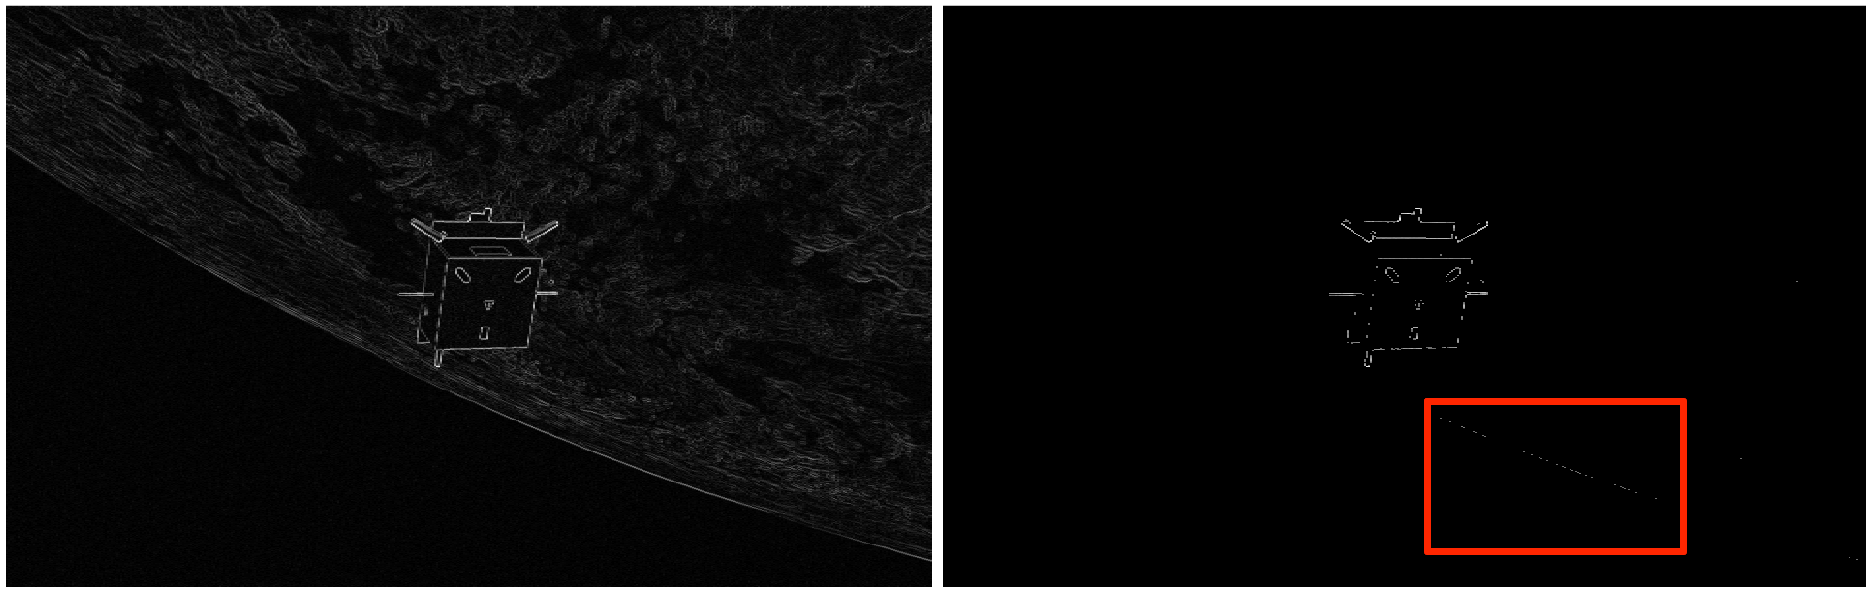
\includegraphics[width=1.0\textwidth]{gfx/results/prisma/164/8Select.png}
  \caption{Gradient image of Figure~\ref{fig:roiResults2}e. Left is normalized gradient, right is normalized gradient after tresholding. The spurious points not filtered by the \acrshort{wge} technique are enclosed in the red box.}
\end{figure}

A failure in the detection of a \acrshort{roi} involves the impossibility of rejecting spurious lines which do not belong to the silhouette of the \acrshort{sc} (as can be observed in Figures~\ref{fig:edgeDetection101}, \ref{fig:edgeDetection117} and \ref{fig:edgeDetection164}), and which would have been rejected in the case of a correct \acrshort{roi} selection. Moreover, it also affects the performances of the whole architecture, since all the quantities which are computed as multiplicative constants of the \acrshort{roi} diagonal length will be biased. On one hand, one could think to increase more the filtering depth of the image, but on the other hand this will penalize too much the analysis of images which do not have a composite background.

\begin{figure}[htpb]
  \centering
  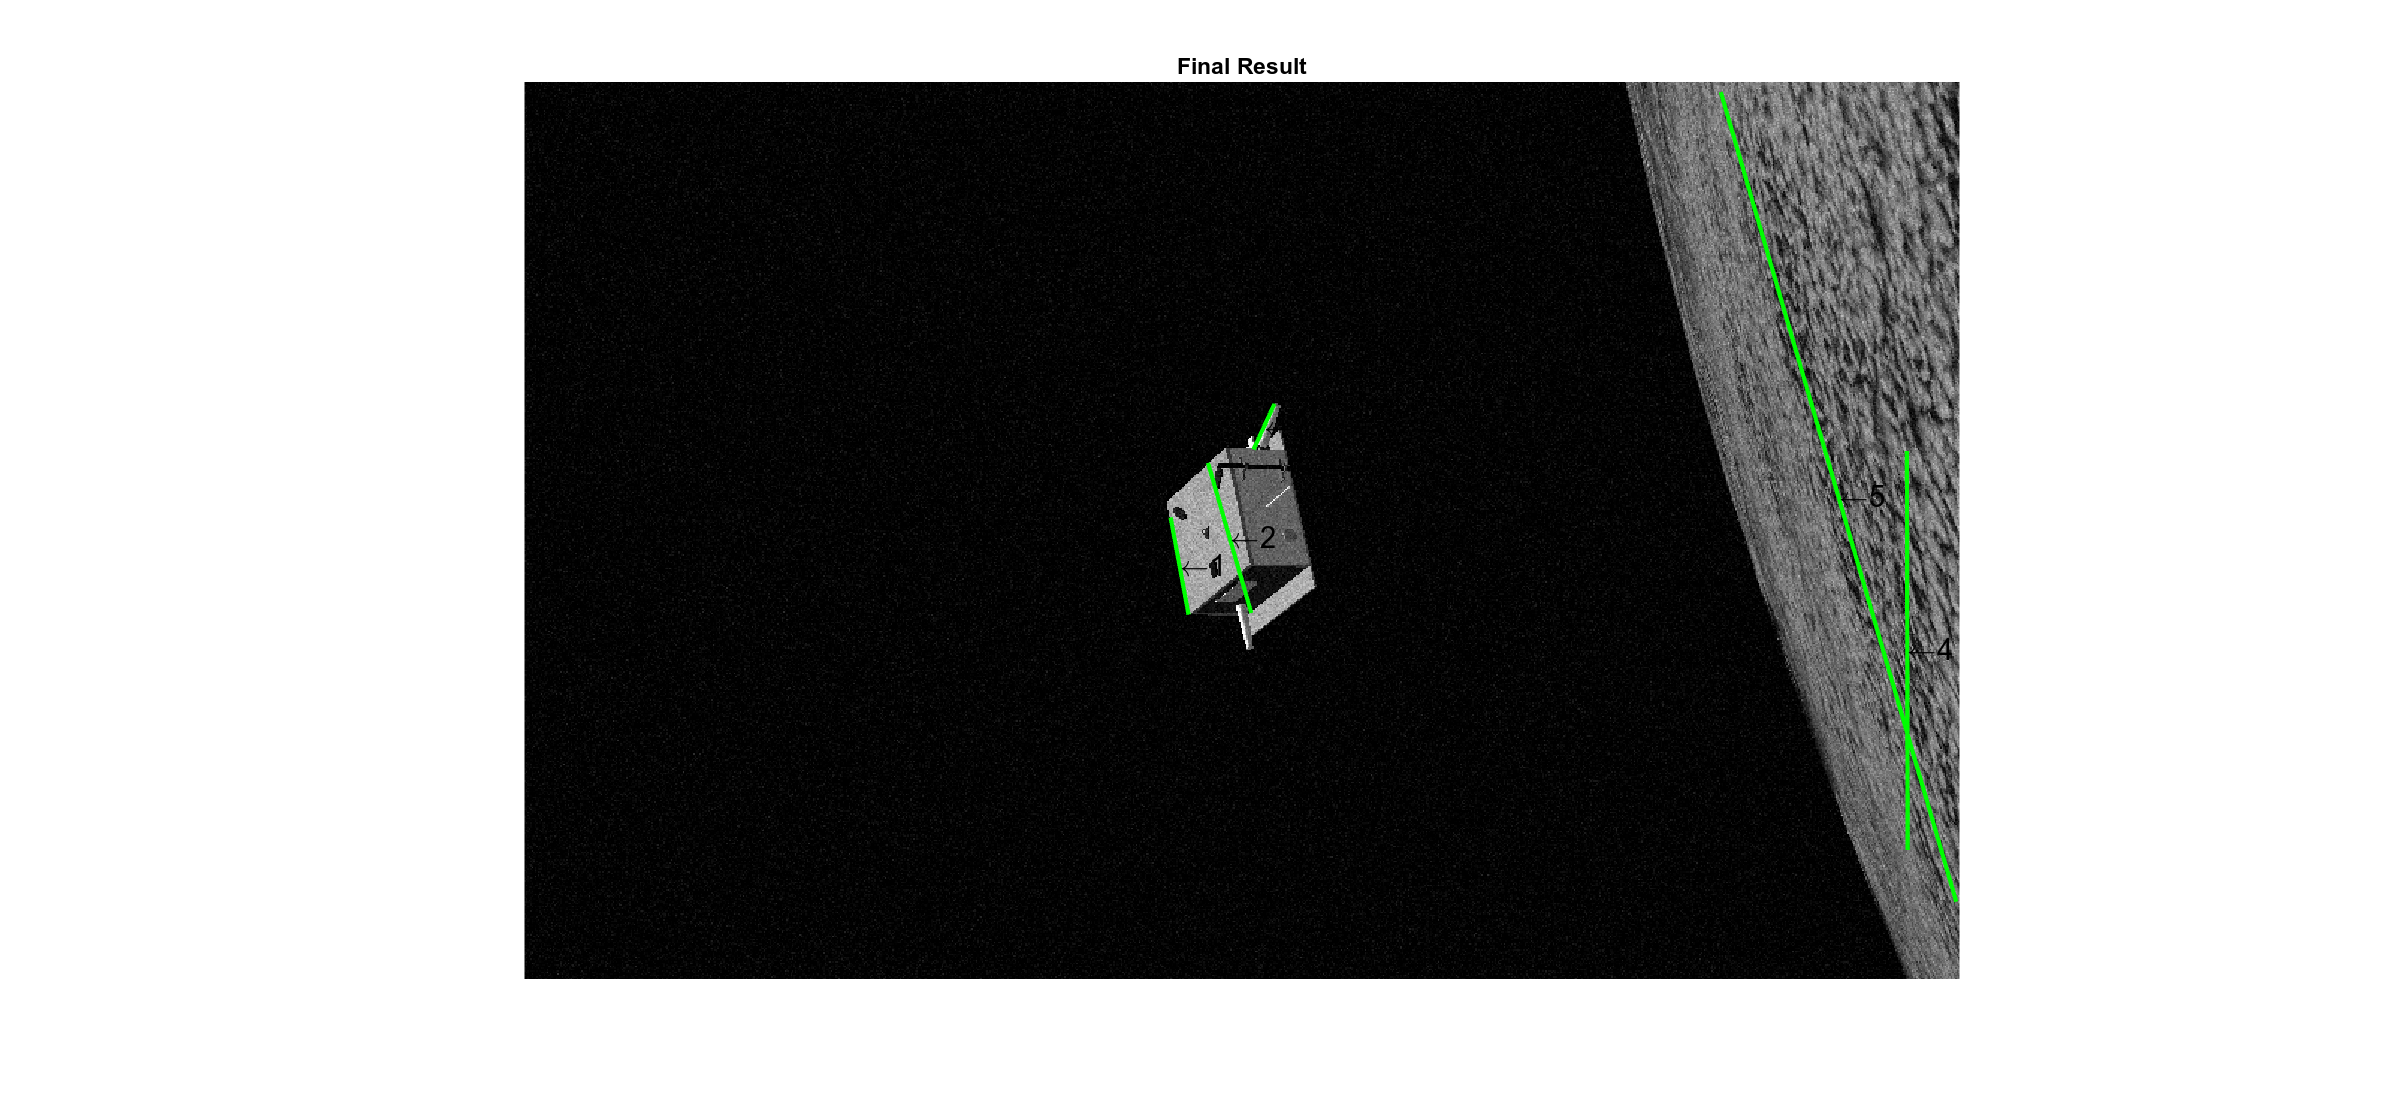
\includegraphics[width=0.82\textwidth]{gfx/results/prisma/101/15.png}
  \caption{Edge detection on Figure~\ref{fig:roiResults1}a.}
  \label{fig:edgeDetection101}
\end{figure}

\begin{figure}[htpb]
  \centering
  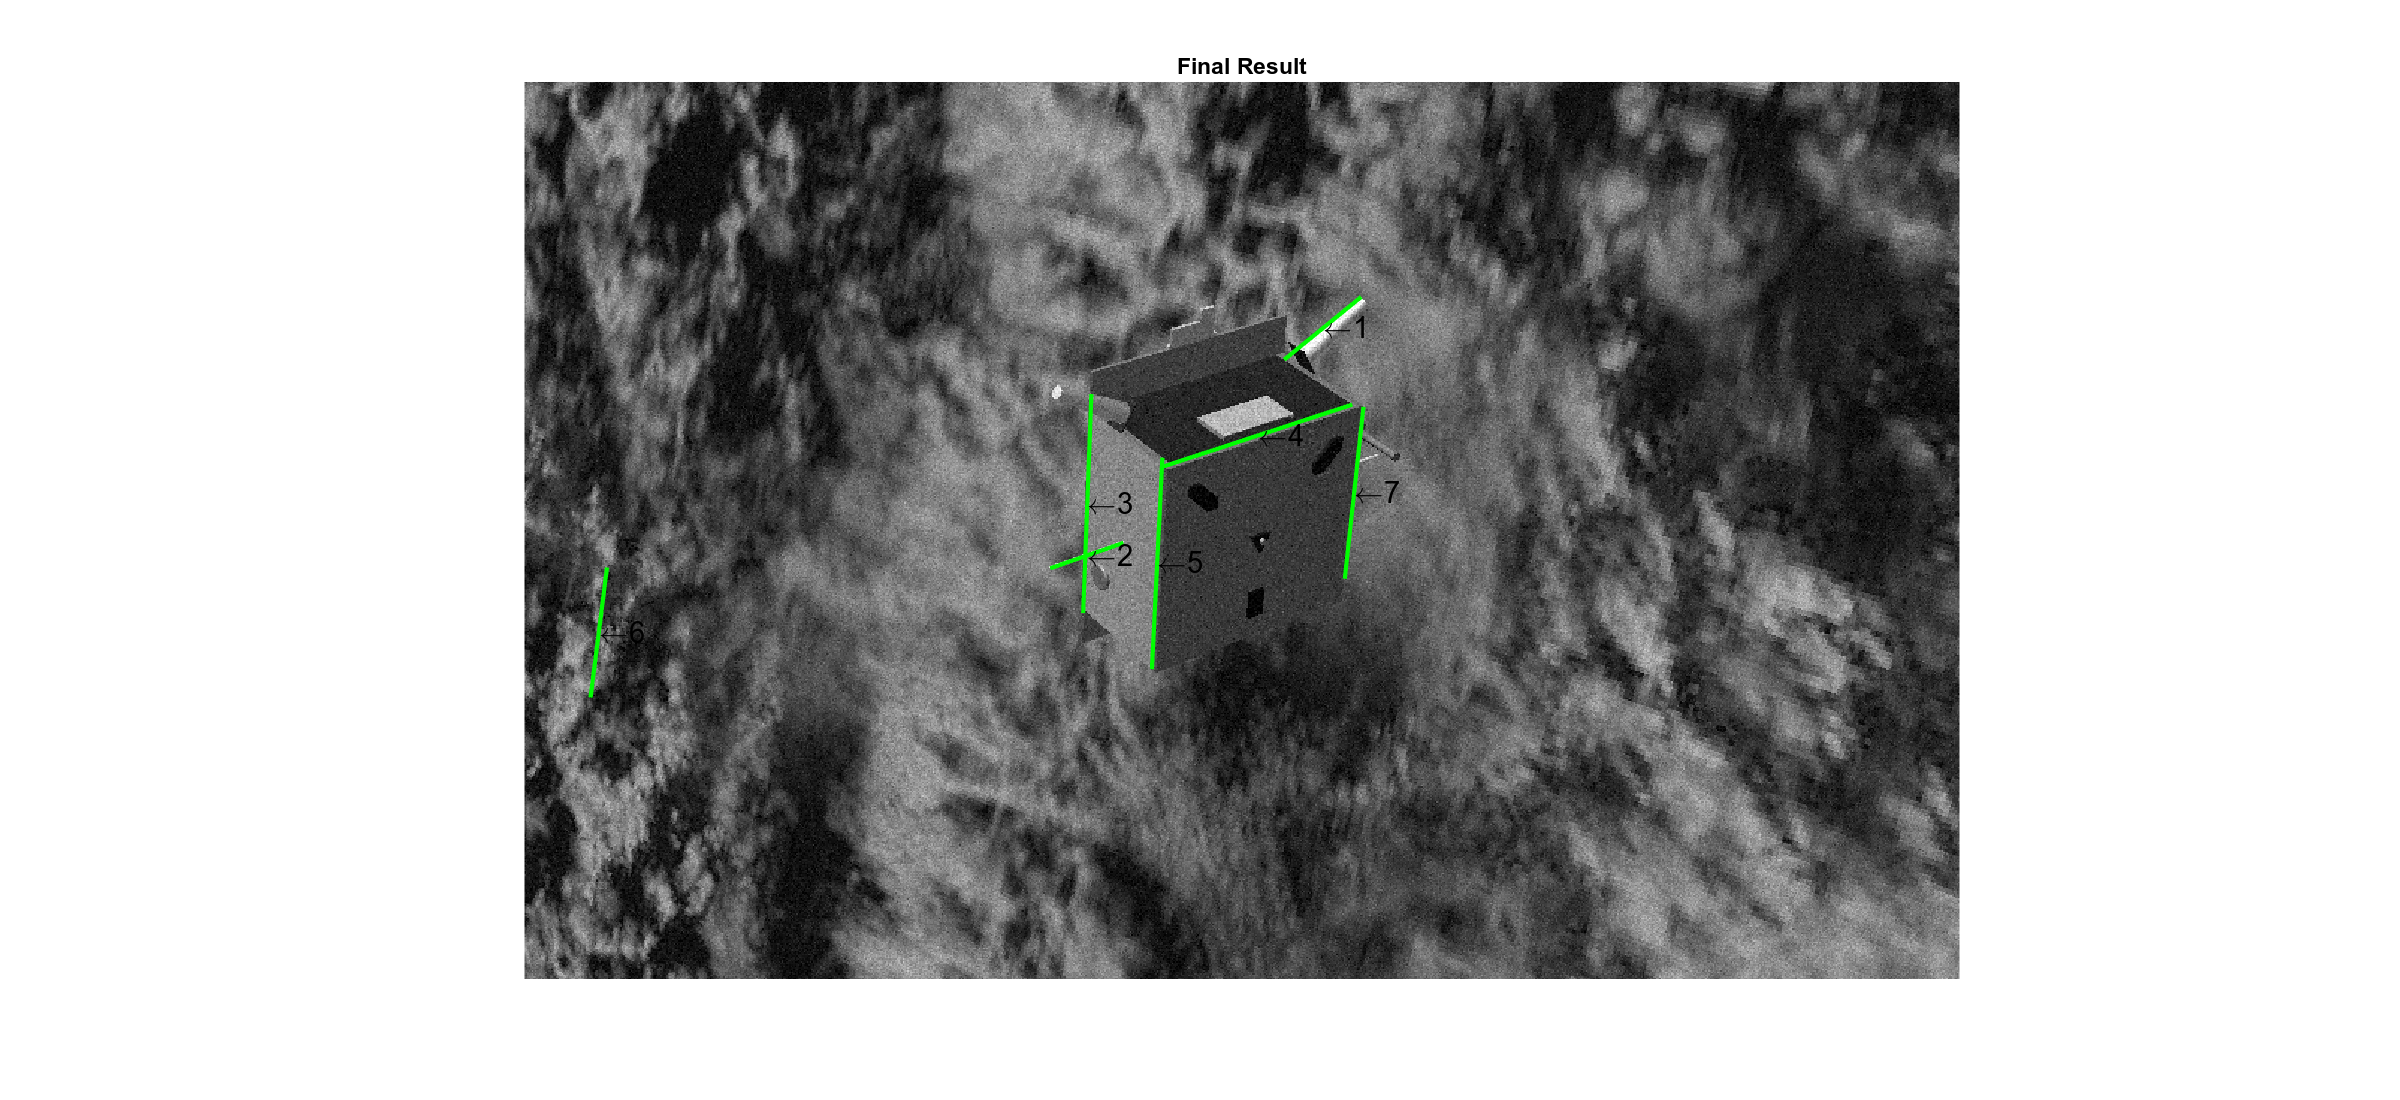
\includegraphics[width=0.82\textwidth]{gfx/results/prisma/117/15.png}
  \caption{Edge detection on Figure~\ref{fig:roiResults1}h.}
  \label{fig:edgeDetection117}
\end{figure}

\begin{figure}[htpb]
  \centering
  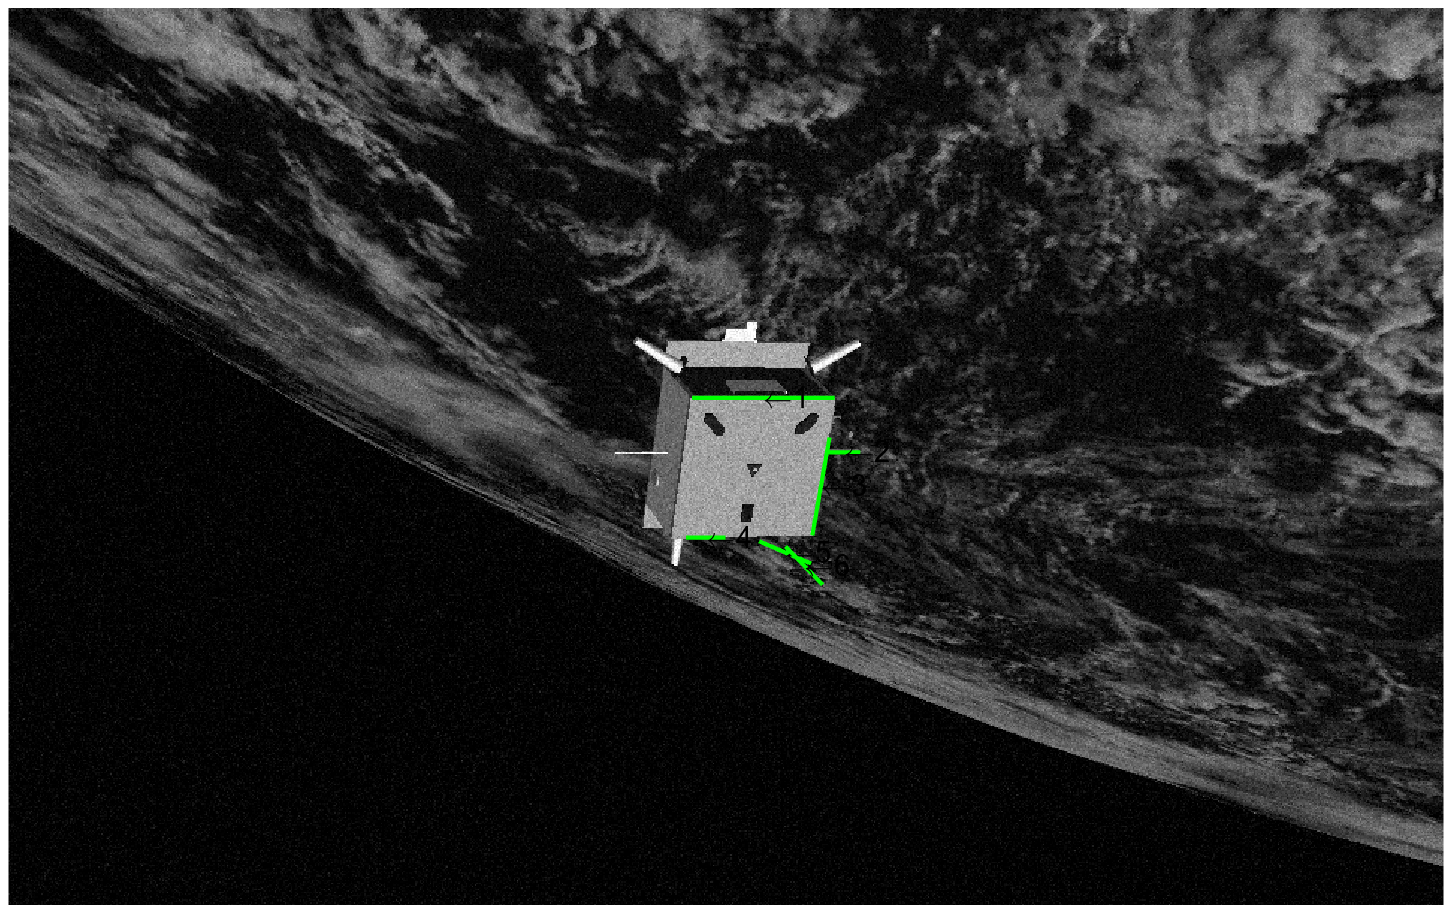
\includegraphics[width=0.82\textwidth]{gfx/results/prisma/164/15.png}
  \caption{Edge detection on Figure~\ref{fig:roiResults2}e.}
  \label{fig:edgeDetection164}
\end{figure}

For what concerns the edge detection procedure instead, as observed in \cite{Sharma2018}, further improvements must be made because it is still susceptible to producing spurious edges in some corner cases. Despite this being bad from the point of view of the \acrshort{cv} algorithm, this is good for what concerns the verification of the generated data-set, which shows the same kind of issues the SPEED data-set has. In particular, it has been observed during this work that the most critical images are the ones where the solar panels are clearly visible or when the target \acrshort{sc} is far from the camera. Regarding the former case, it is particularly evident from Figure~\ref{fig:edgeDetection204}b that the culprit is likely due to the Sobel edge detector. While all the spurious points belonging to the solar panels are filtered during by the \acrshort{wge} stream, they are not in the Sobel stream. As a result, when applying the Hough transform some spurious edges are detected which are not rejected since they fall inside the \acrshort{roi}. During the work on this thesis, some efforts have been made to cope with this issue which however has not been completely resolved, from what can bee seen in Figure~\ref{fig:edgeDetection204}c. On one hand, more tresholds could be introduced into the image processing subsystem to take into account the presence of short spurious line and and remove them. On the other hand however, is really hard to fine tune those tresholds in order to not remove other short edges which instead are useful, such as antennas.

\begin{figure}[htpb]
  \centering
  \subfloat[\acrshort{wge} stream output.]{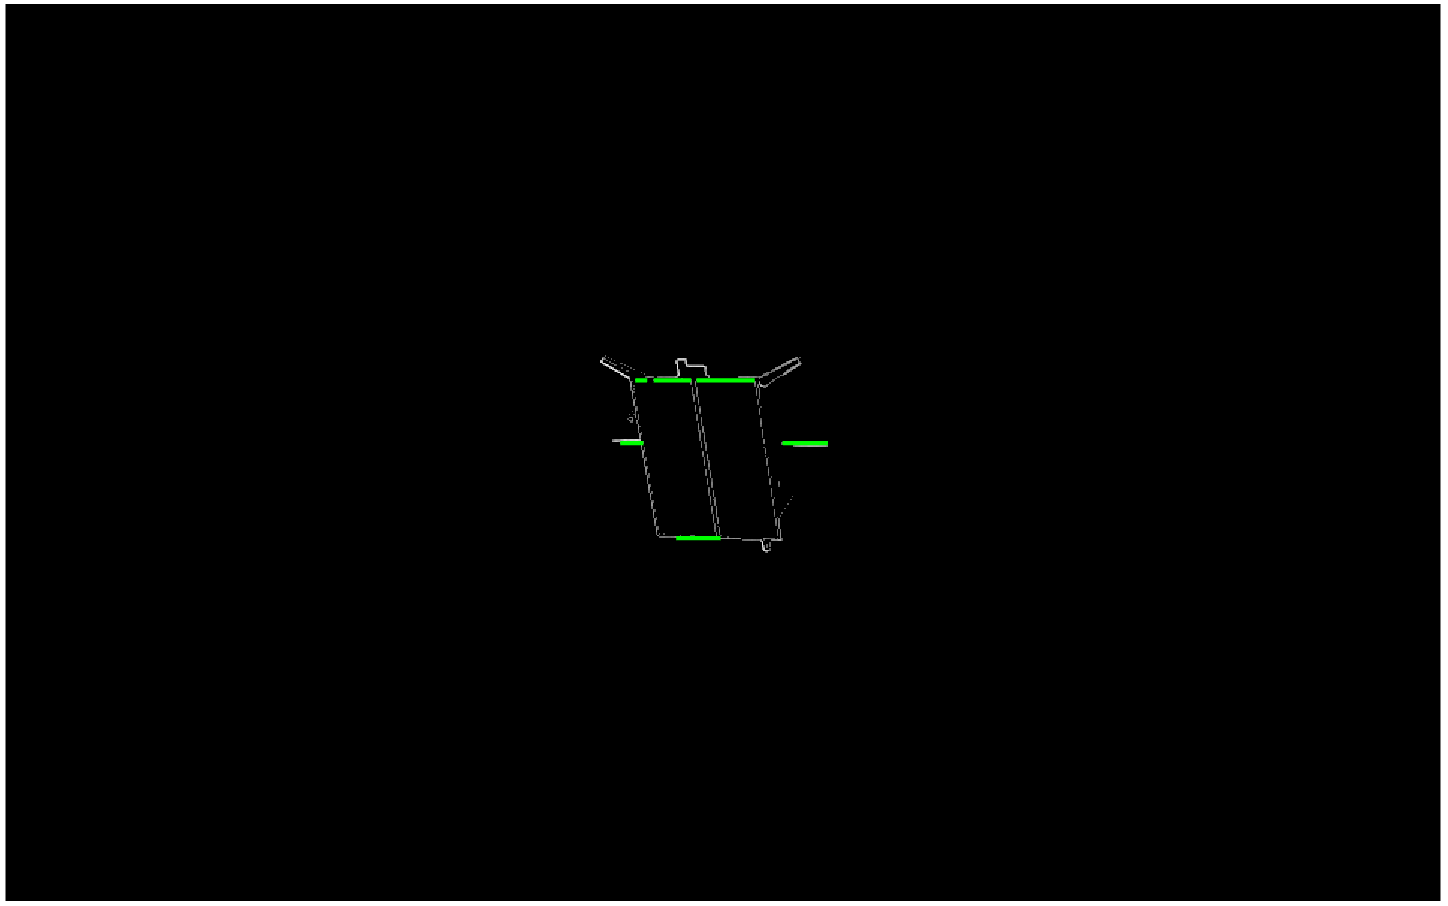
\includegraphics[width=0.47\textwidth]{gfx/results/prisma/204/10.png}}
  \qquad
  \subfloat[\acrshort{seh} stream output.]{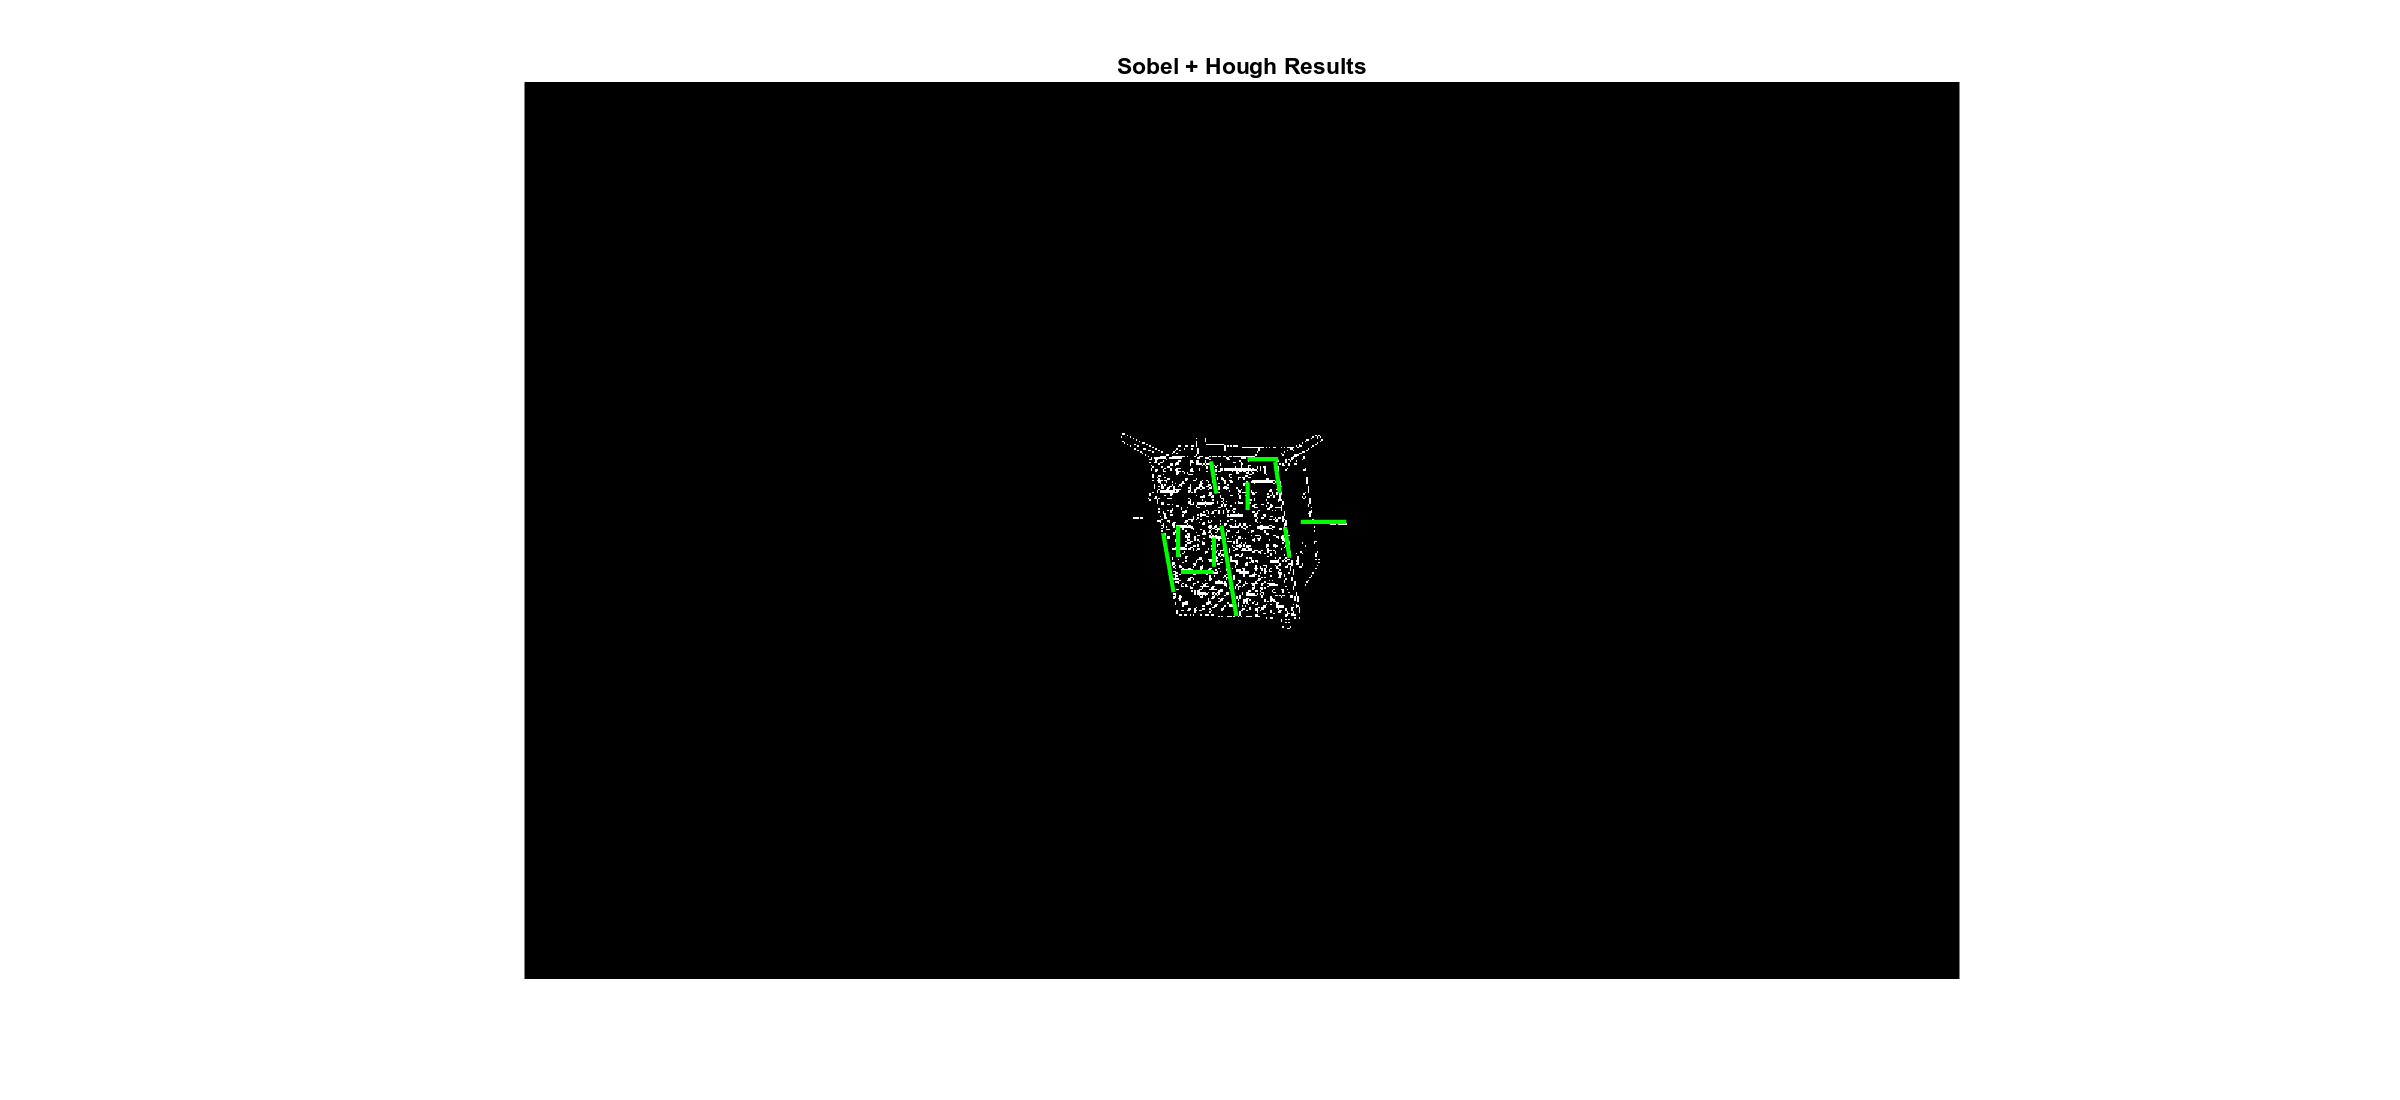
\includegraphics[width=0.47\textwidth]{gfx/results/prisma/204/11.png}}
  \qquad
  \subfloat[\acrshort{wge} and \acrshort{seh} streams after the merge stream procedure.]{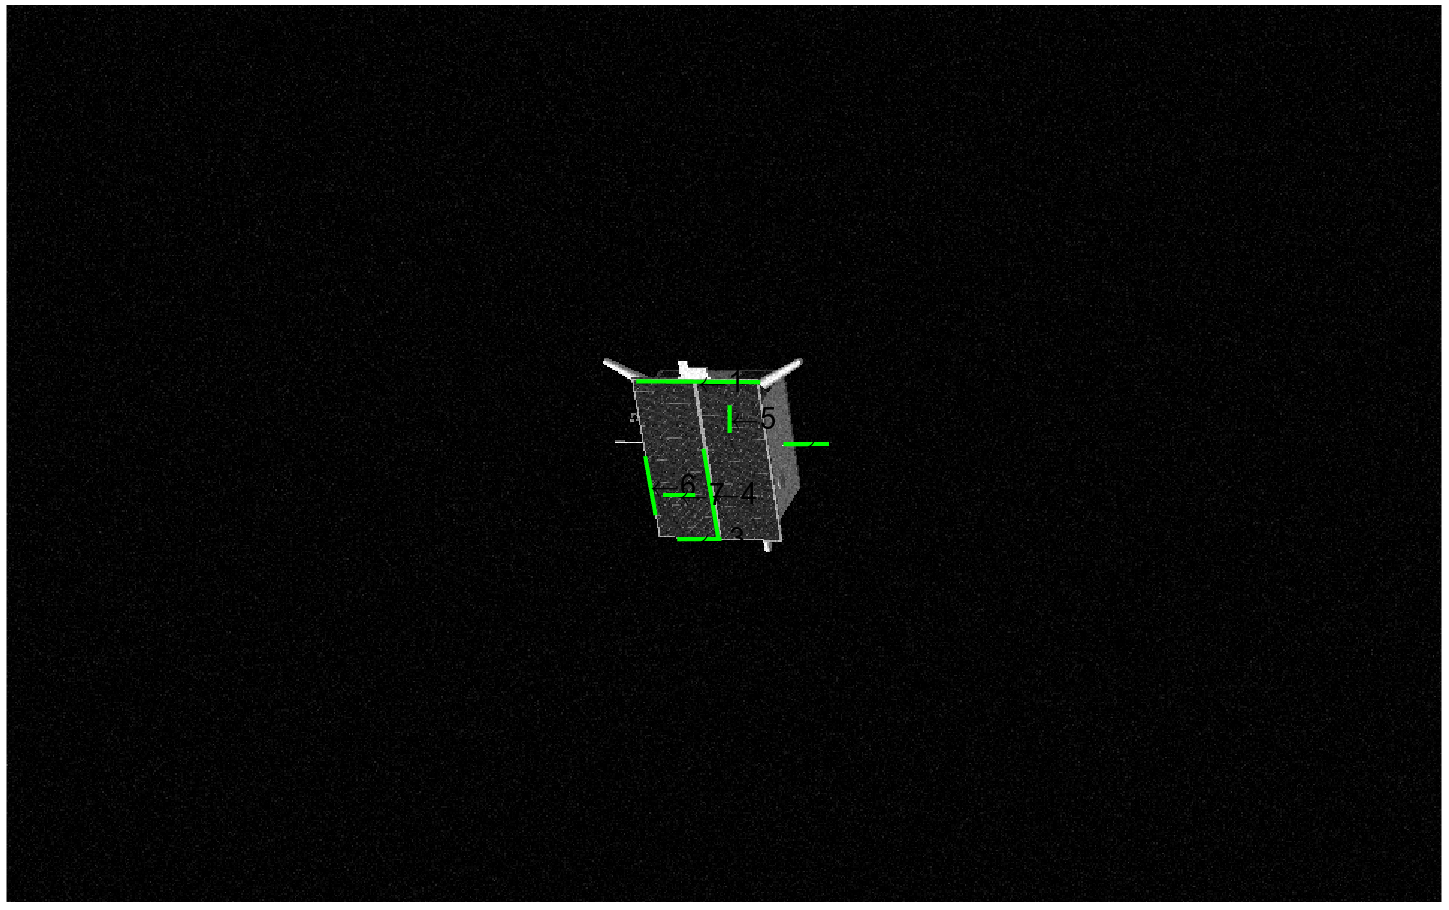
\includegraphics[width=0.47\textwidth]{gfx/results/prisma/204/15.png}}
  \qquad
  \caption{Image where the image processing subsystem contained spurious edges due to the presence of the solar panels.}
  \label{fig:edgeDetection204}
\end{figure}

There are also some particular attitudes where the Hough transform fails on the \acrshort{wge} filtered image, if the inter-spacecraft distance is relatively far. Taking as an example what's shown in Figure~\ref{fig:edgeDetection82} this can be likely due to the fact that the initial blur done to in order to filter out noise makes edges of the \acrshort{sc} harder to distinguish for the Hough transform. So, in general, the algorithm will loose accuracy as the relative distance grows.

\begin{figure}[htpb]
  \centering
  \subfloat[Normalized gradient after tresholding.]{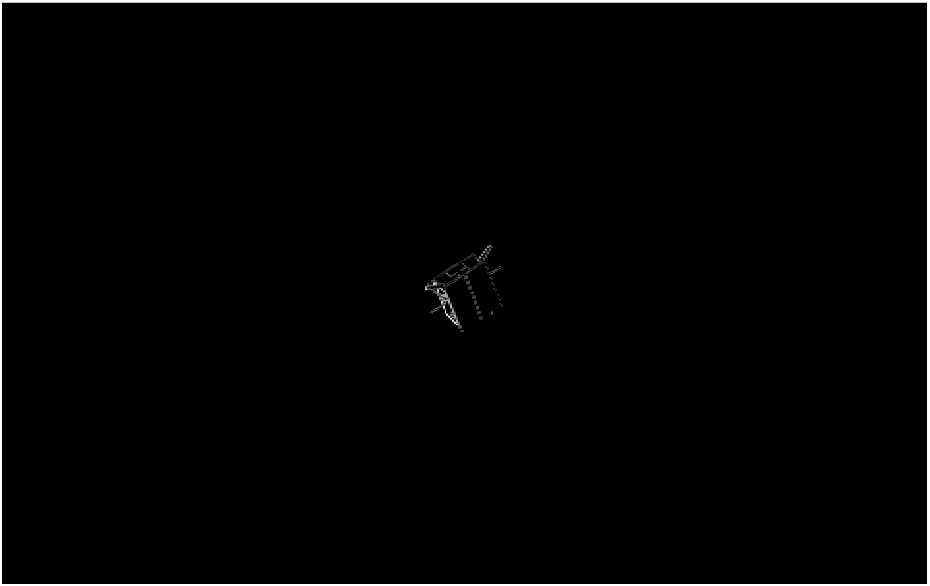
\includegraphics[width=0.47\textwidth]{gfx/results/prisma/82/8aftertresholding.png}}
  \qquad
  \subfloat[\acrshort{wge} and Hough result.]{\includegraphics[width=0.47\textwidth]{gfx/results/prisma/82/10.png}}
  \qquad
  \subfloat[\acrshort{seh} result.]{\includegraphics[width=0.47\textwidth]{gfx/results/prisma/82/11.png}}
  \qquad
  \subfloat[Final result.]{\includegraphics[width=0.47\textwidth]{gfx/results/prisma/82/15.png}}
  \qquad
  \caption{Image where the image processing subsystem contained not correctly detected edges.}
  \label{fig:edgeDetection82}
\end{figure}

In Figures~\ref{fig:translationalErrorHist} and \ref{fig:rotationalErrorHist} are showed the histograms of the translational an the rotational errors computed over a set of 50 images. The mean values obtained are \SI{0.2506}{\m} for the translational error and $0.0528^\circ$ for the rotational error respectively.

\begin{figure}[htpb]
  \centering
  \includegraphics[width=0.9\textwidth]{gfx/plotError/transHist.eps}
  \caption{Translational Error (histogram).}
  \label{fig:translationalErrorHist}
\end{figure}

\begin{figure}[htpb]
  \centering
  \includegraphics[width=0.9\textwidth]{gfx/plotError/rotHist.eps}
  \caption{Rotational Error (histogram).}
  \label{fig:rotationalErrorHist}
\end{figure}

Figures~\ref{fig:transAndDist} and \ref{fig:rotAndDist} instead shows the variation of the translational and rotational error as the inter-spacecraft distance increases. While for the translational error there is an increasing trend as the relative distance grows, there isn't any evince of a trend for what concerns the rotational error.

\begin{figure}[htpb]
  \centering
  \includegraphics[width=0.9\textwidth]{gfx/plotError/transAndDist.eps}
  \caption{Translational error related to inter-spacecraft distance.}
  \label{fig:transAndDist}
\end{figure}

\begin{figure}[htpb]
  \centering
  \includegraphics[width=0.9\textwidth]{gfx/plotError/rotAndDist.eps}
  \caption{Rotational error related to inter-spacecraft distance.}
  \label{fig:rotAndDist}
\end{figure}

Lastly, Figure~\ref{fig:c3c2c1} shows the variation of the error with respect to camera axis. As it can be seen, there is no evidence of a privileged axis which behaves better or worse with respect to the others.

\begin{figure}[htpb]
  \centering
  \includegraphics[width=0.9\textwidth]{gfx/plotError/c3c2c1.eps}
  \caption{Error with respect to camera axis.}
  \label{fig:c3c2c1}
\end{figure}
